% Side-by-side comparison with Improved Mean Flow (iMF)
% Showing ALL overlapping ImageNet classes (sorted by class number)

\begin{figure*}[p]
    \centering
    % Header
    \begin{minipage}{0.48\textwidth}
        \centering{ours}
    \end{minipage}\hfill
    \begin{minipage}{0.48\textwidth}
        \centering{improved MeanFlow (iMF)}
    \end{minipage}\\[0.2em]
    
    % Class 012: House finch
    \begin{minipage}[b]{0.48\textwidth}
        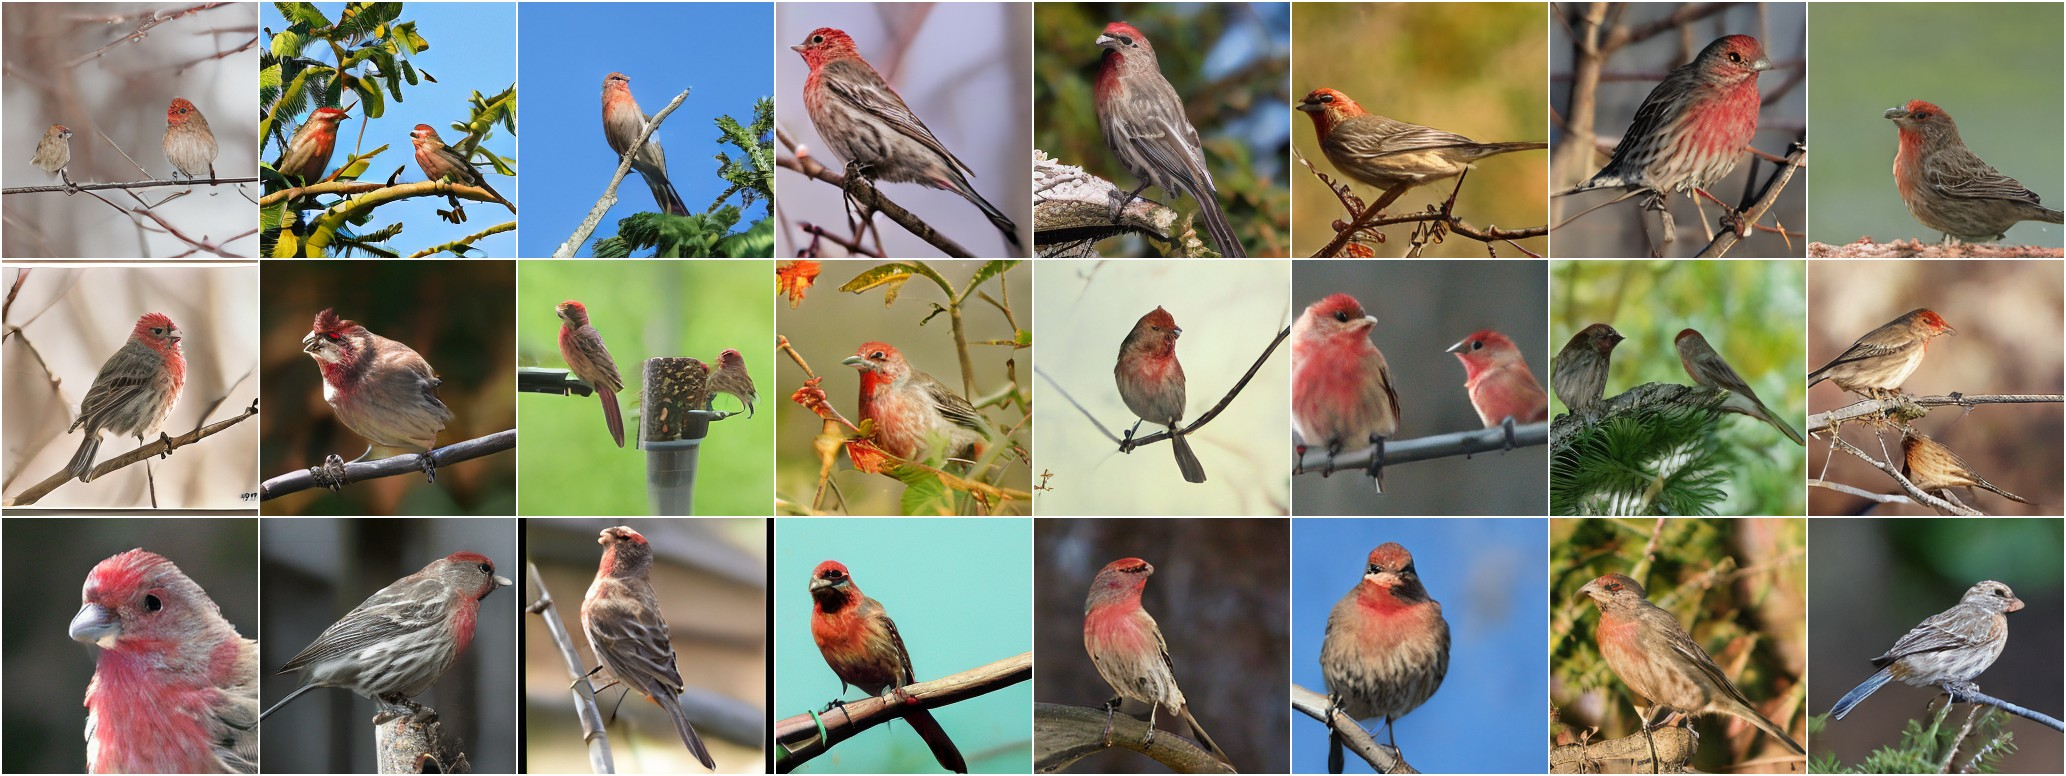
\includegraphics[width=\linewidth]{figures/imf_images/drift/classrank0086_class012_house_finch_score5.09.jpg}
    \end{minipage}\hfill
    \begin{minipage}[b]{0.48\textwidth}
        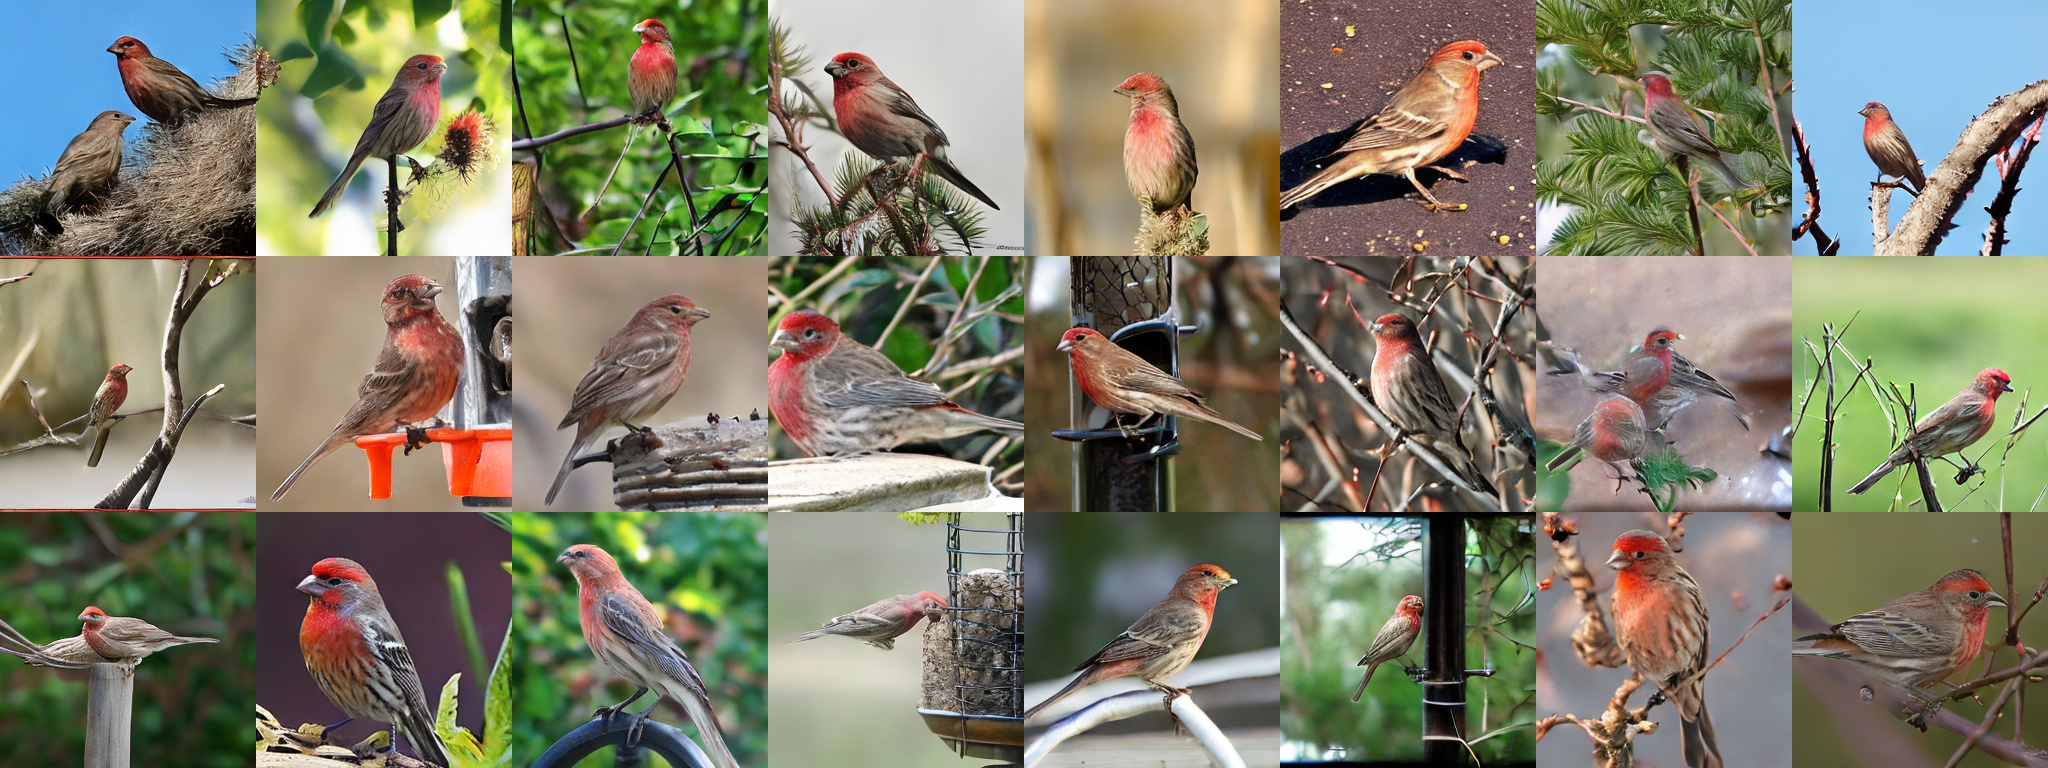
\includegraphics[width=\linewidth]{figures/imf_images/12.jpg}
    \end{minipage}\\[-0.2em]
    \centering\small Class 012: House finch\\[0.2em]
    
    % Class 014: Indigo bunting
    \begin{minipage}[b]{0.48\textwidth}
        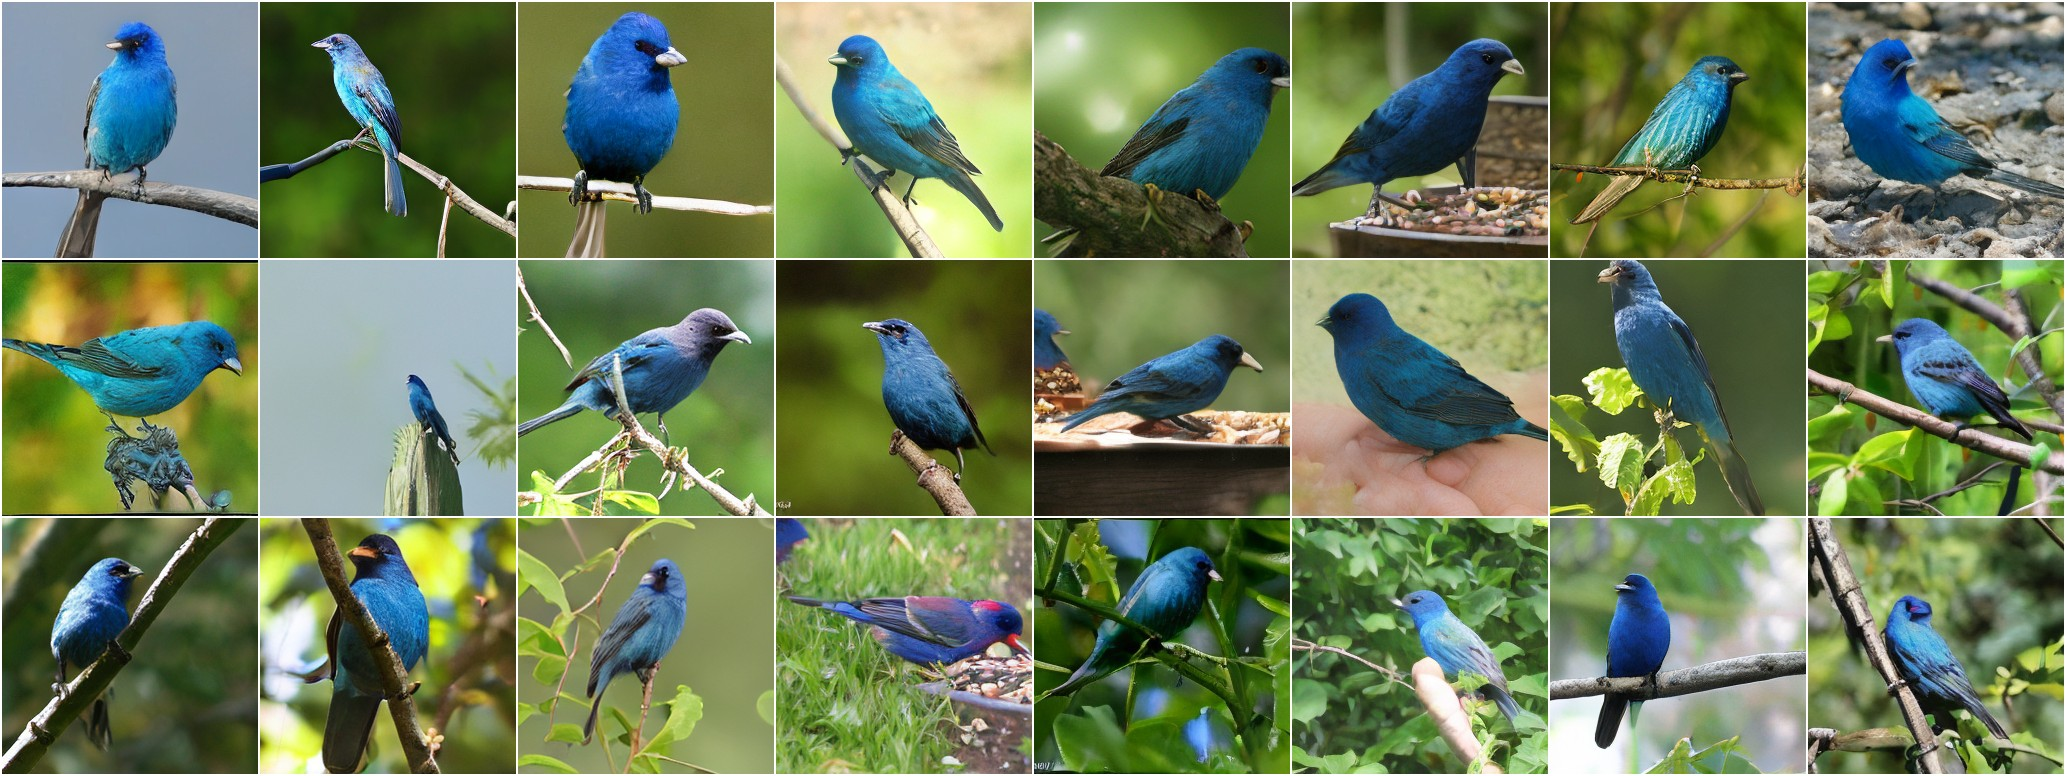
\includegraphics[width=\linewidth]{figures/imf_images/drift/classrank0071_class014_indigo_bunting_score5.12.jpg}
    \end{minipage}\hfill
    \begin{minipage}[b]{0.48\textwidth}
        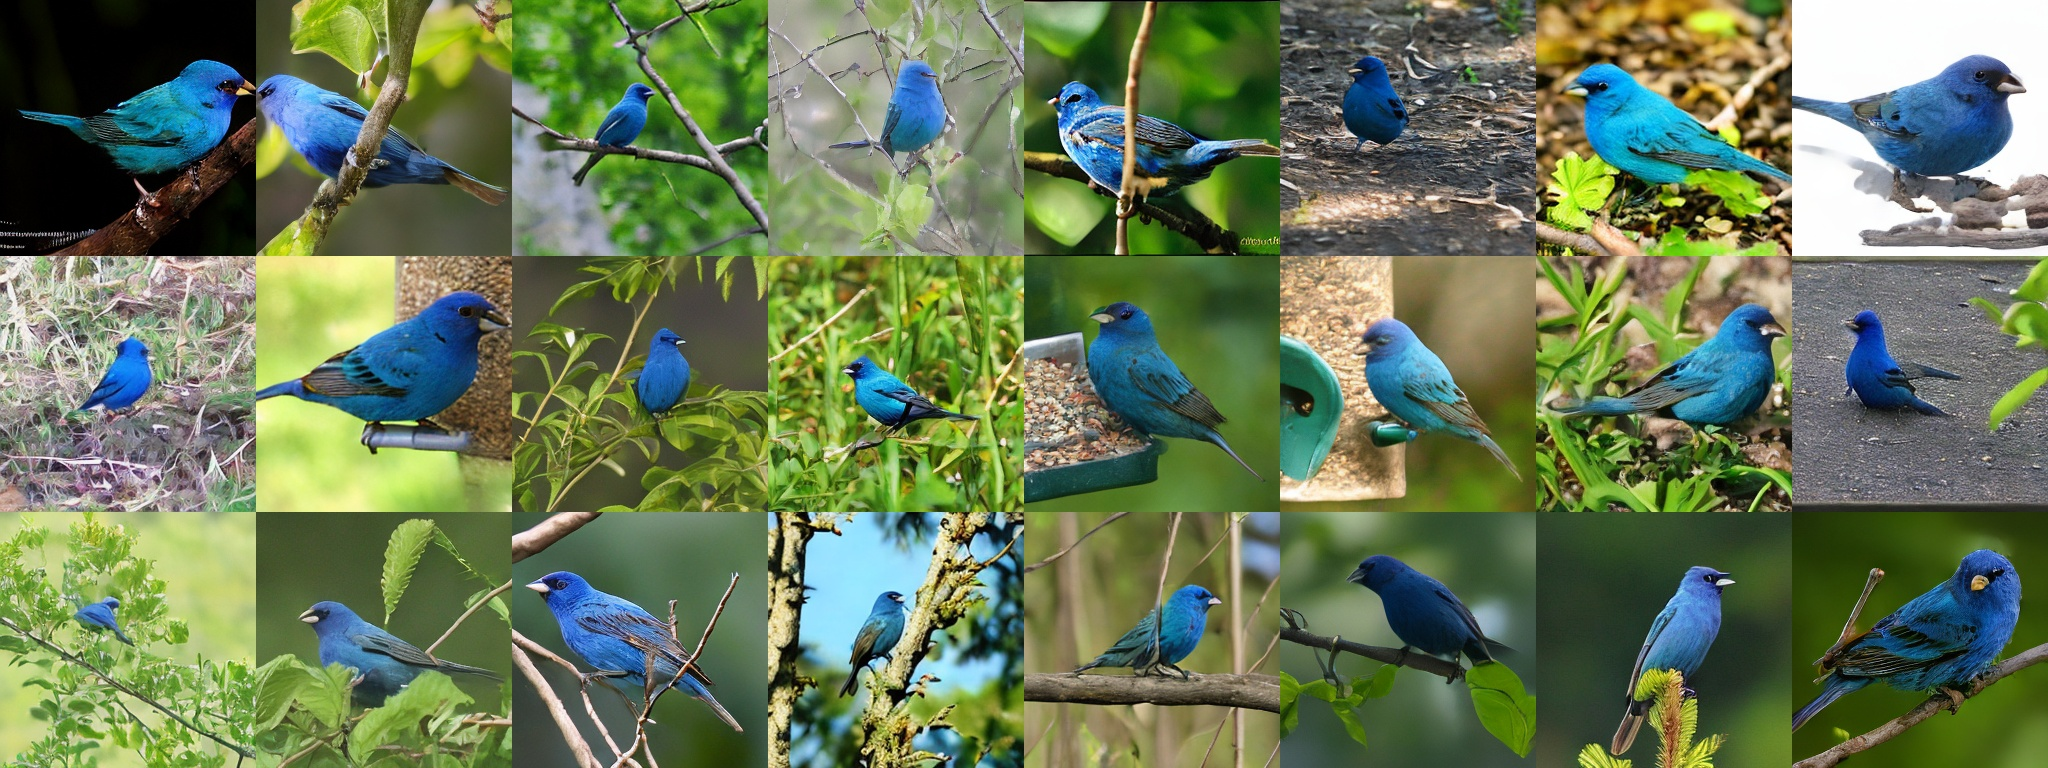
\includegraphics[width=\linewidth]{figures/imf_images/14.jpg}
    \end{minipage}\\[-0.2em]
    \centering\small Class 014: Indigo bunting\\[0.2em]
    
    % Class 022: Bald eagle
    \begin{minipage}[b]{0.48\textwidth}
        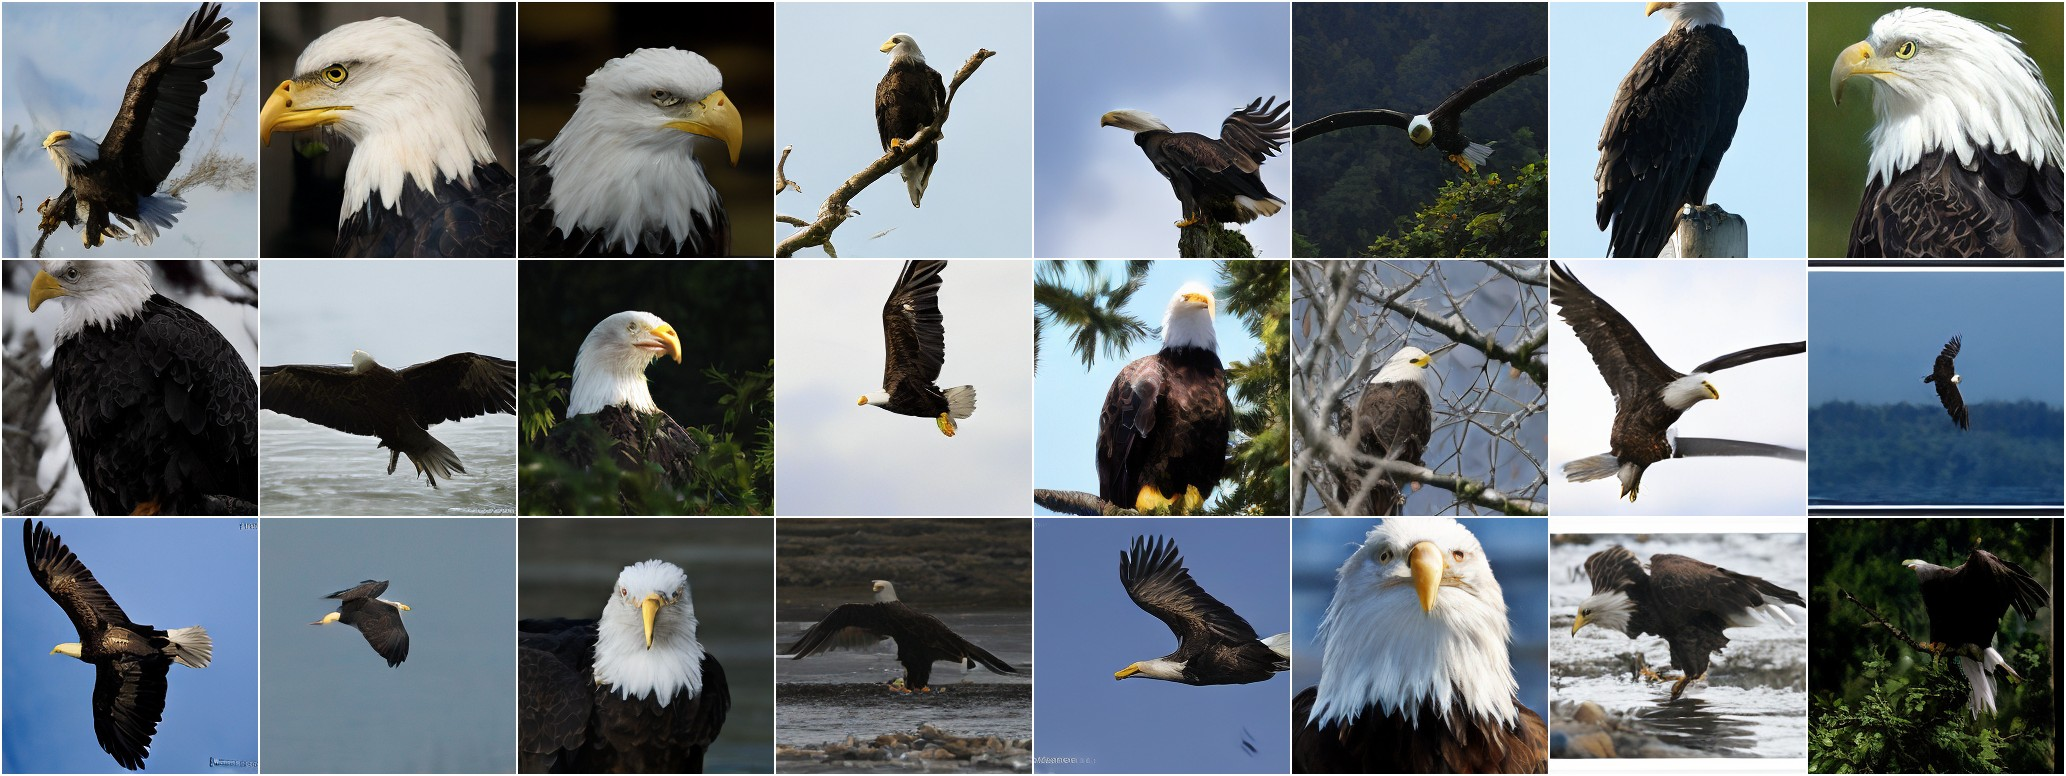
\includegraphics[width=\linewidth]{figures/imf_images/drift/classrank0039_class022_bald_eagle_score5.21.jpg}
    \end{minipage}\hfill
    \begin{minipage}[b]{0.48\textwidth}
        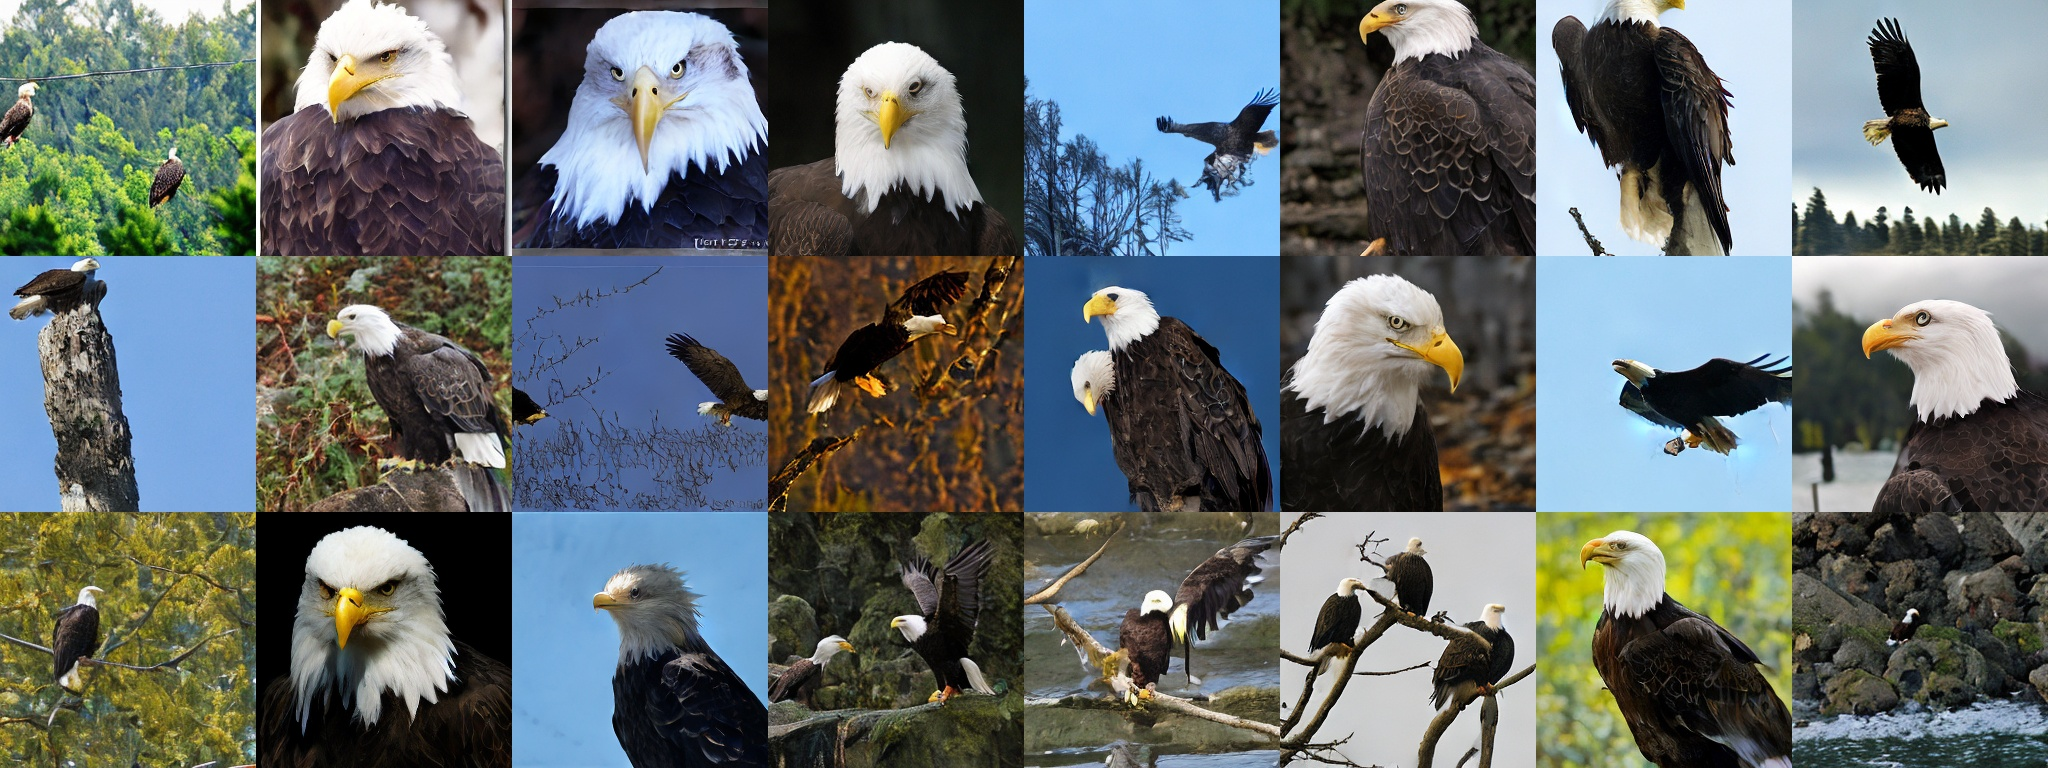
\includegraphics[width=\linewidth]{figures/imf_images/22.jpg}
    \end{minipage}\\[-0.2em]
    \centering\small Class 022: Bald eagle\\[0.2em]
    
    % Class 042: Agama
    \begin{minipage}[b]{0.48\textwidth}
        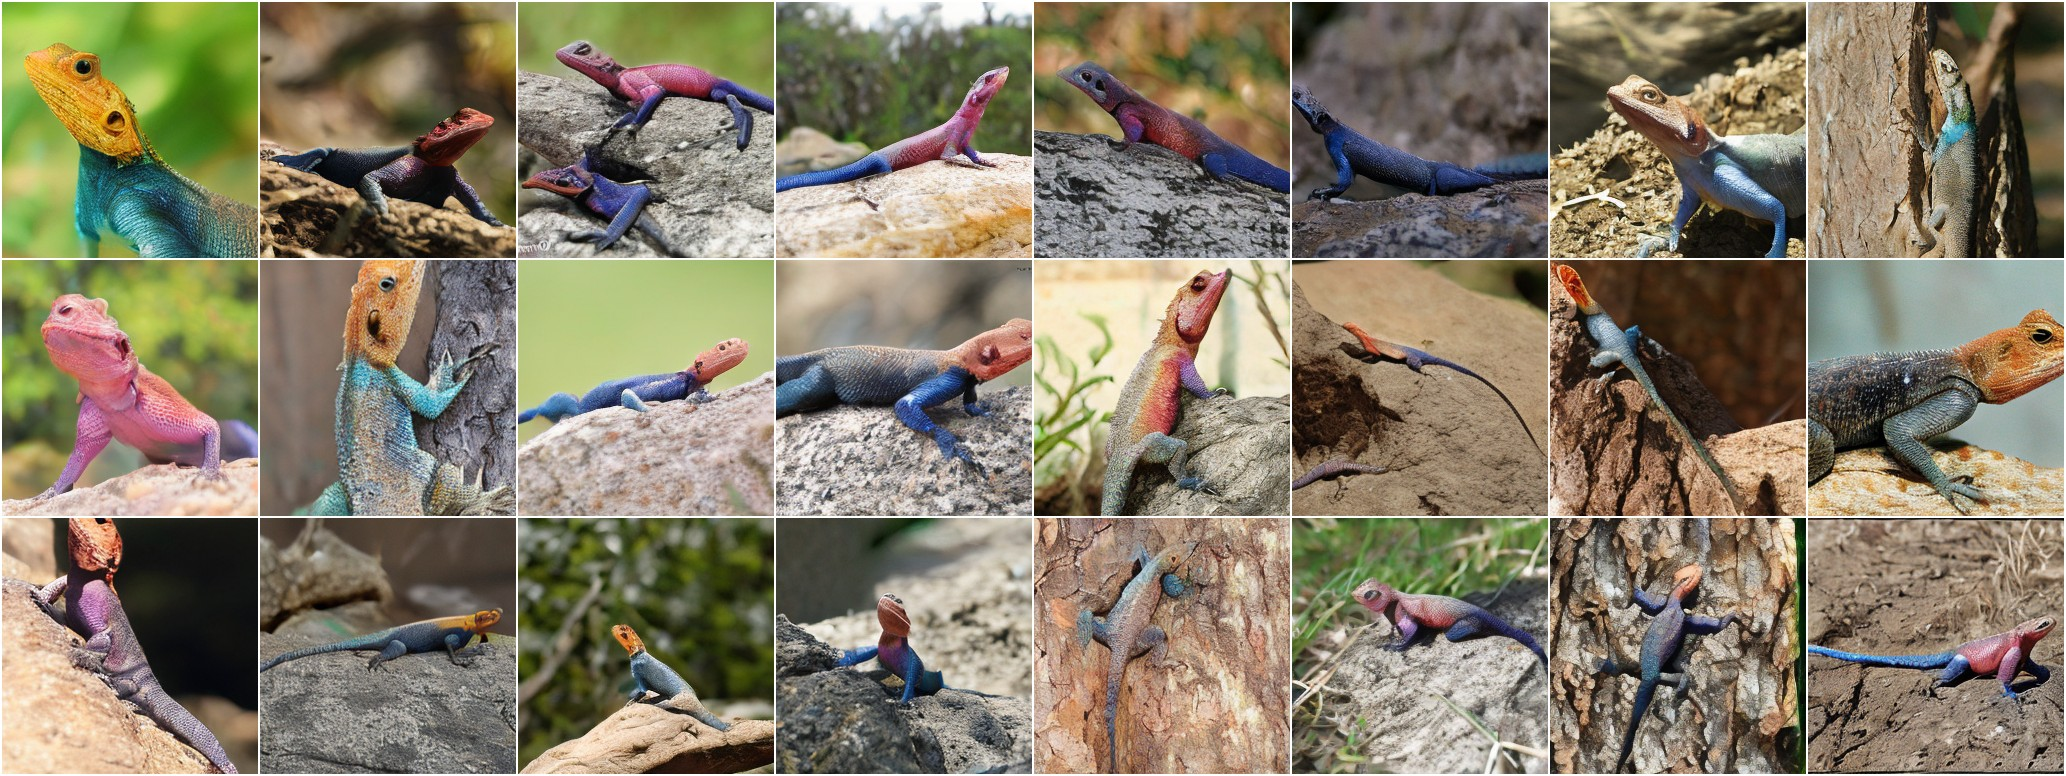
\includegraphics[width=\linewidth]{figures/imf_images/drift/classrank0107_class042_agama_score5.06.jpg}
    \end{minipage}\hfill
    \begin{minipage}[b]{0.48\textwidth}
        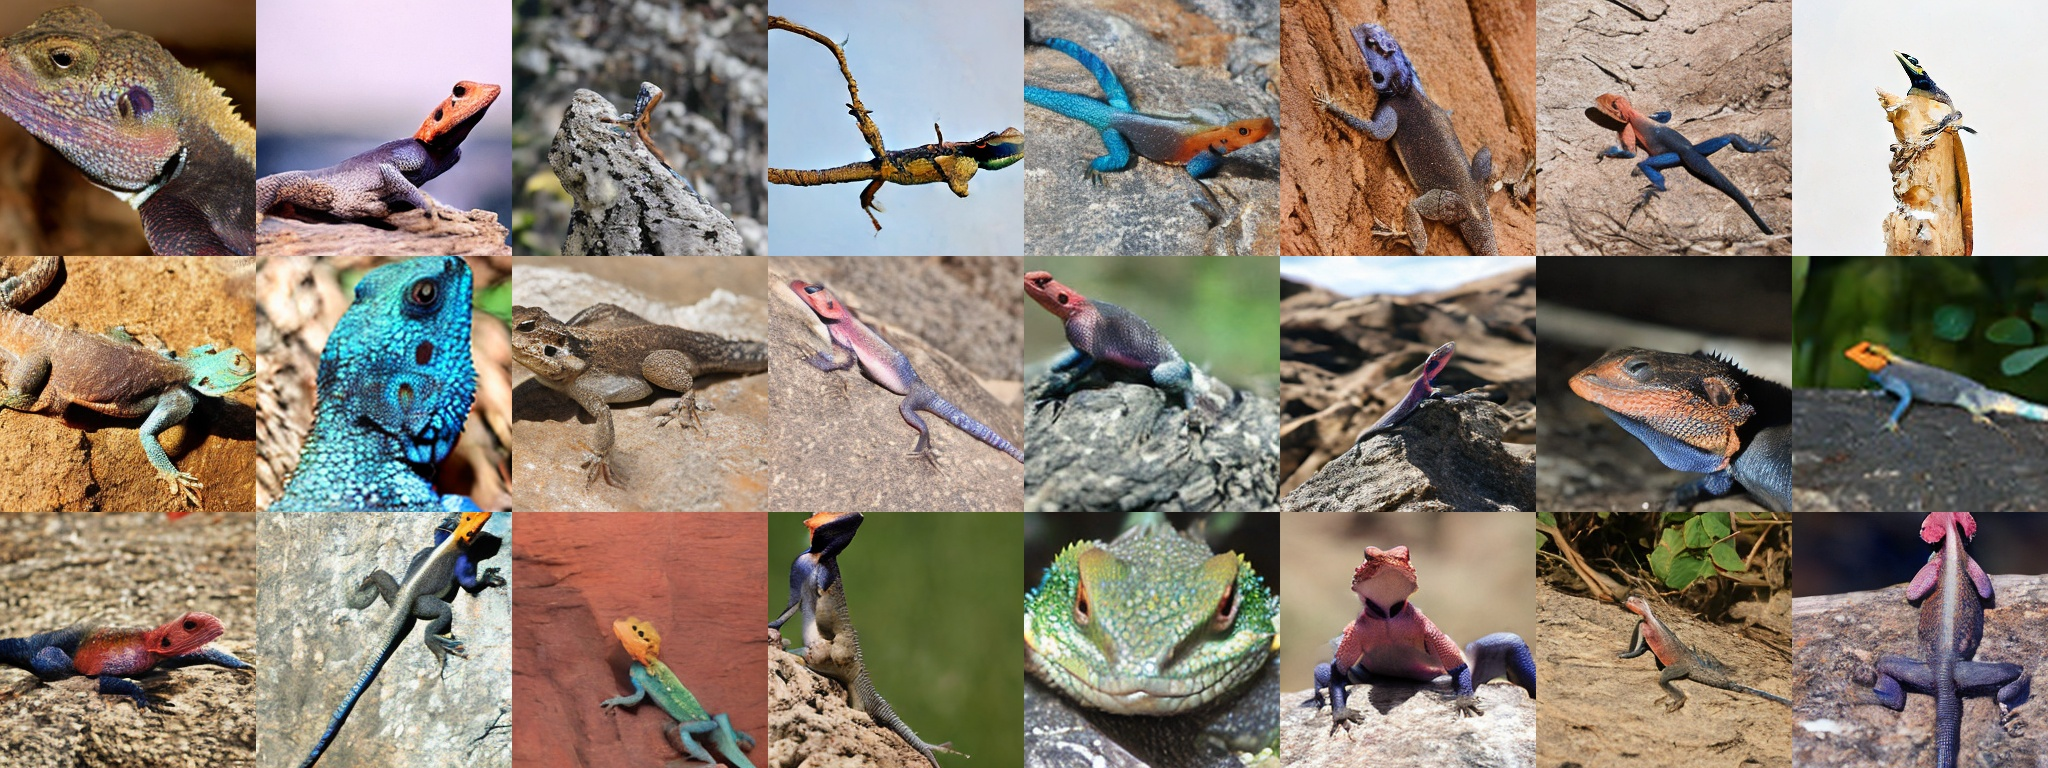
\includegraphics[width=\linewidth]{figures/imf_images/42.jpg}
    \end{minipage}\\[-0.2em]
    \centering\small Class 042: Agama\\[0.2em]
    
    % Class 081: Ptarmigan
    \begin{minipage}[b]{0.48\textwidth}
        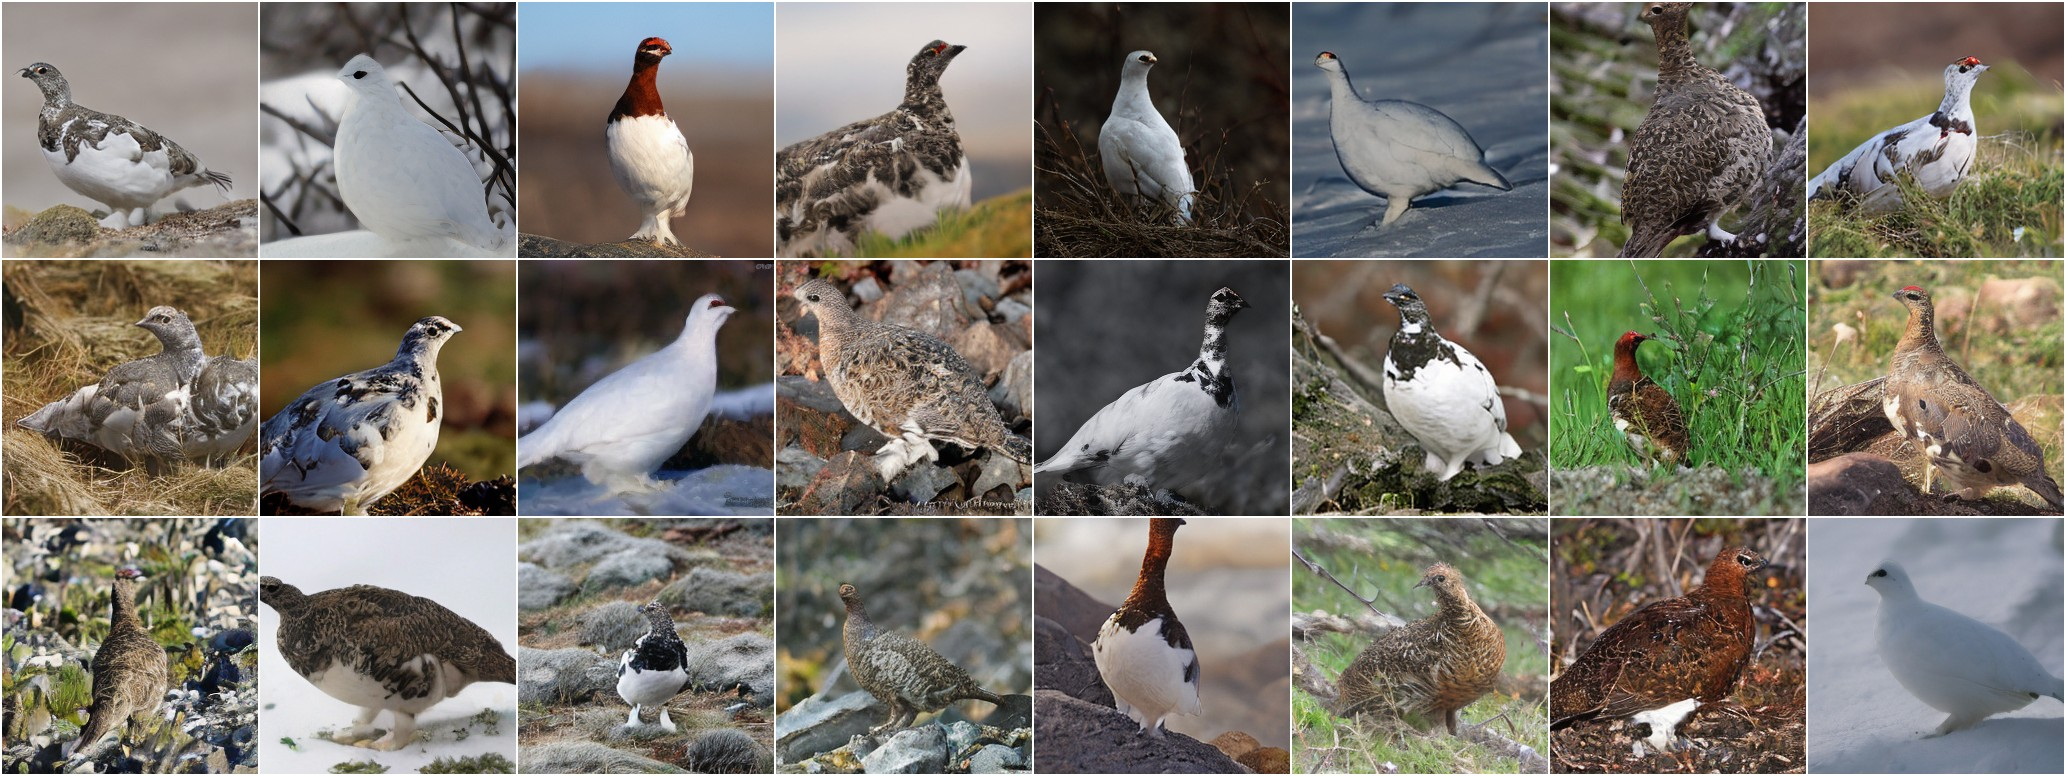
\includegraphics[width=\linewidth]{figures/imf_images/drift/classrank0333_class081_ptarmigan_score4.78.jpg}
    \end{minipage}\hfill
    \begin{minipage}[b]{0.48\textwidth}
        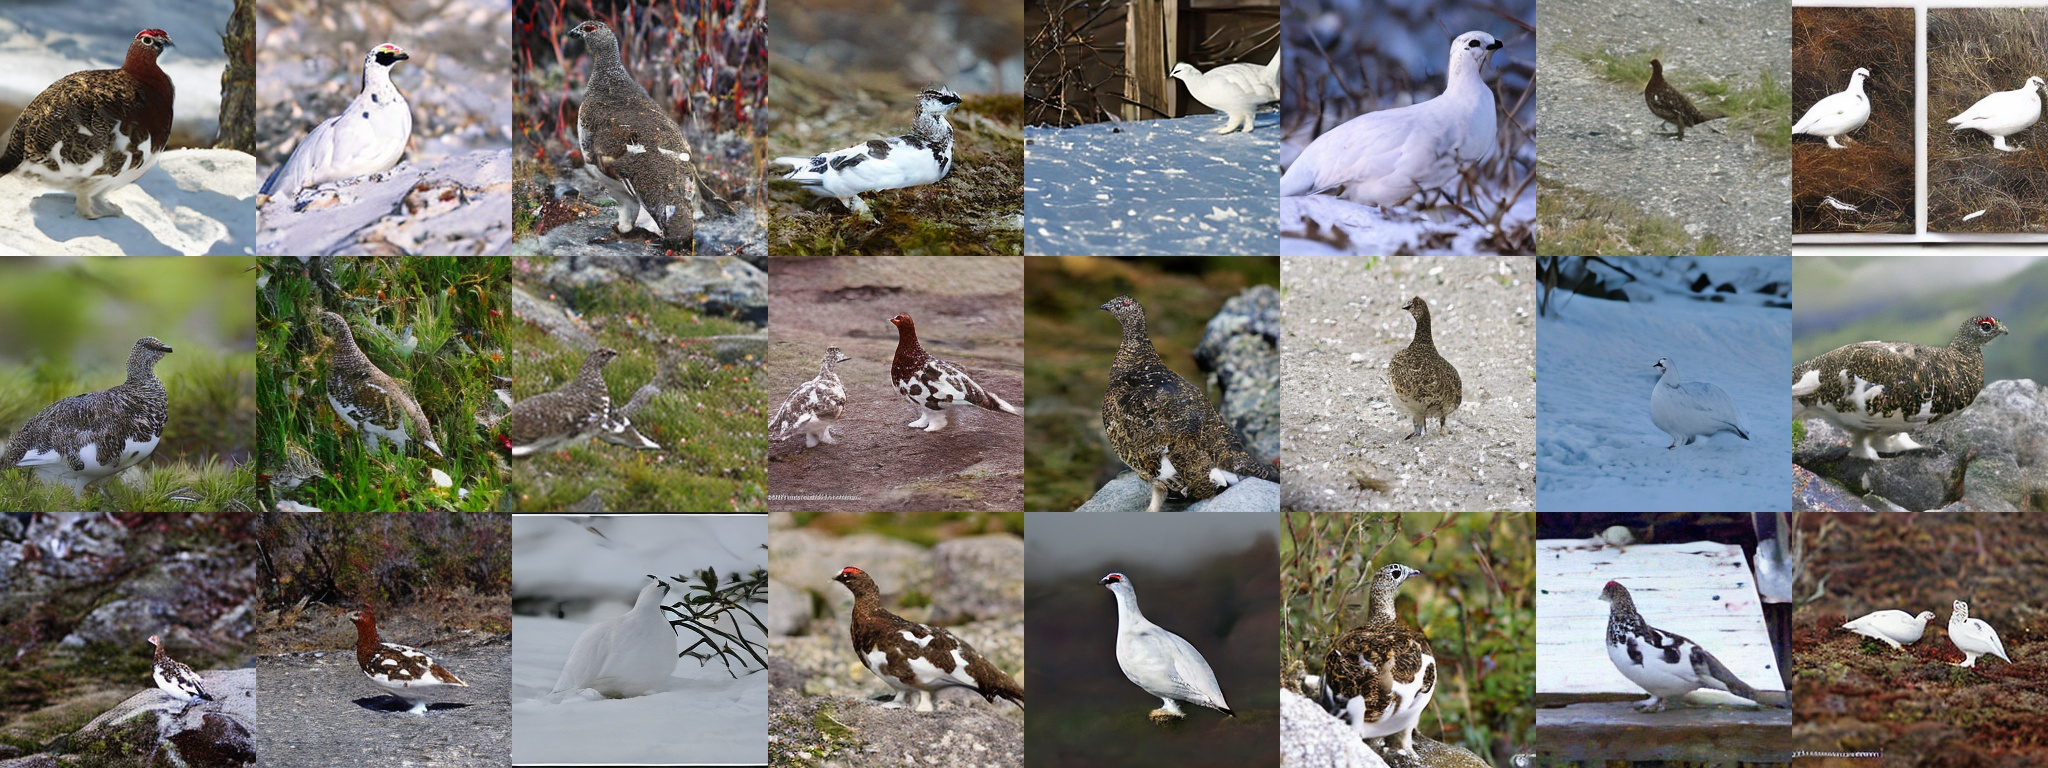
\includegraphics[width=\linewidth]{figures/imf_images/81.jpg}
    \end{minipage}\\[-0.2em]
    \centering\small Class 081: Ptarmigan
    
    \caption{\textbf{Side-by-side comparison with improved MeanFlow (iMF)~\cite{geng2025improved} (page 1/5).} Uncurated samples from our method (left) and iMF (right) on \textbf{all} ImageNet classes visualized in the iMF paper. Both methods generate images with a single neural function evaluation (1-NFE). The iMF visualizations use CFG $\omega{=}6.0$ and interval $[t_\text{min}, t_\text{max}]{=}[0.2, 0.8]$, achieving FID 3.92 and IS 348.2 (DiT-XL/2). For fair comparison, we set the CFG scale to match the IS of iMF visualizations, which leads to FID 3.01 and IS 354.4 (at CFG=1.5) for our method (DiT-L/2).}
    \label{fig:comparison_imf_1}
\end{figure*}

\begin{figure*}[p]
    \centering
    % Header
    \begin{minipage}{0.48\textwidth}
        \centering{ours}
    \end{minipage}\hfill
    \begin{minipage}{0.48\textwidth}
        \centering{improved MeanFlow (iMF)}
    \end{minipage}\\[0.2em]
    
    % Class 108: Sea anemone
    \begin{minipage}[b]{0.48\textwidth}
        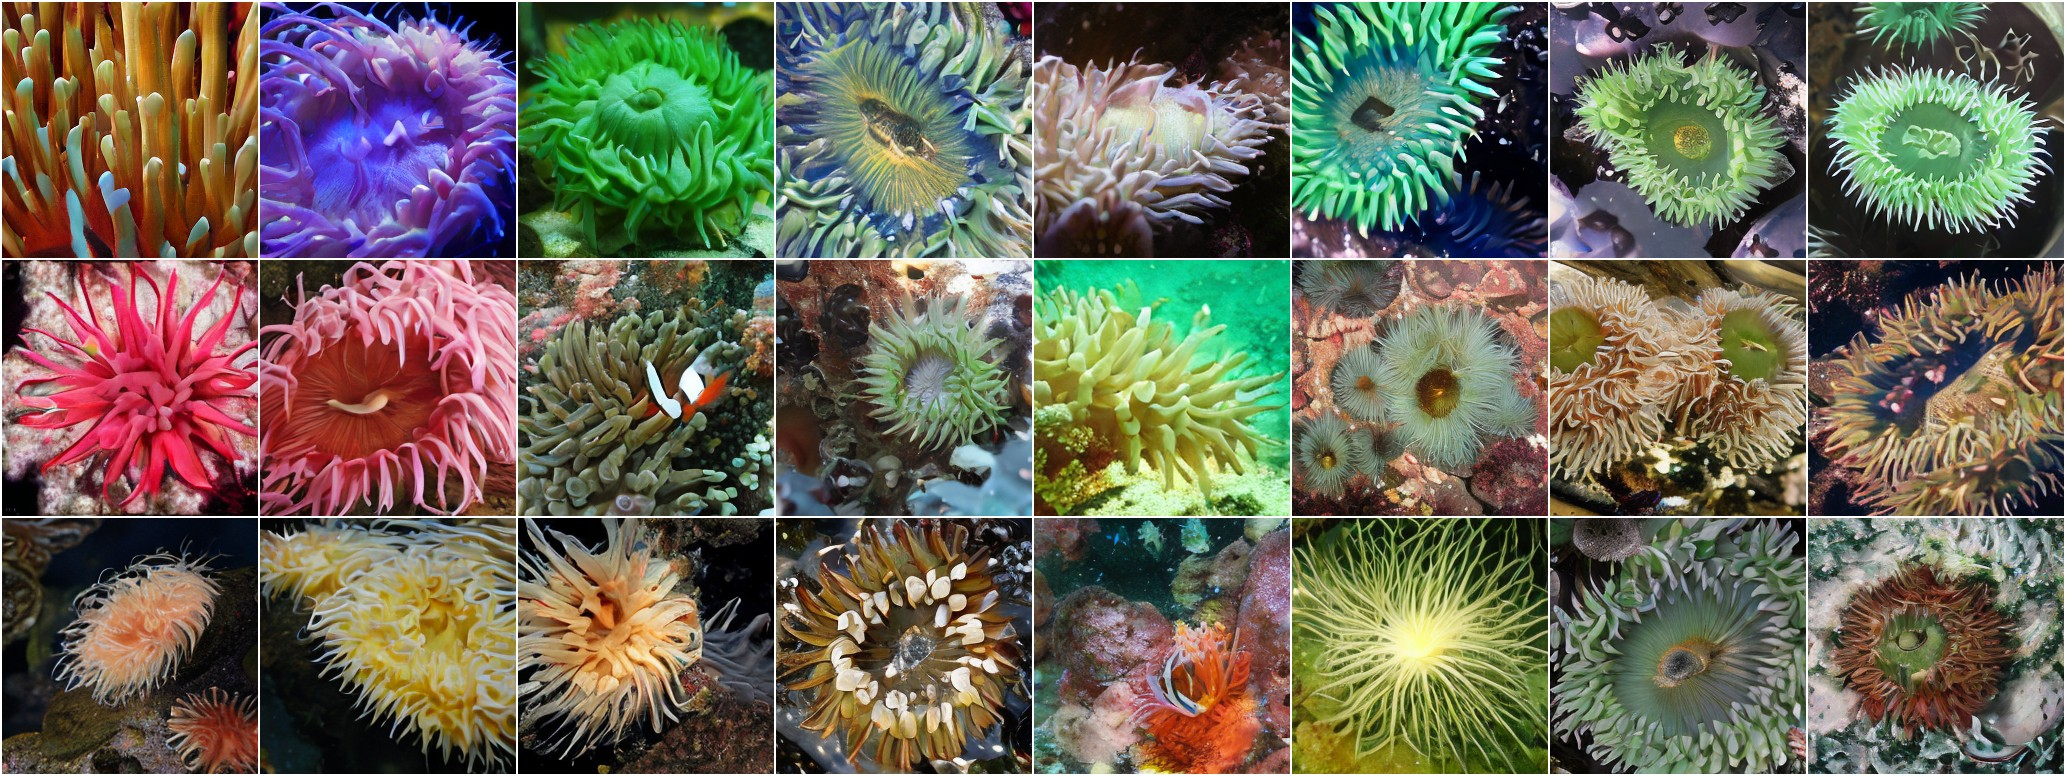
\includegraphics[width=\linewidth]{figures/imf_images/drift/classrank0175_class108_sea_anemone_score4.96.jpg}
    \end{minipage}\hfill
    \begin{minipage}[b]{0.48\textwidth}
        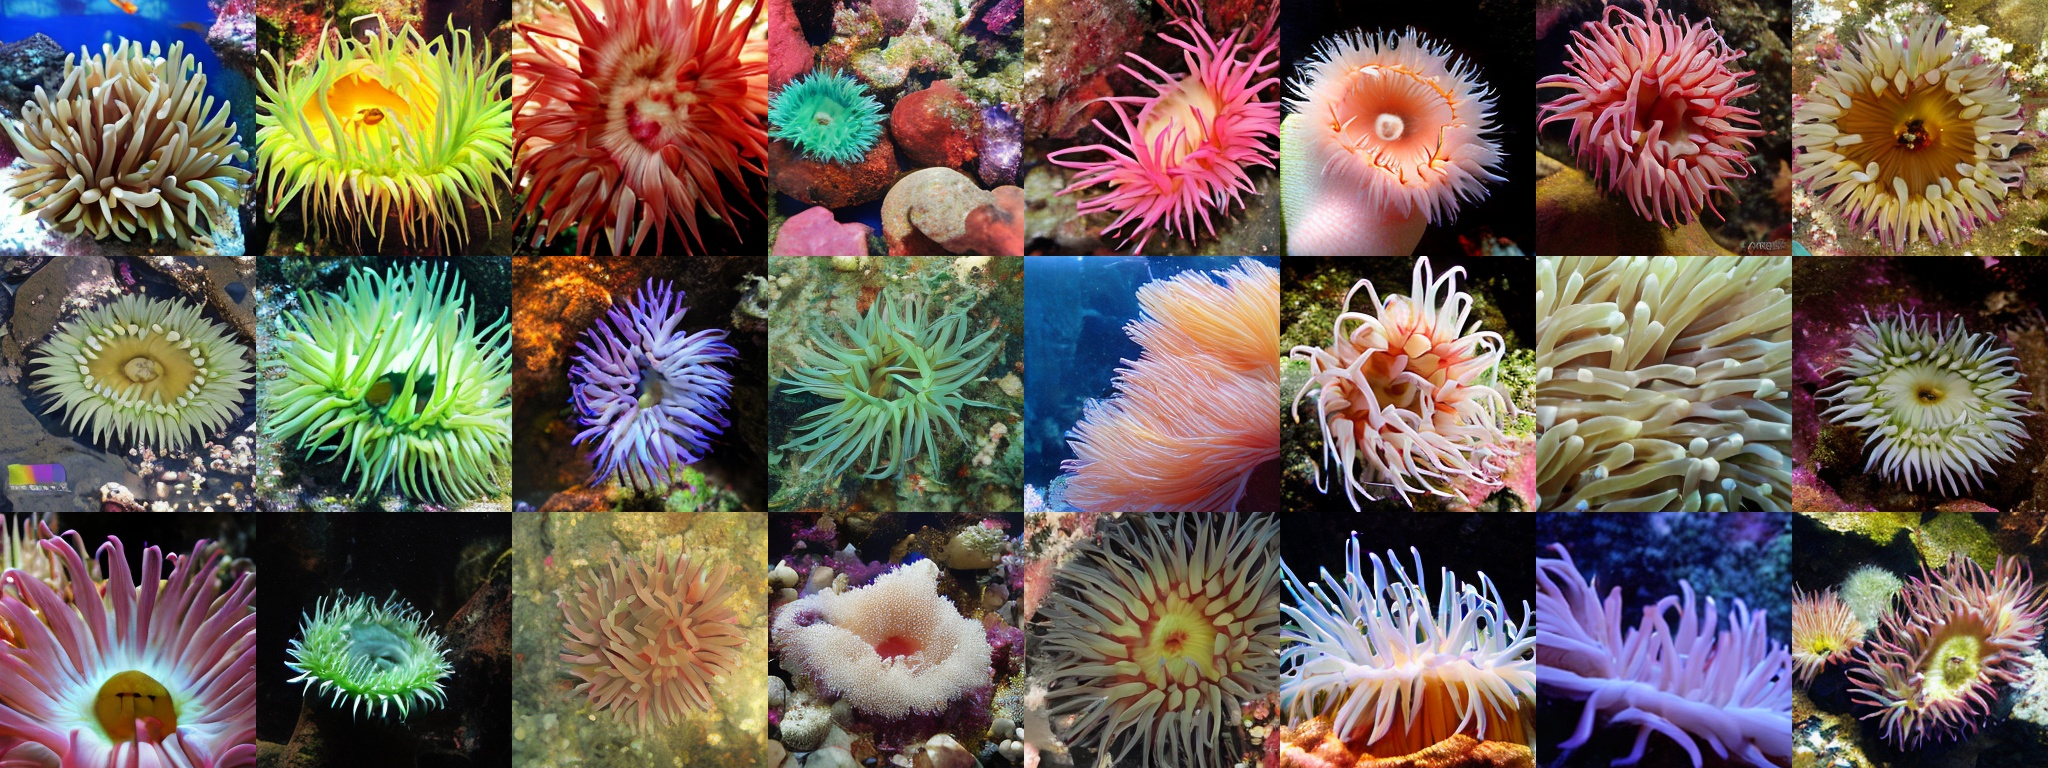
\includegraphics[width=\linewidth]{figures/imf_images/108.jpg}
    \end{minipage}\\[-0.2em]
    \centering\small Class 108: Sea anemone\\[0.2em]
    
    % Class 140: Red-backed sandpiper
    \begin{minipage}[b]{0.48\textwidth}
        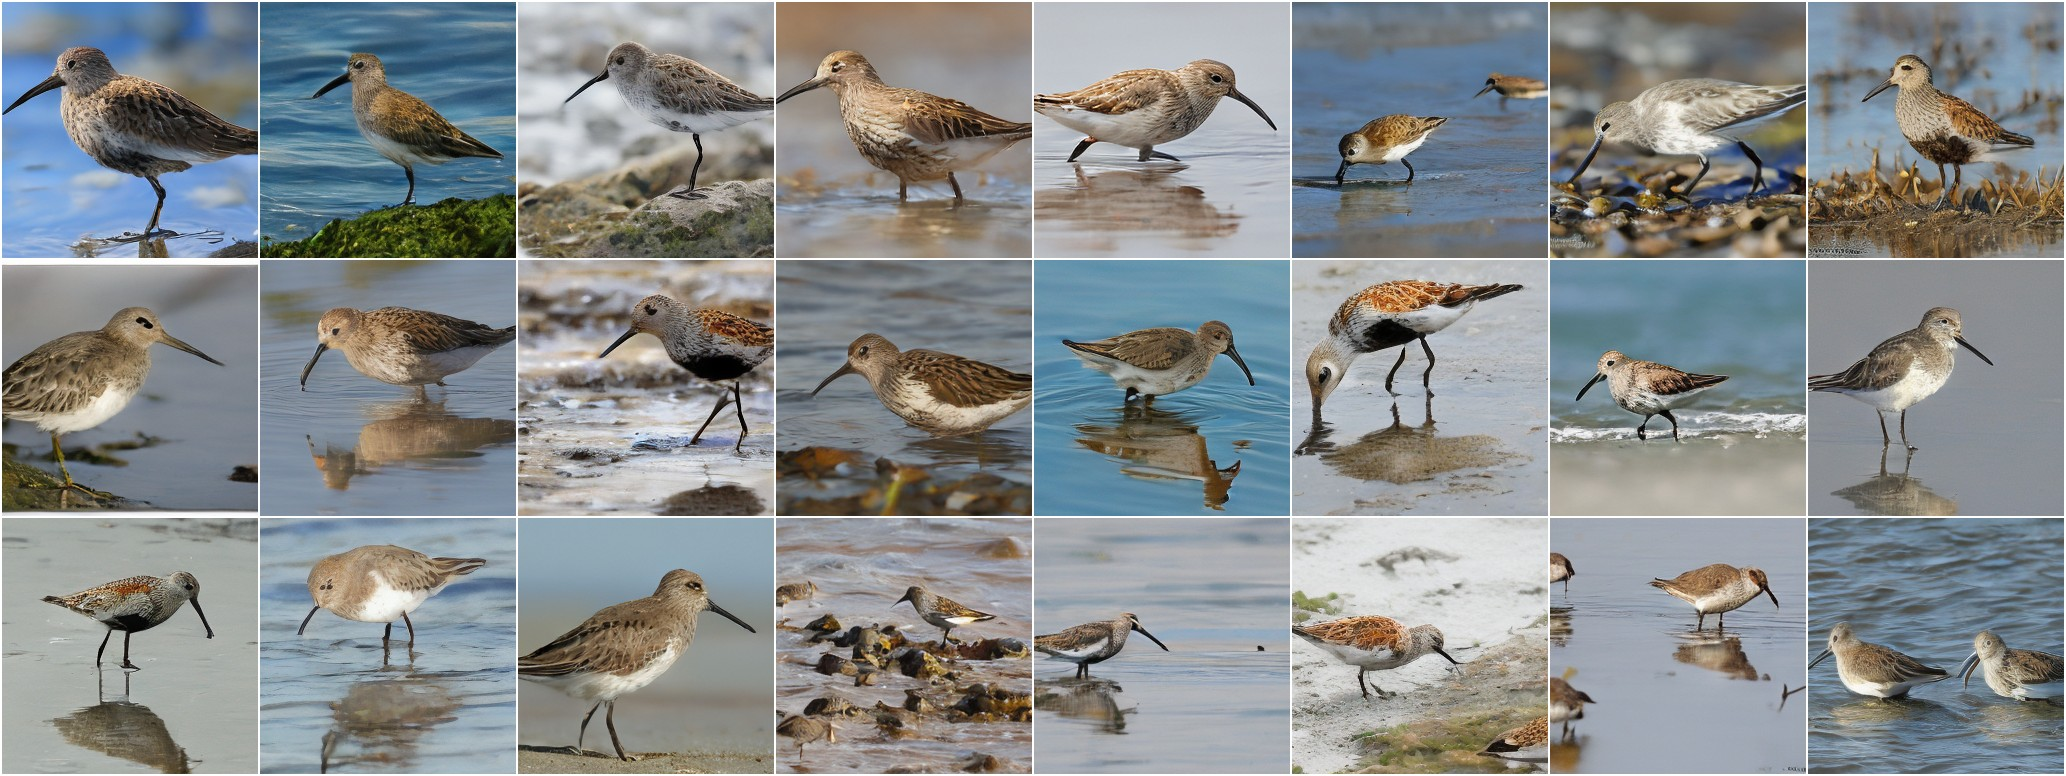
\includegraphics[width=\linewidth]{figures/imf_images/drift/classrank0011_class140_red_backed_sandpiper_score5.36.jpg}
    \end{minipage}\hfill
    \begin{minipage}[b]{0.48\textwidth}
        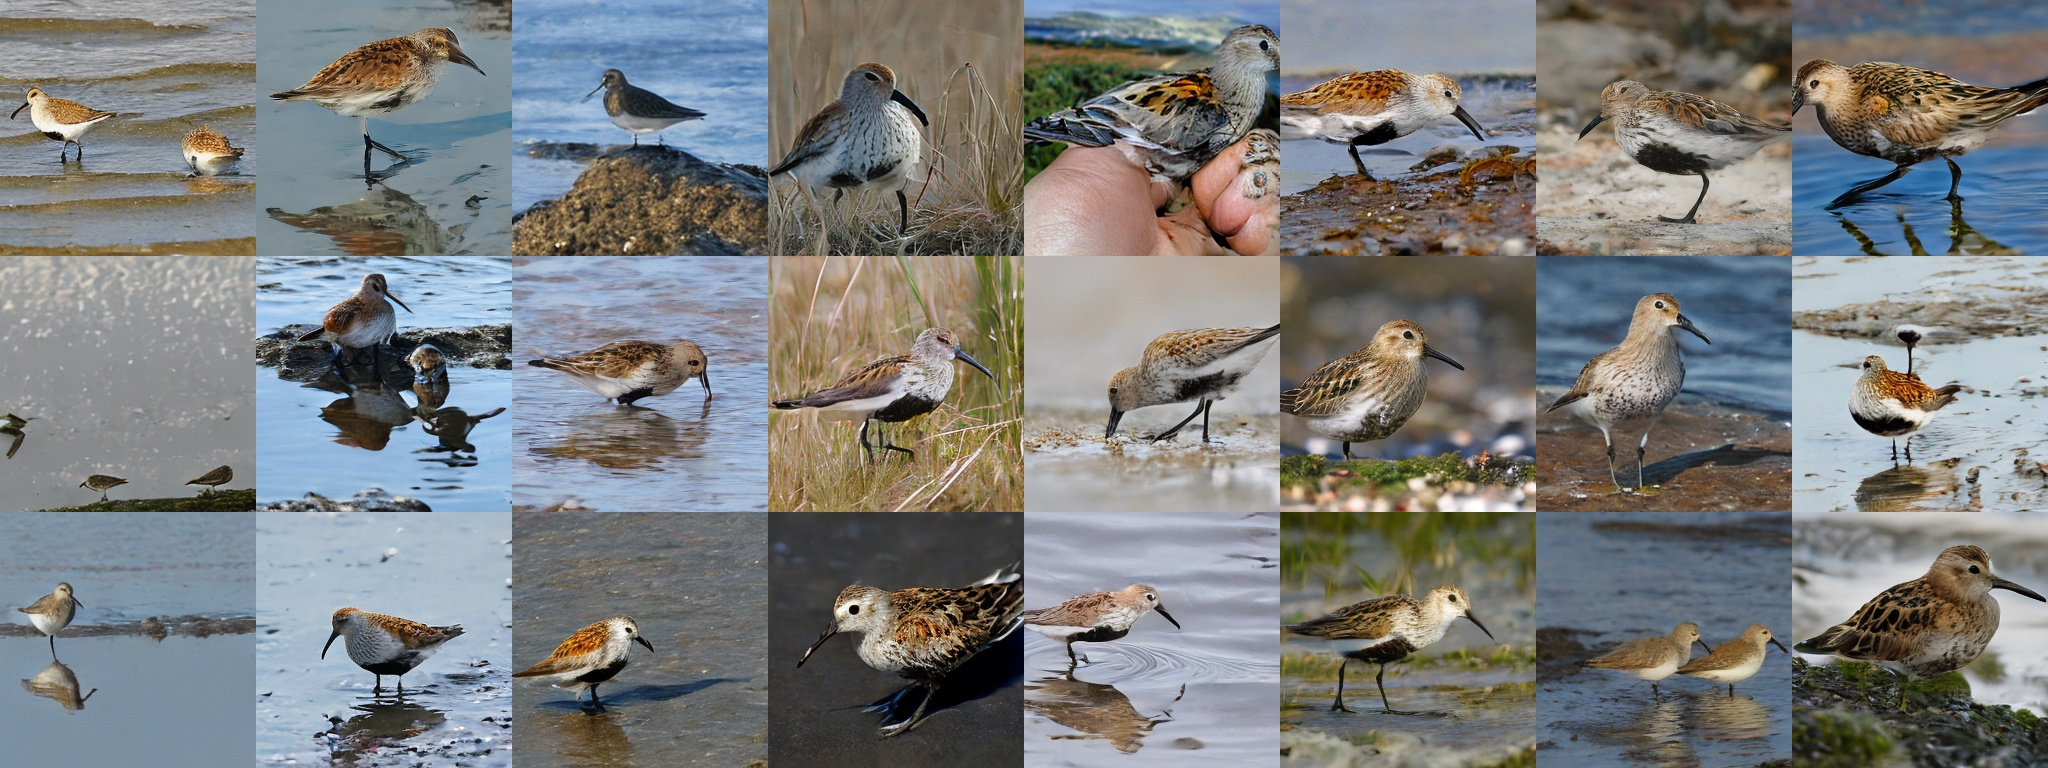
\includegraphics[width=\linewidth]{figures/imf_images/140.jpg}
    \end{minipage}\\[-0.2em]
    \centering\small Class 140: Red-backed sandpiper\\[0.2em]
    
    % Class 289: Snow leopard
    \begin{minipage}[b]{0.48\textwidth}
        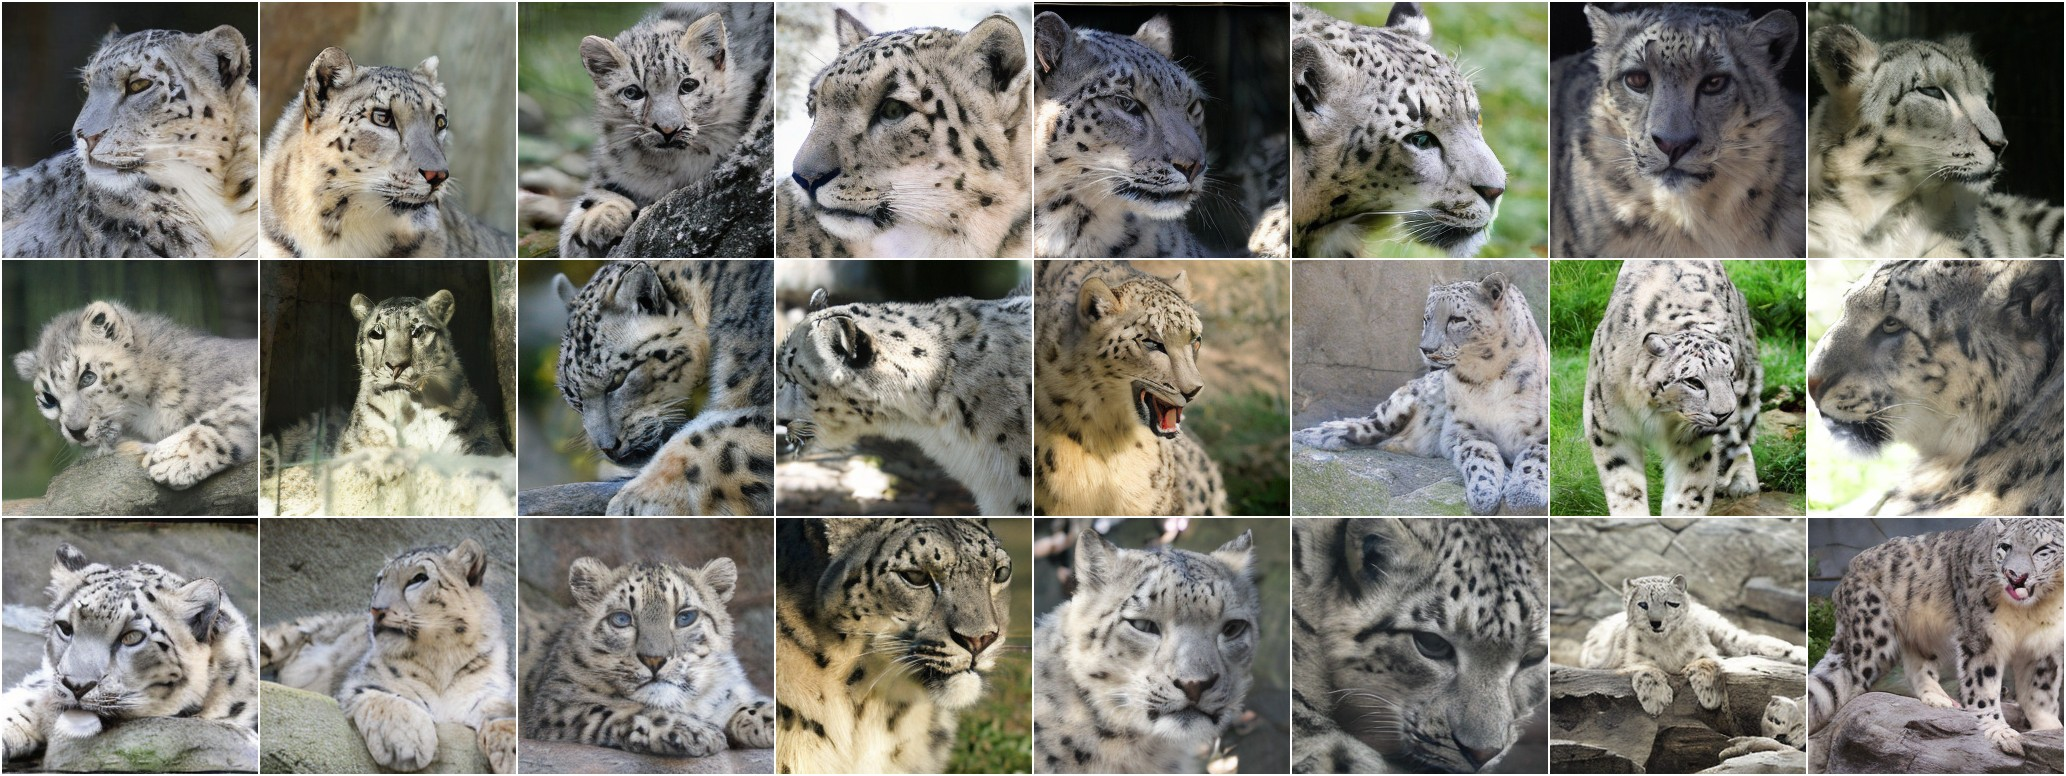
\includegraphics[width=\linewidth]{figures/imf_images/drift/classrank0067_class289_snow_leopard_score5.13.jpg}
    \end{minipage}\hfill
    \begin{minipage}[b]{0.48\textwidth}
        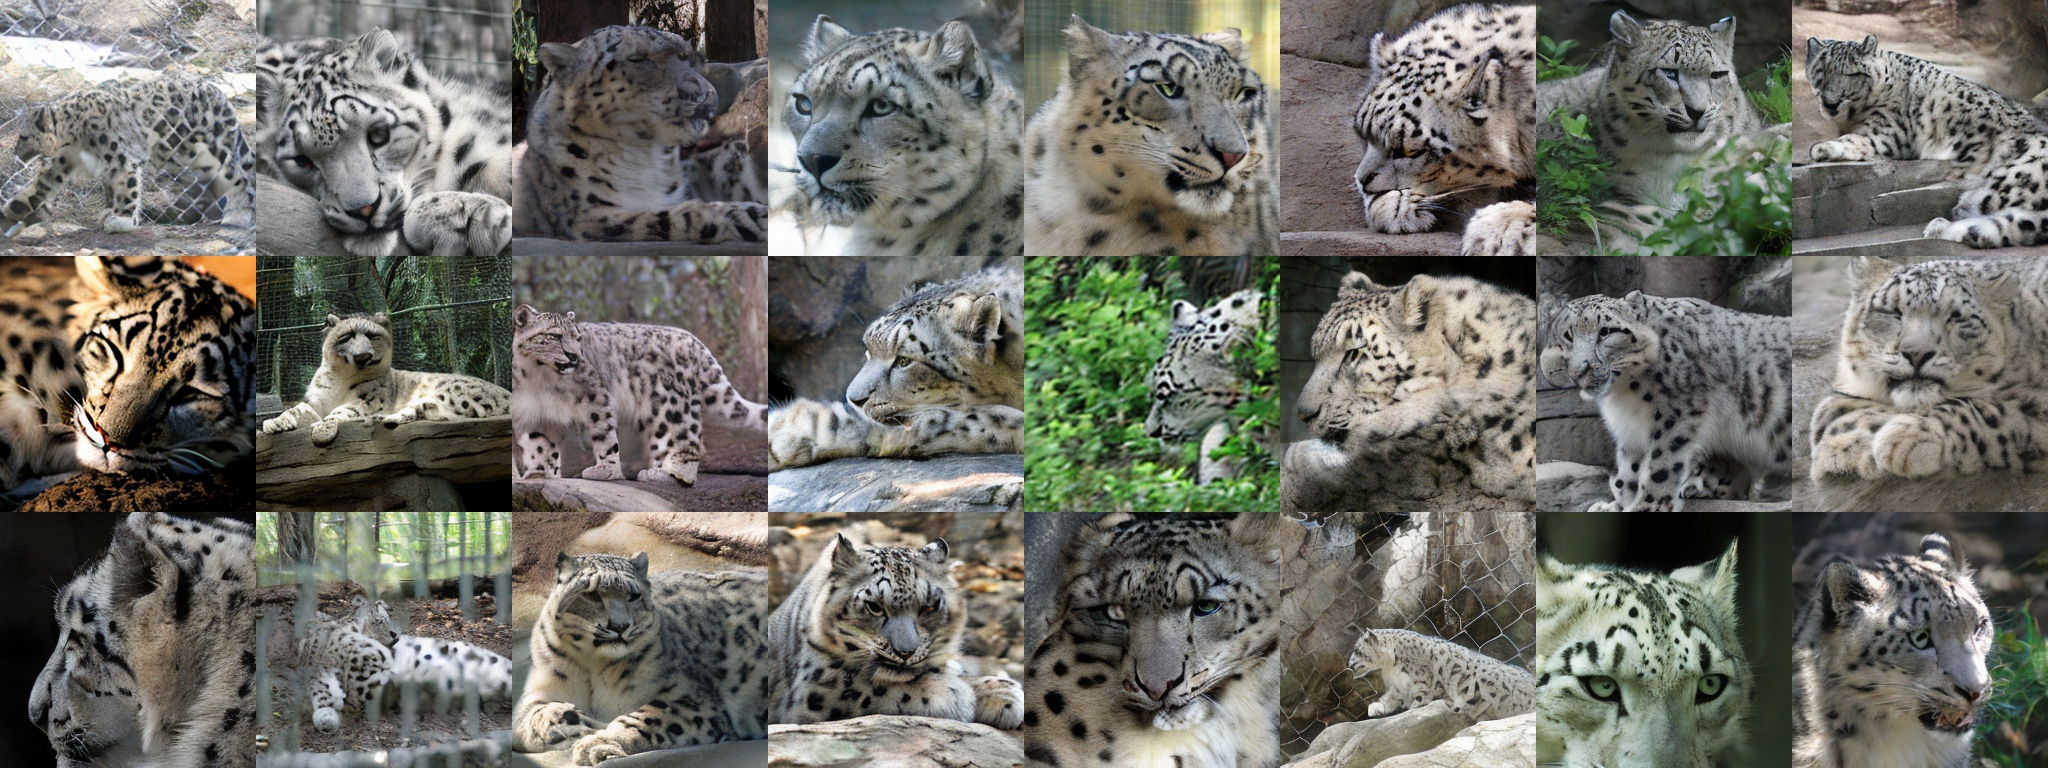
\includegraphics[width=\linewidth]{figures/imf_images/289.jpg}
    \end{minipage}\\[-0.2em]
    \centering\small Class 289: Snow leopard\\[0.2em]
    
    % Class 291: Lion
    \begin{minipage}[b]{0.48\textwidth}
        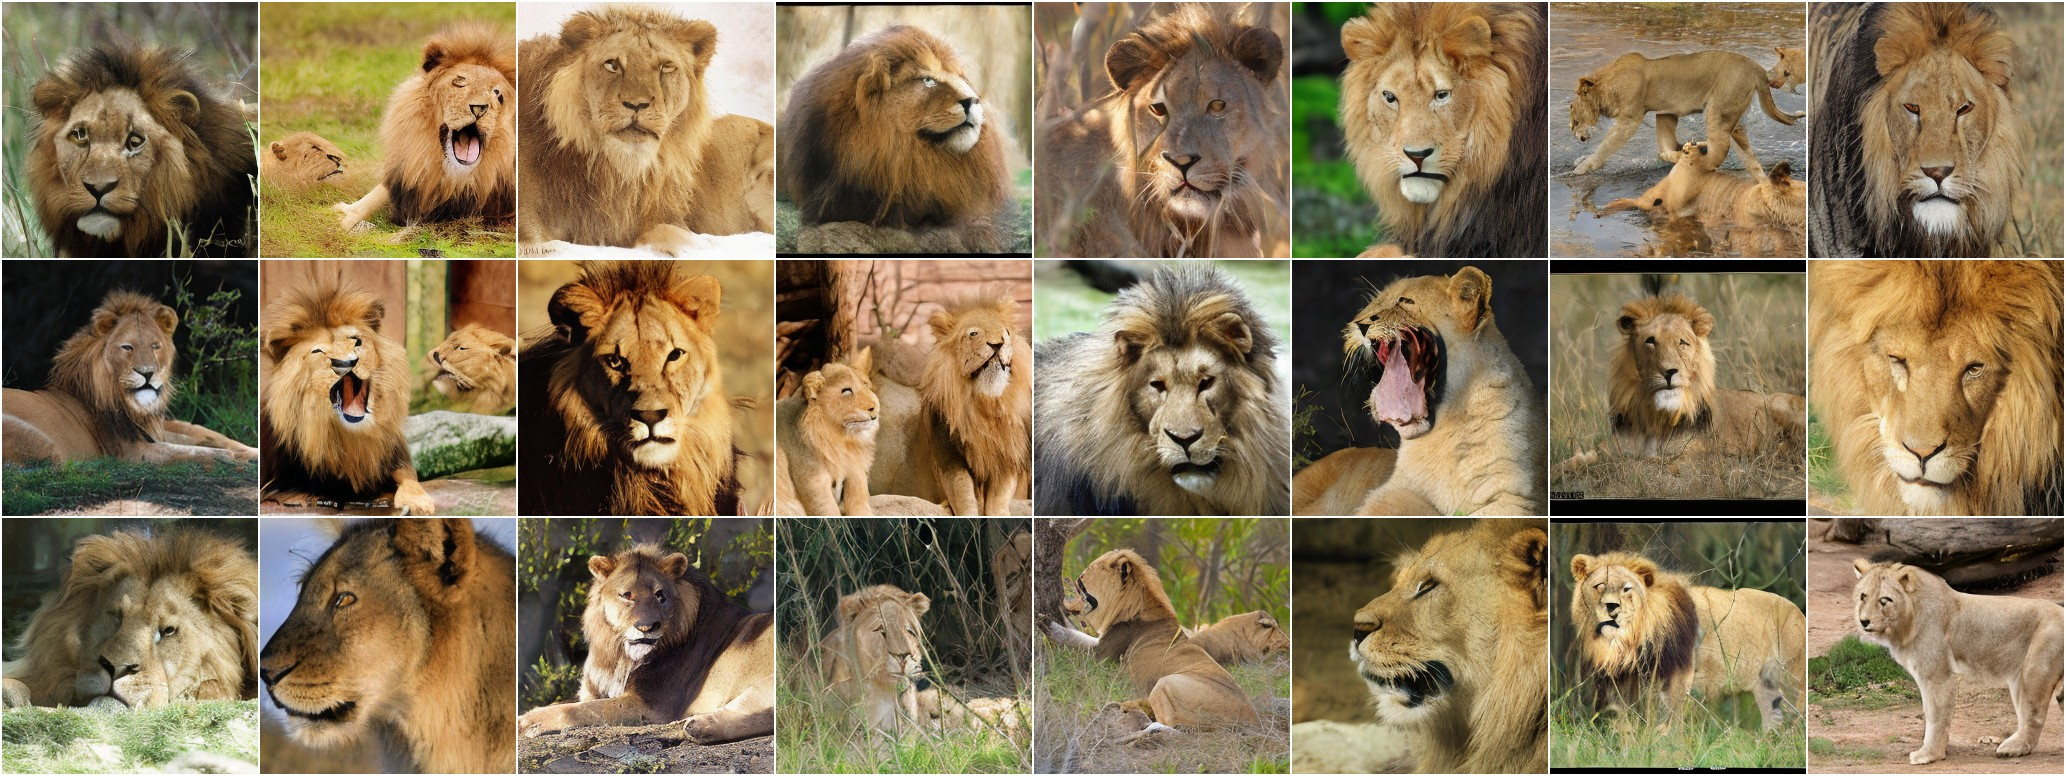
\includegraphics[width=\linewidth]{figures/imf_images/drift/classrank0069_class291_lion_score5.13.jpg}
    \end{minipage}\hfill
    \begin{minipage}[b]{0.48\textwidth}
        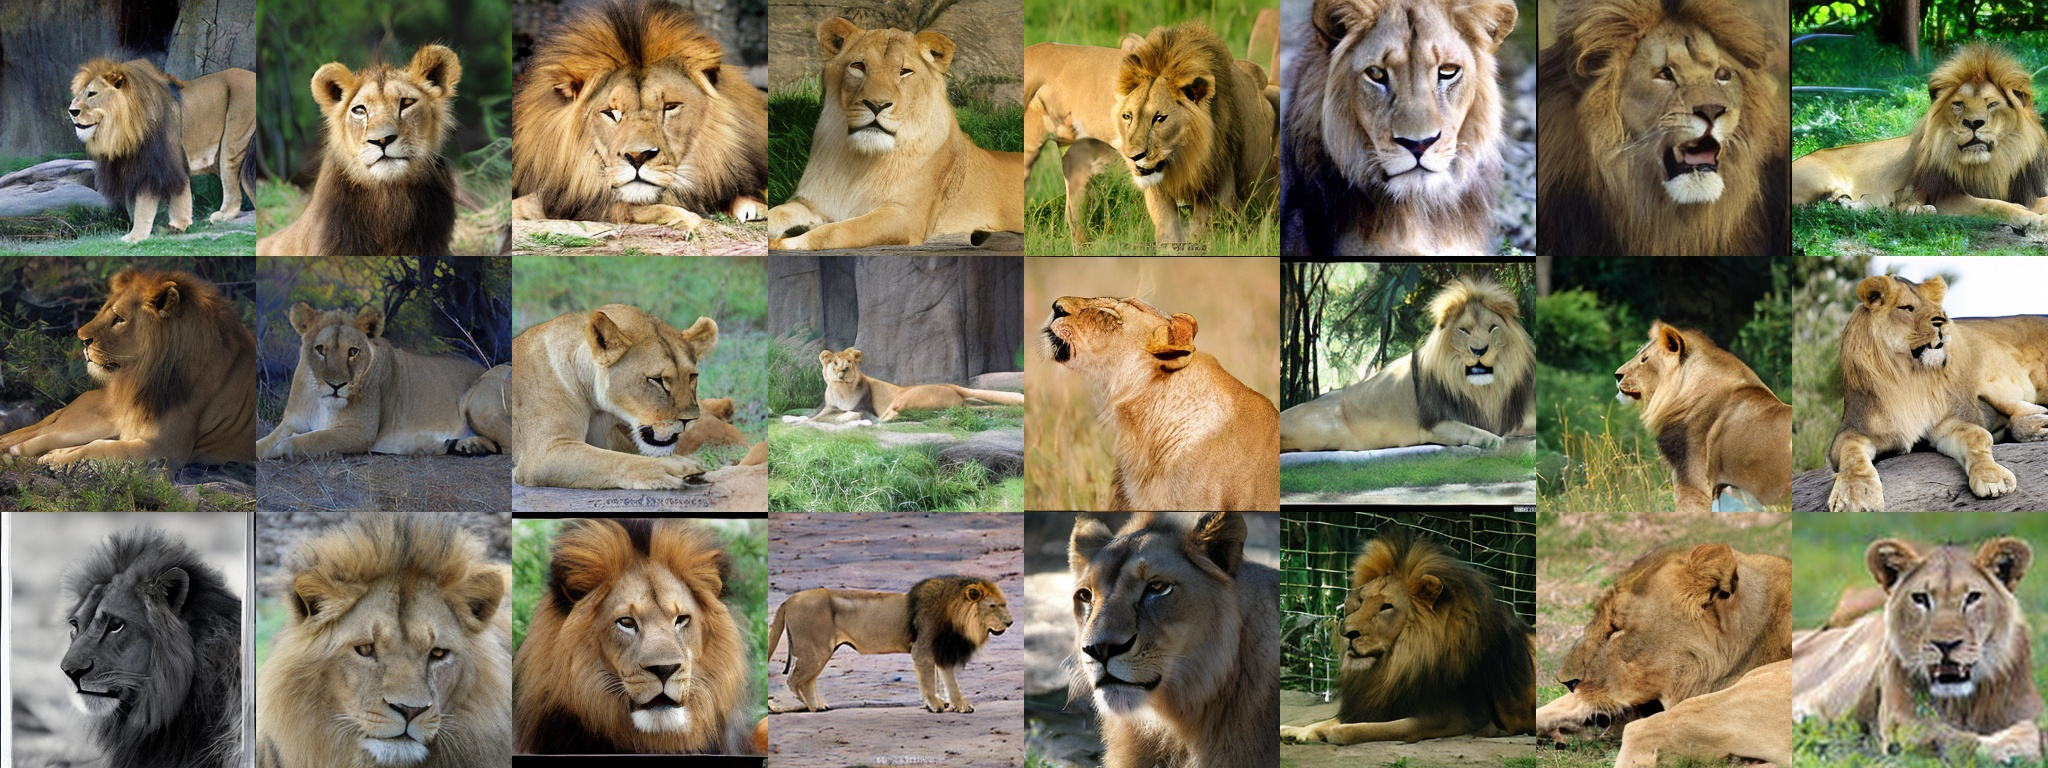
\includegraphics[width=\linewidth]{figures/imf_images/291.jpg}
    \end{minipage}\\[-0.2em]
    \centering\small Class 291: Lion\\[0.2em]
    
    % Class 387: Lesser panda
    \begin{minipage}[b]{0.48\textwidth}
        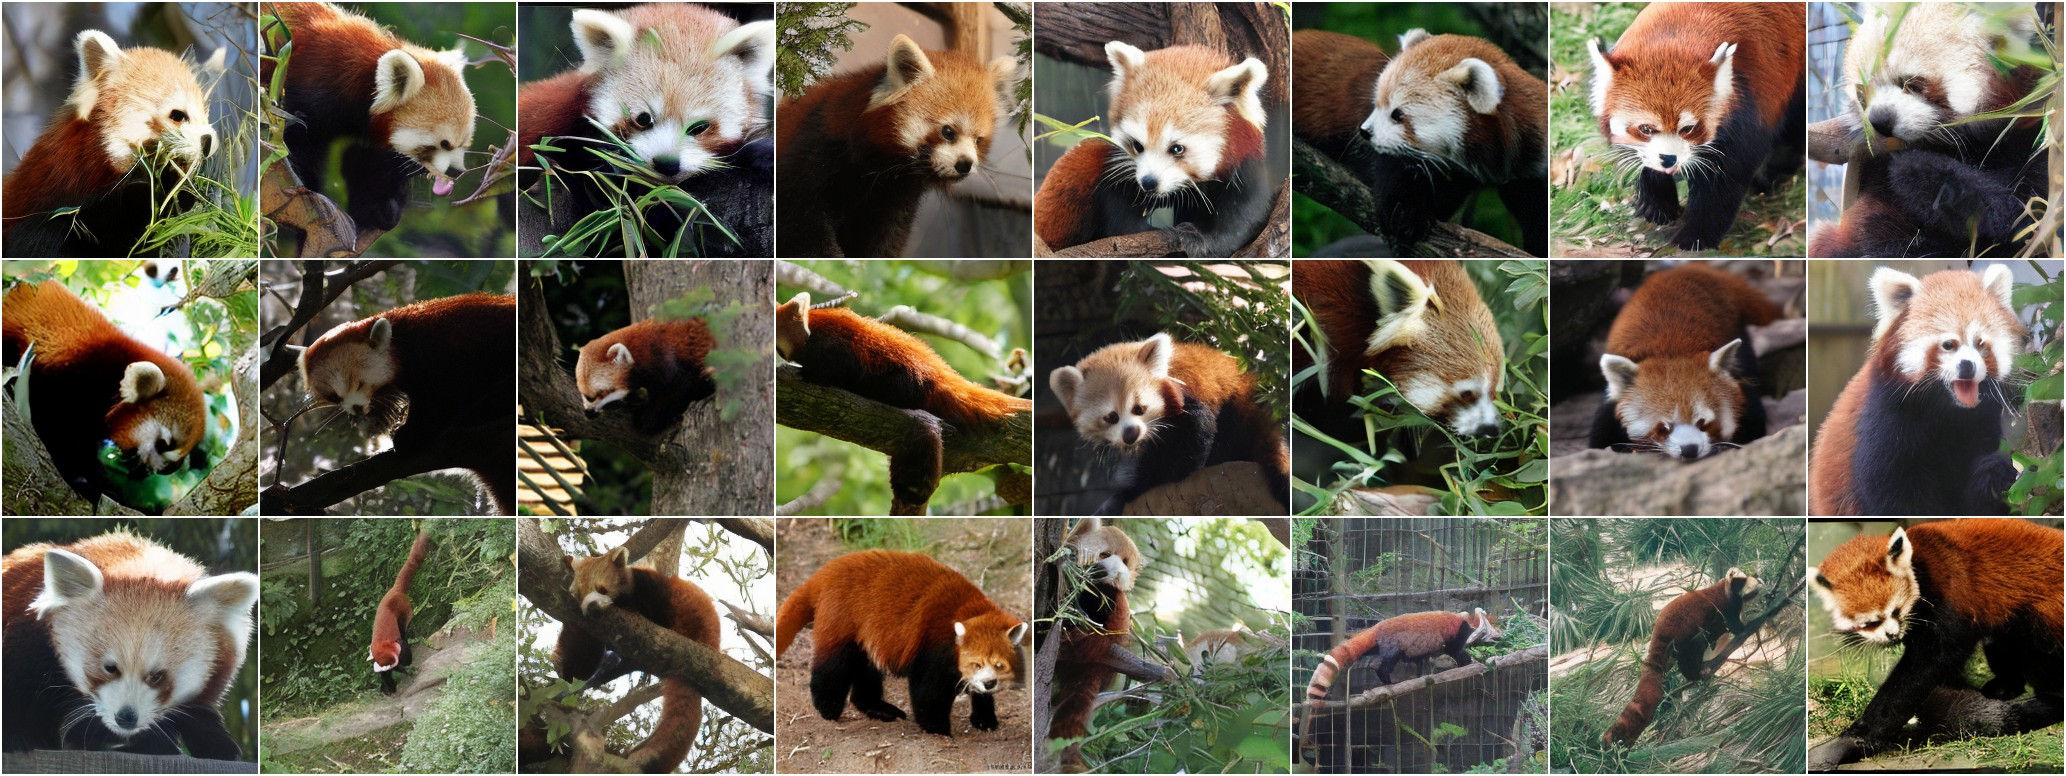
\includegraphics[width=\linewidth]{figures/imf_images/drift/classrank0243_class387_lesser_panda_score4.88.jpg}
    \end{minipage}\hfill
    \begin{minipage}[b]{0.48\textwidth}
        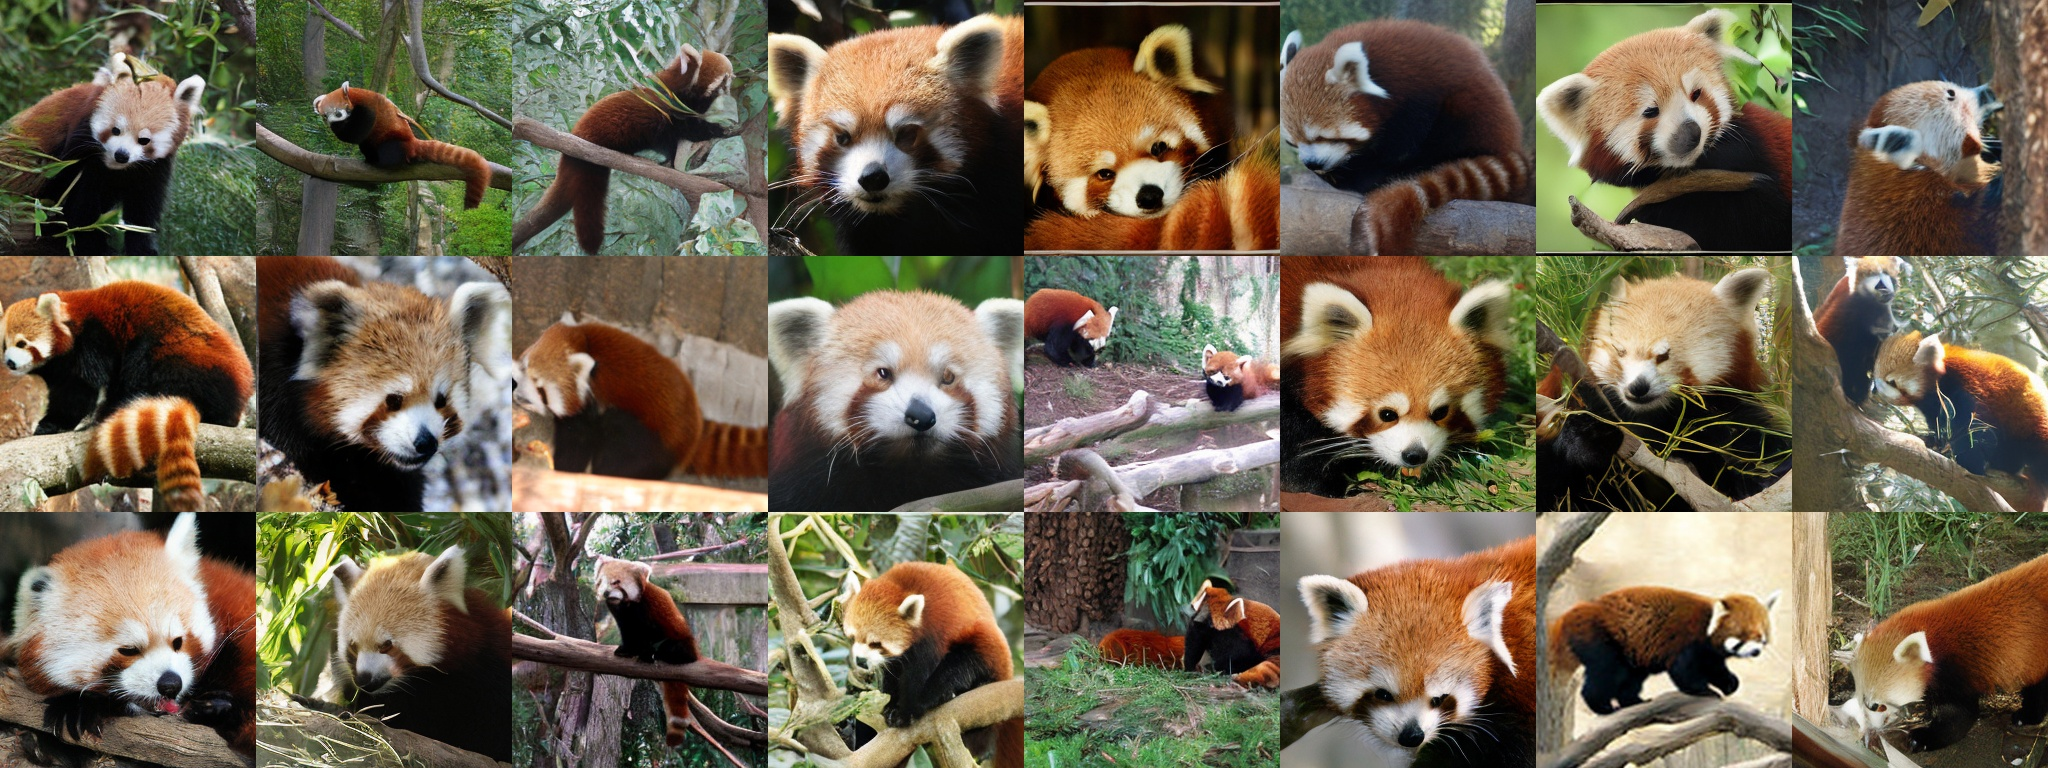
\includegraphics[width=\linewidth]{figures/imf_images/387.jpg}
    \end{minipage}\\[-0.2em]
    \centering\small Class 387: Lesser panda
    
    \caption{\textbf{Side-by-side comparison with improved MeanFlow (iMF)~\cite{geng2025improved} (page 2/5).} Uncurated samples from our method (left) and iMF (right) on \textbf{all} ImageNet classes visualized in the iMF paper. Both methods generate images with a single neural function evaluation (1-NFE). The iMF visualizations use CFG $\omega{=}6.0$ and interval $[t_\text{min}, t_\text{max}]{=}[0.2, 0.8]$, achieving FID 3.92 and IS 348.2 (DiT-XL/2). For fair comparison, we set the CFG scale to match the IS of iMF visualizations, which leads to FID 3.01 and IS 354.4 (at CFG=1.5) for our method (DiT-L/2).}
    \label{fig:comparison_imf_2}
\end{figure*}

\begin{figure*}[p]
    \centering
    % Header
    \begin{minipage}{0.48\textwidth}
        \centering{ours}
    \end{minipage}\hfill
    \begin{minipage}{0.48\textwidth}
        \centering{improved MeanFlow (iMF)}
    \end{minipage}\\[0.2em]
    
    % Class 437: Beacon
    \begin{minipage}[b]{0.48\textwidth}
        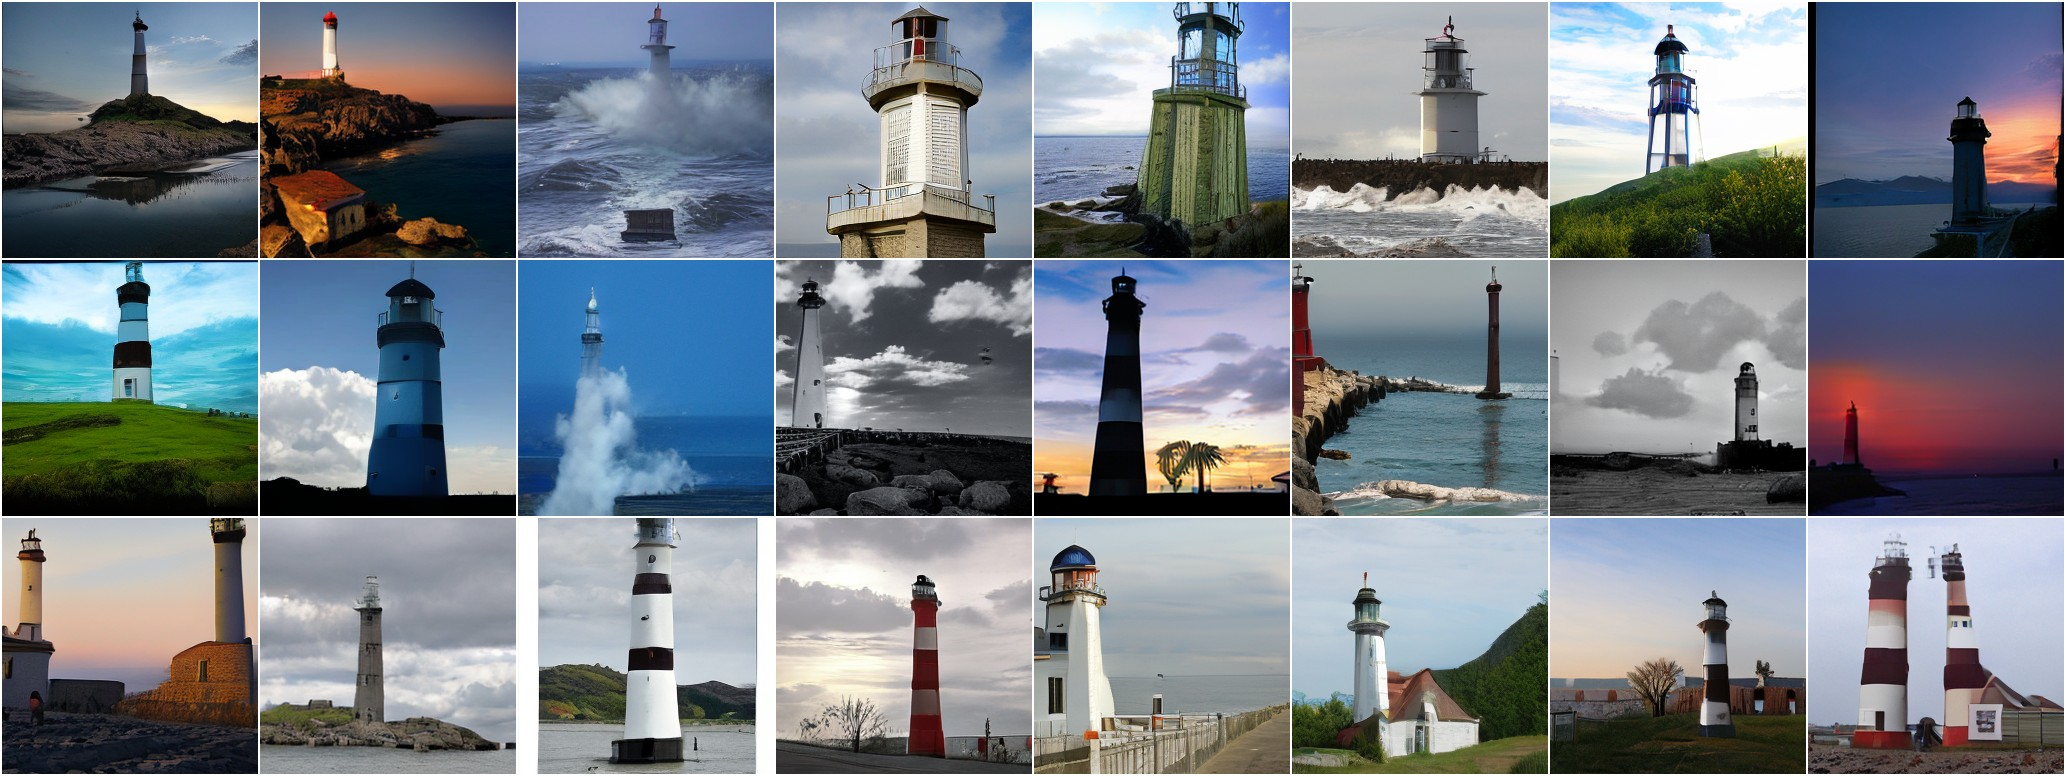
\includegraphics[width=\linewidth]{figures/imf_images/drift/classrank0076_class437_beacon_score5.11.jpg}
    \end{minipage}\hfill
    \begin{minipage}[b]{0.48\textwidth}
        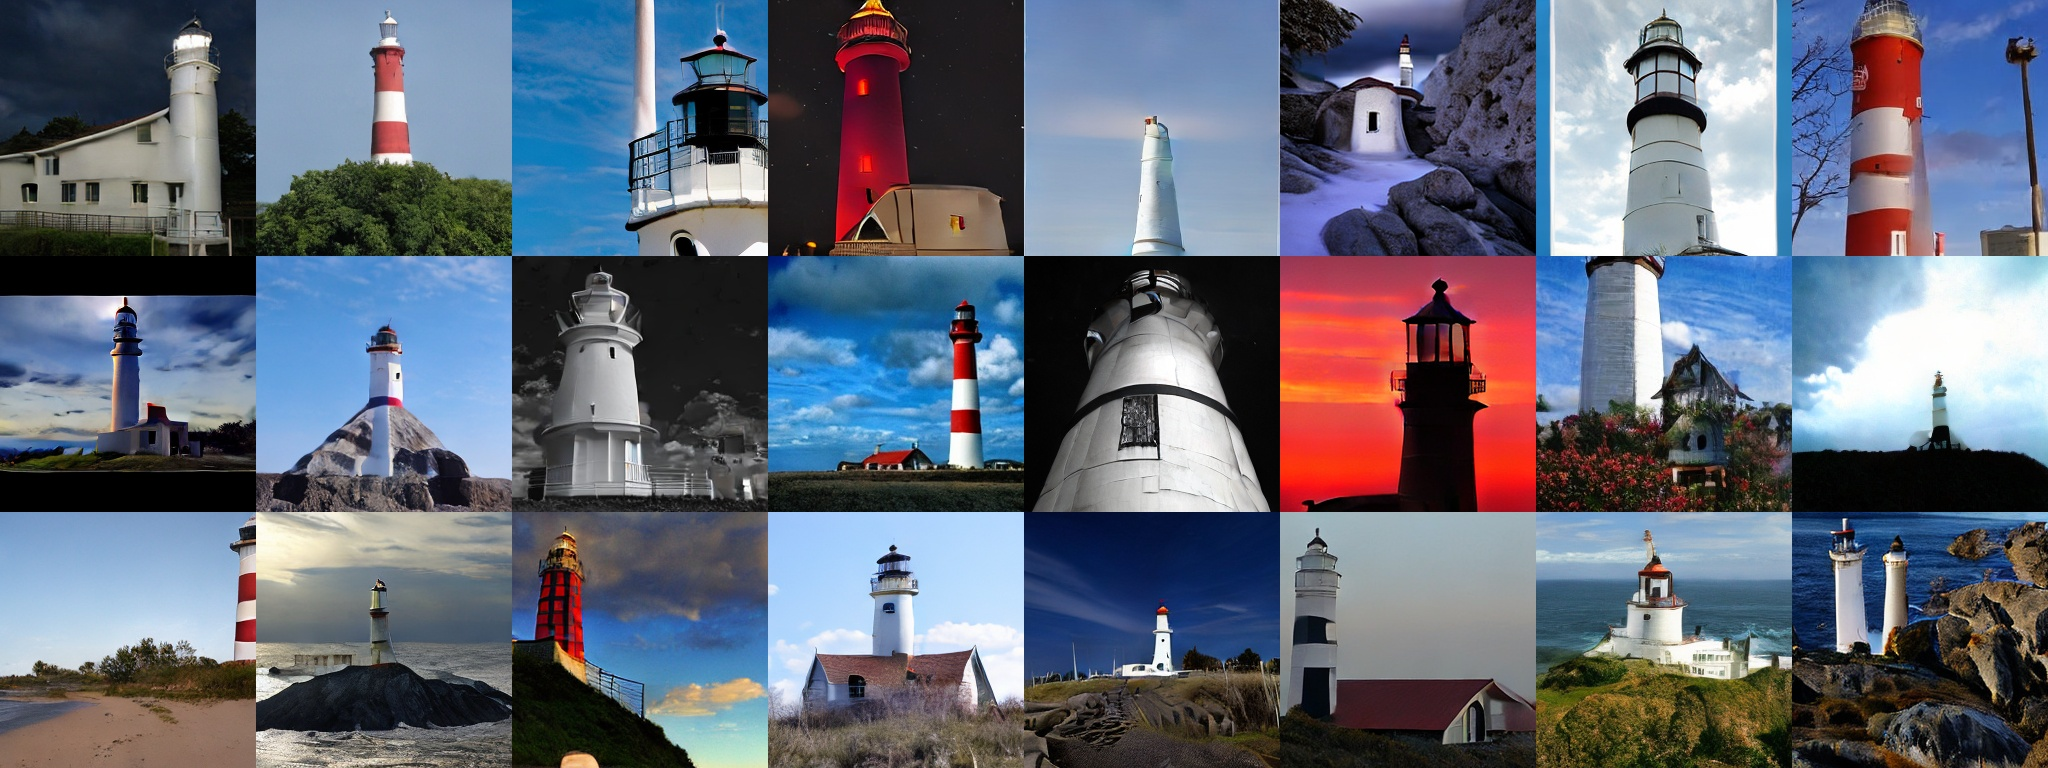
\includegraphics[width=\linewidth]{figures/imf_images/437.jpg}
    \end{minipage}\\[-0.2em]
    \centering\small Class 437: Beacon\\[0.2em]
    
    % Class 483: Castle
    \begin{minipage}[b]{0.48\textwidth}
        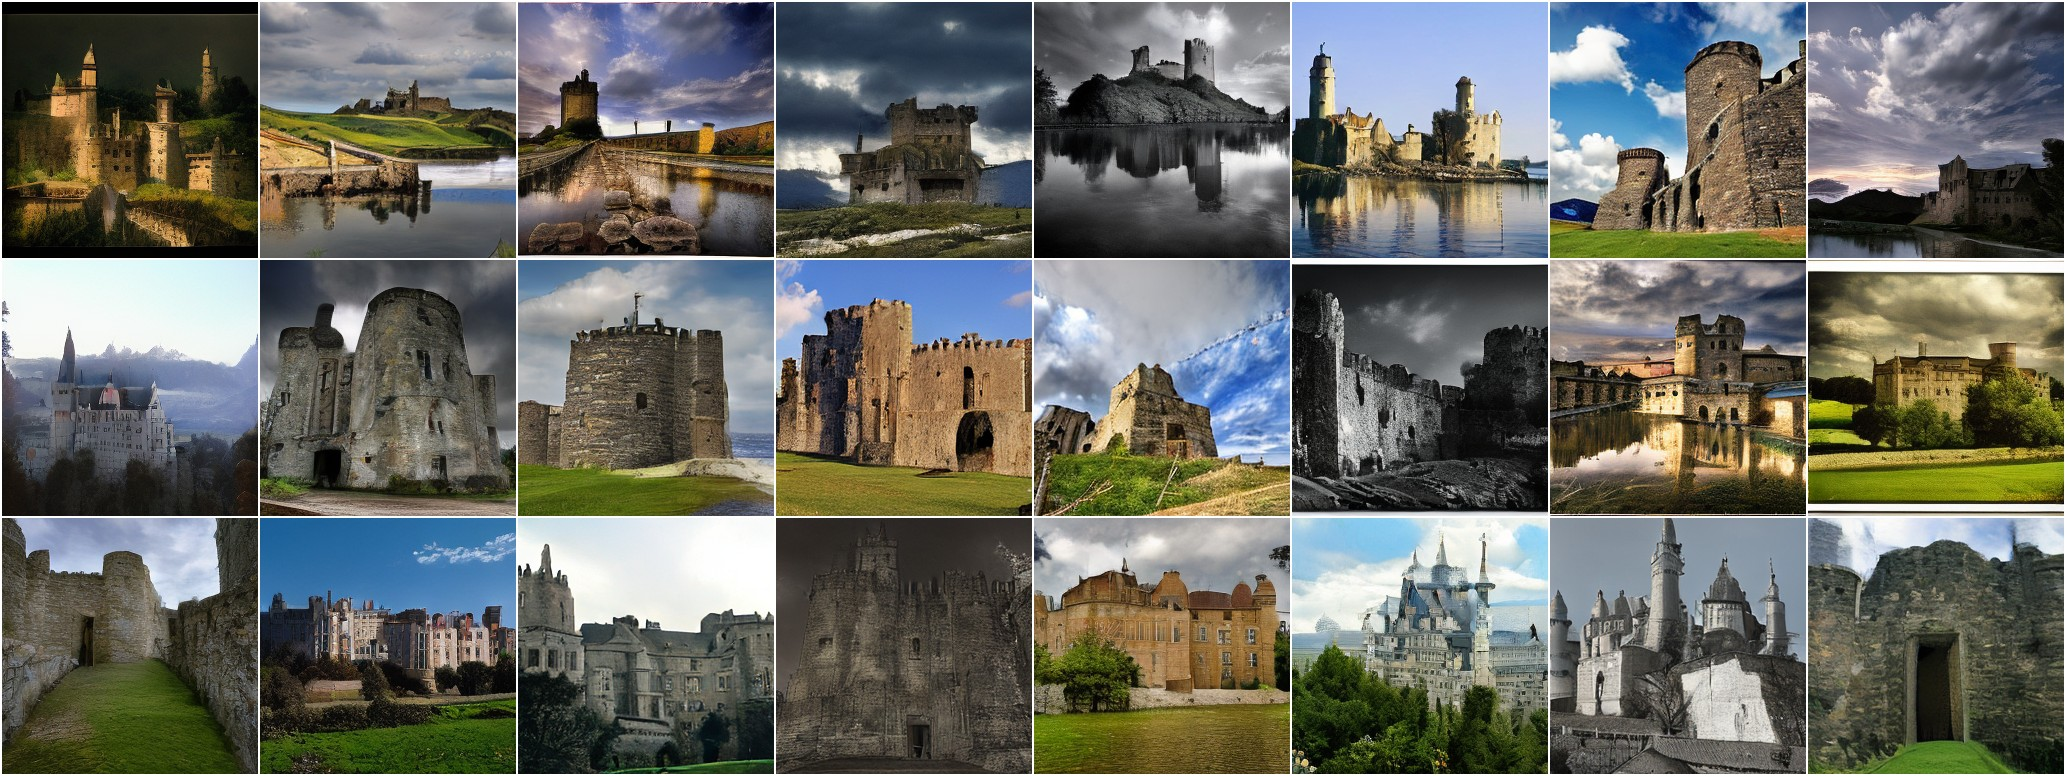
\includegraphics[width=\linewidth]{figures/imf_images/drift/classrank0000_class483_castle_score5.50.jpg}
    \end{minipage}\hfill
    \begin{minipage}[b]{0.48\textwidth}
        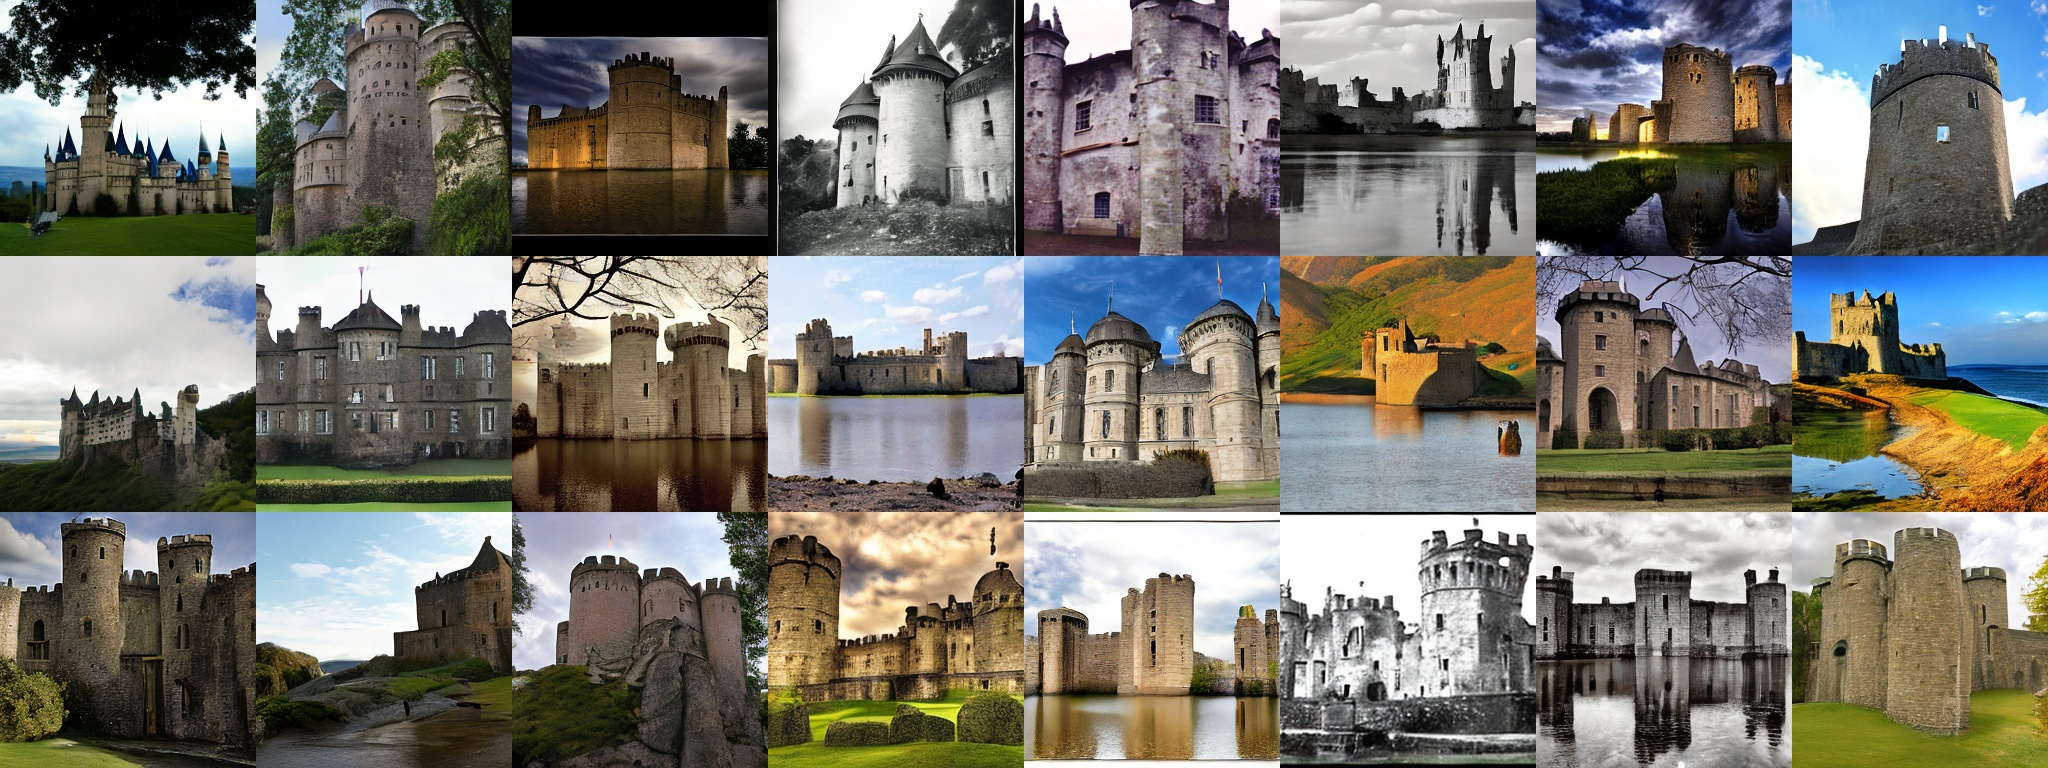
\includegraphics[width=\linewidth]{figures/imf_images/483.jpg}
    \end{minipage}\\[-0.2em]
    \centering\small Class 483: Castle\\[0.2em]
    
    % Class 540: Drilling platform
    \begin{minipage}[b]{0.48\textwidth}
        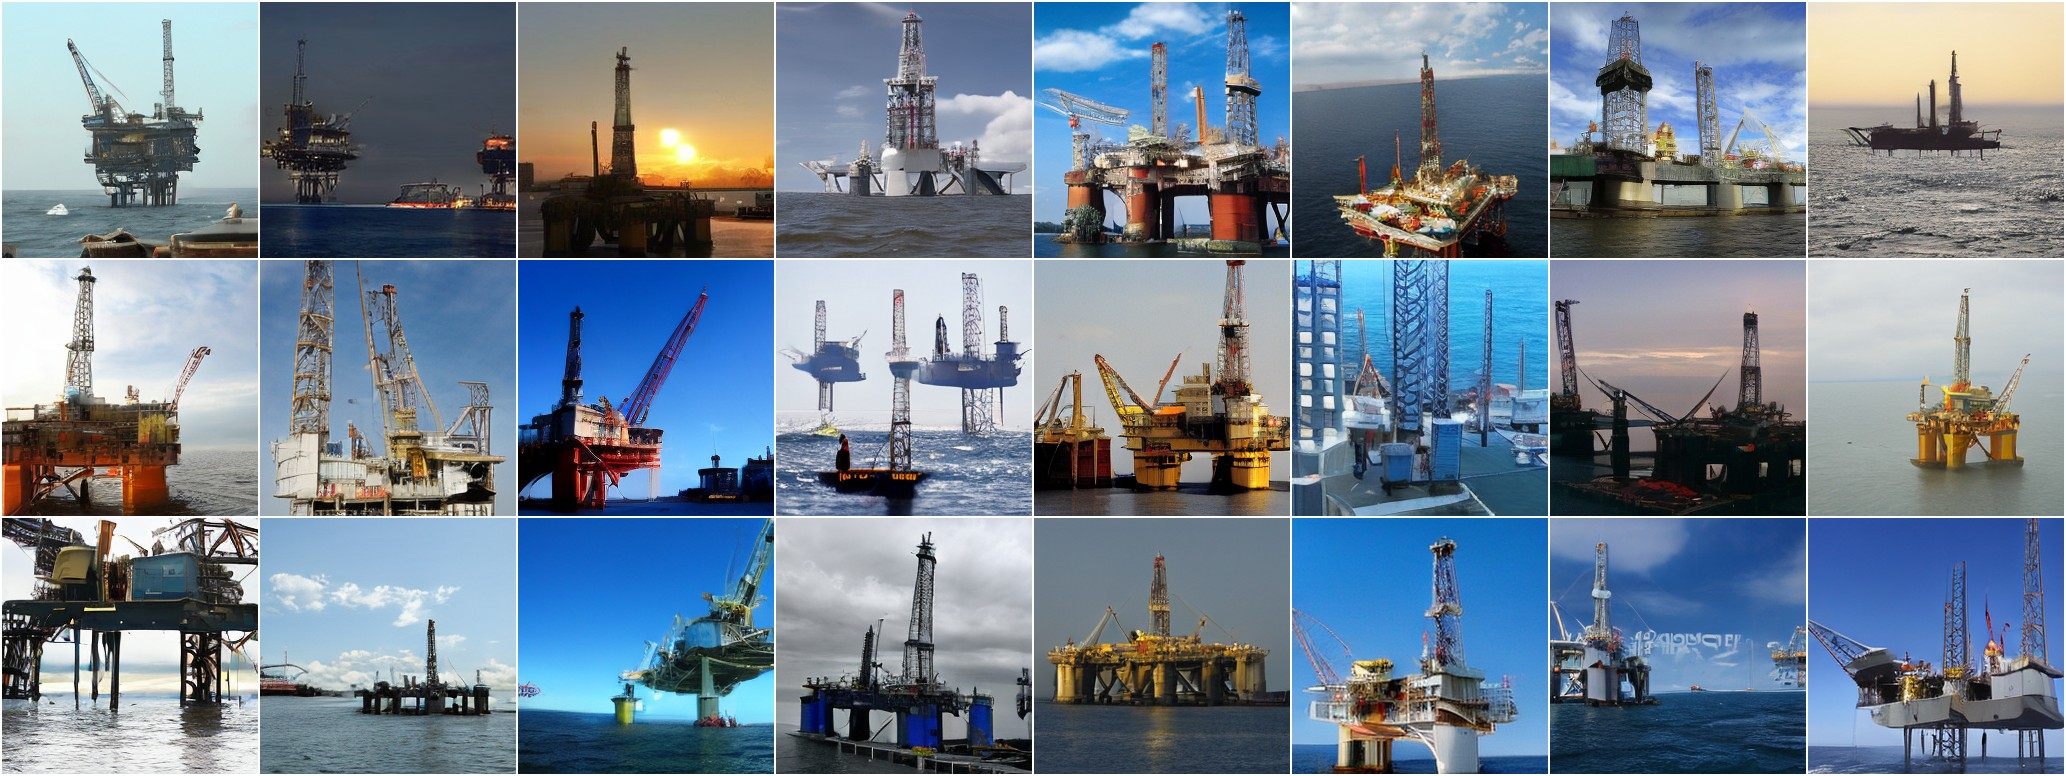
\includegraphics[width=\linewidth]{figures/imf_images/drift/classrank0352_class540_drilling_platform_score4.77.jpg}
    \end{minipage}\hfill
    \begin{minipage}[b]{0.48\textwidth}
        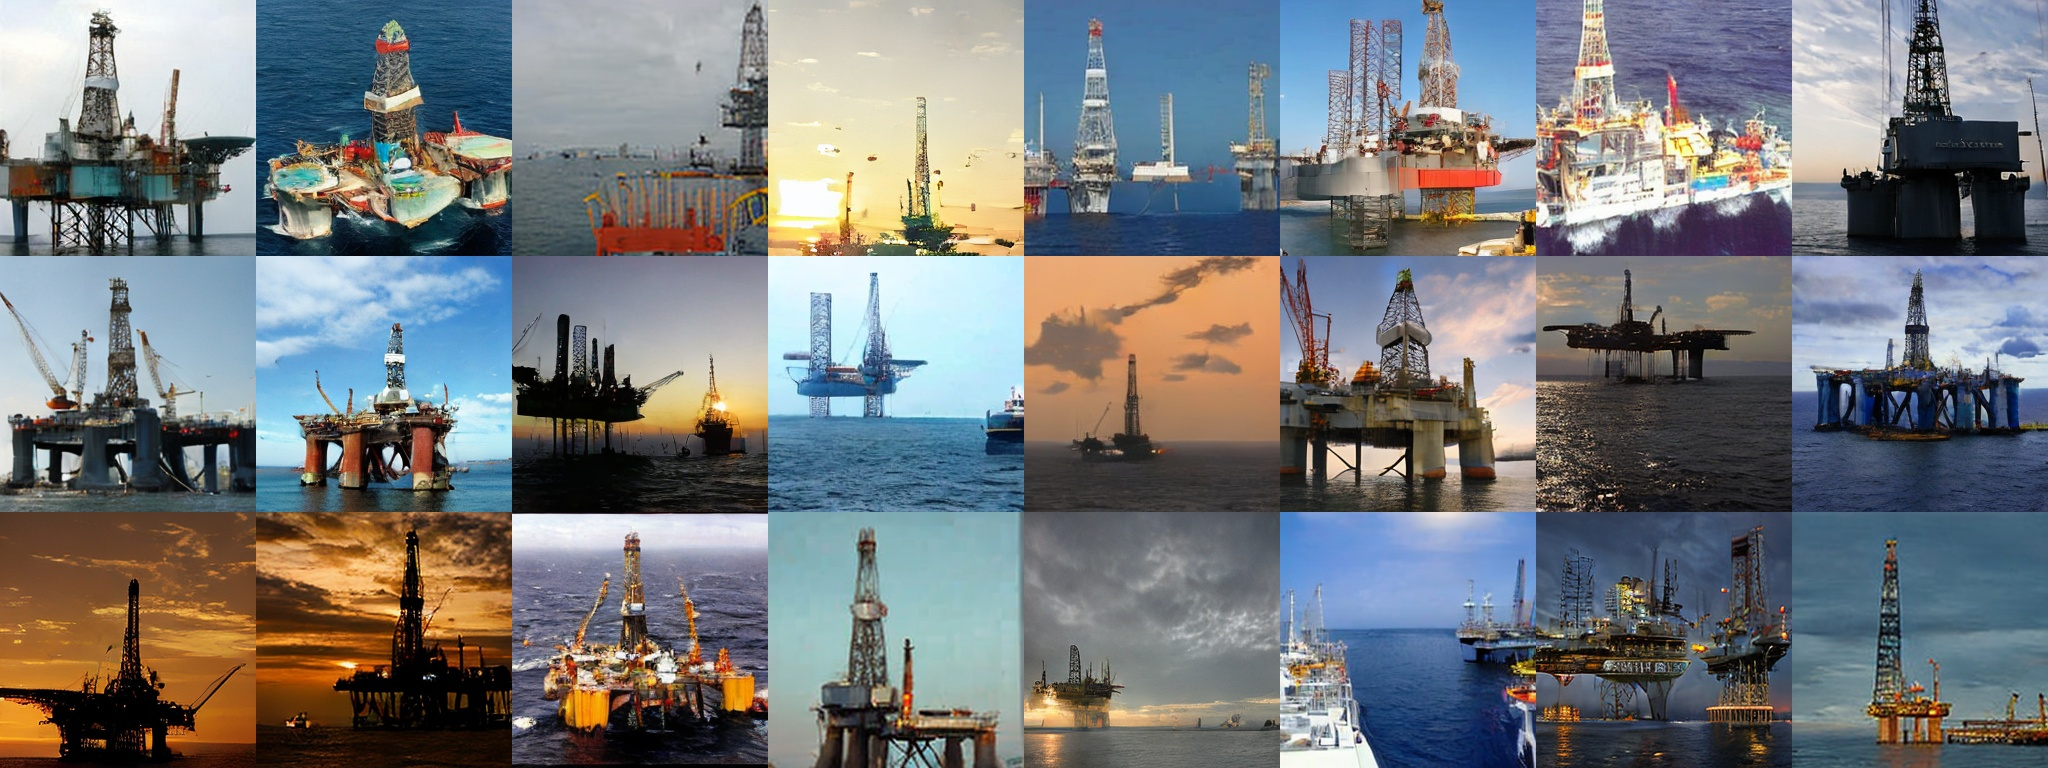
\includegraphics[width=\linewidth]{figures/imf_images/540.jpg}
    \end{minipage}\\[-0.2em]
    \centering\small Class 540: Drilling platform\\[0.2em]
    
    % Class 562: Fountain
    \begin{minipage}[b]{0.48\textwidth}
        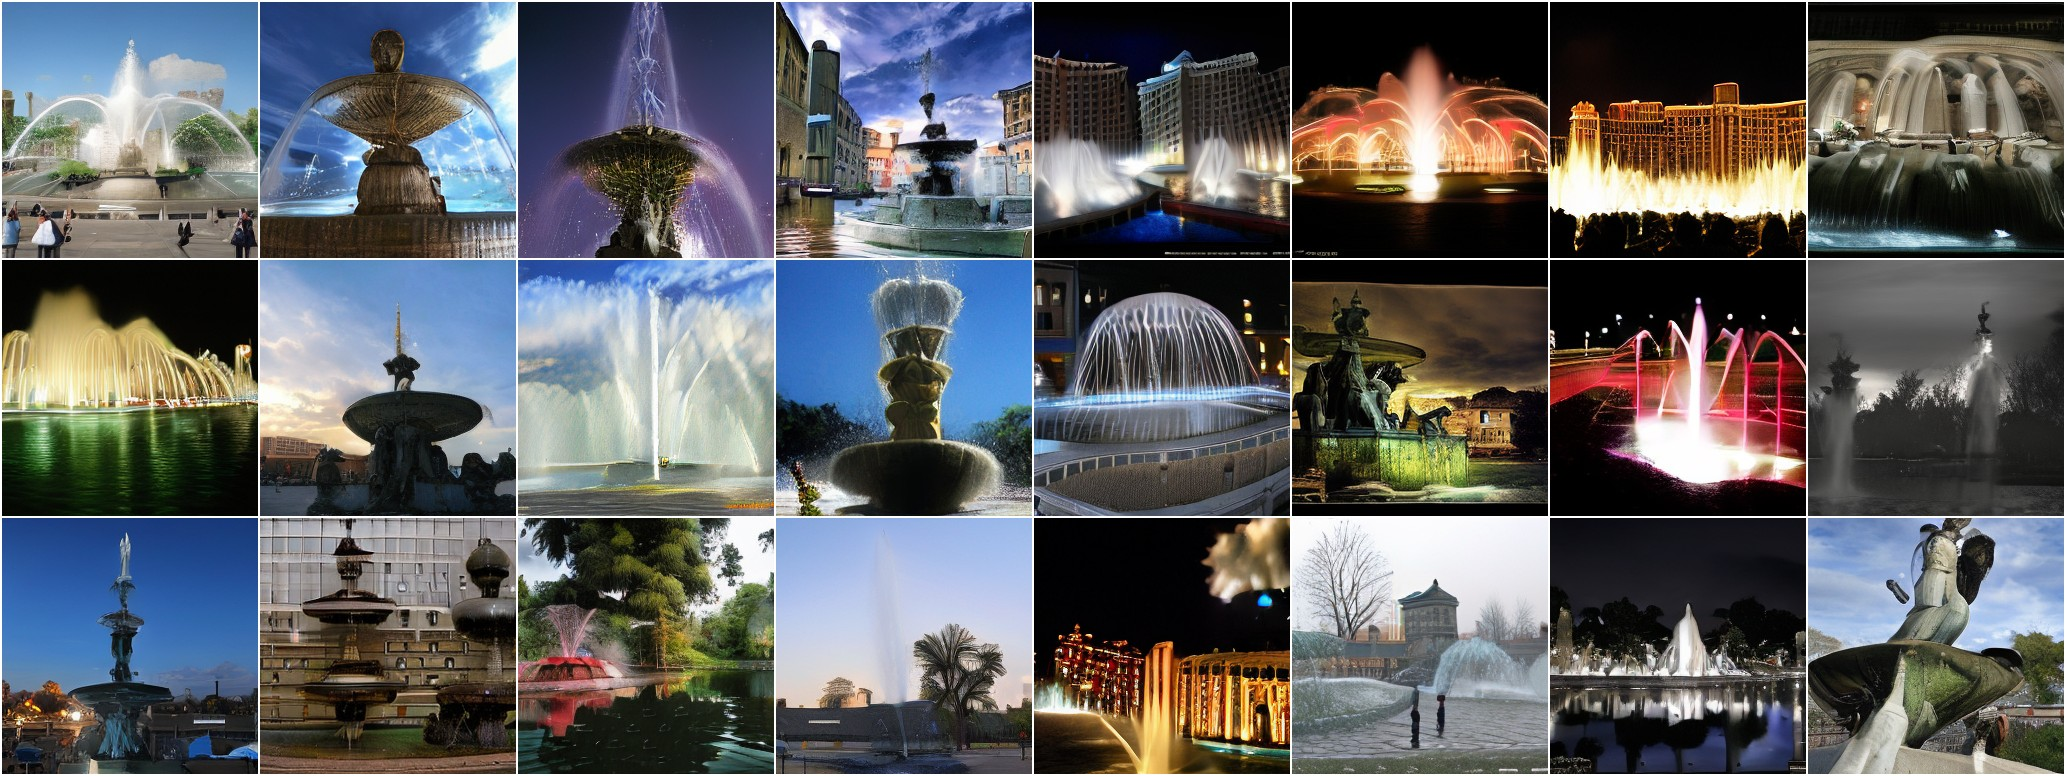
\includegraphics[width=\linewidth]{figures/imf_images/drift/classrank0106_class562_fountain_score5.06.jpg}
    \end{minipage}\hfill
    \begin{minipage}[b]{0.48\textwidth}
        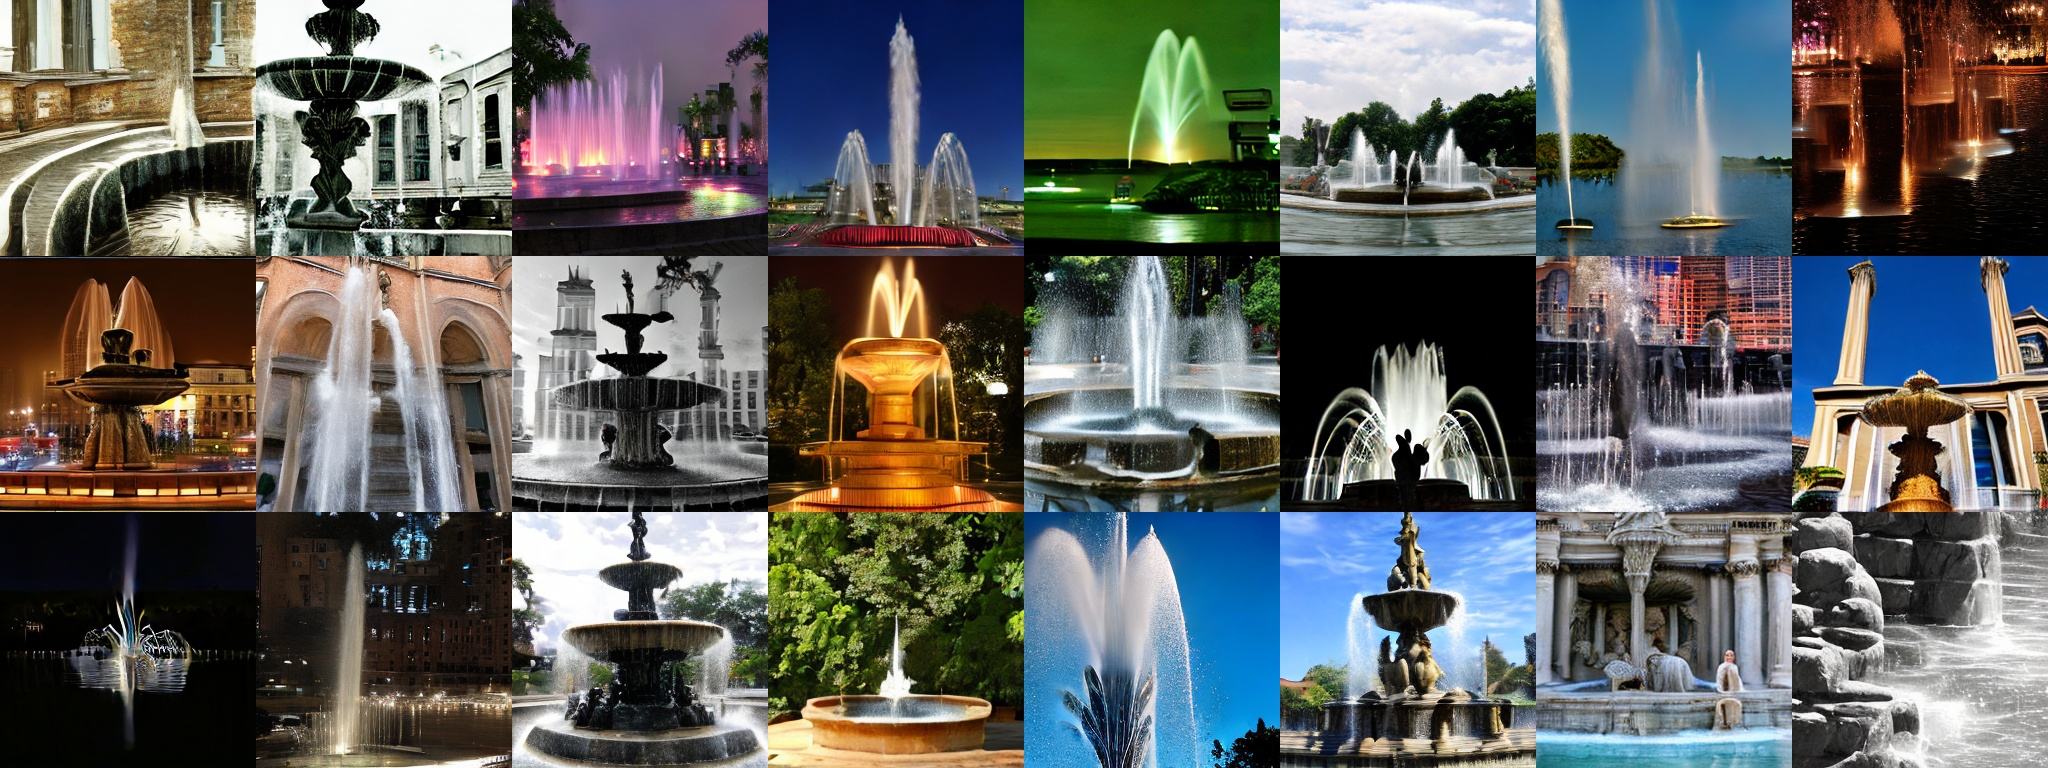
\includegraphics[width=\linewidth]{figures/imf_images/562.jpg}
    \end{minipage}\\[-0.2em]
    \centering\small Class 562: Fountain\\[0.2em]
    
    % Class 649: Megalith
    \begin{minipage}[b]{0.48\textwidth}
        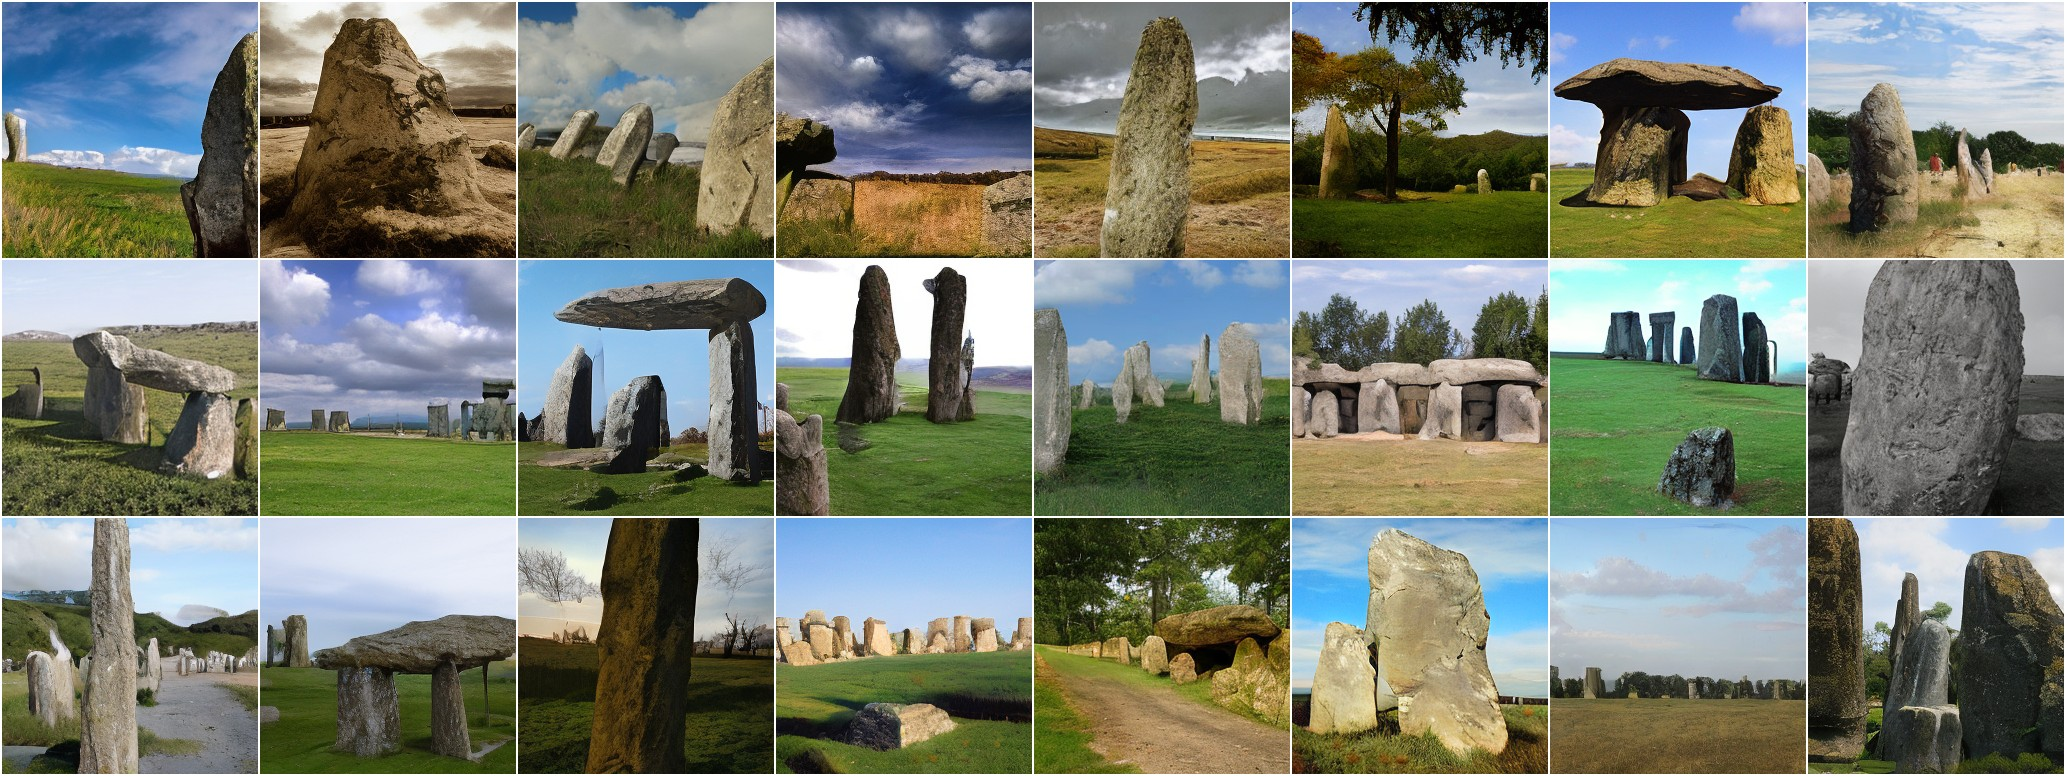
\includegraphics[width=\linewidth]{figures/imf_images/drift/classrank0070_class649_megalith_score5.12.jpg}
    \end{minipage}\hfill
    \begin{minipage}[b]{0.48\textwidth}
        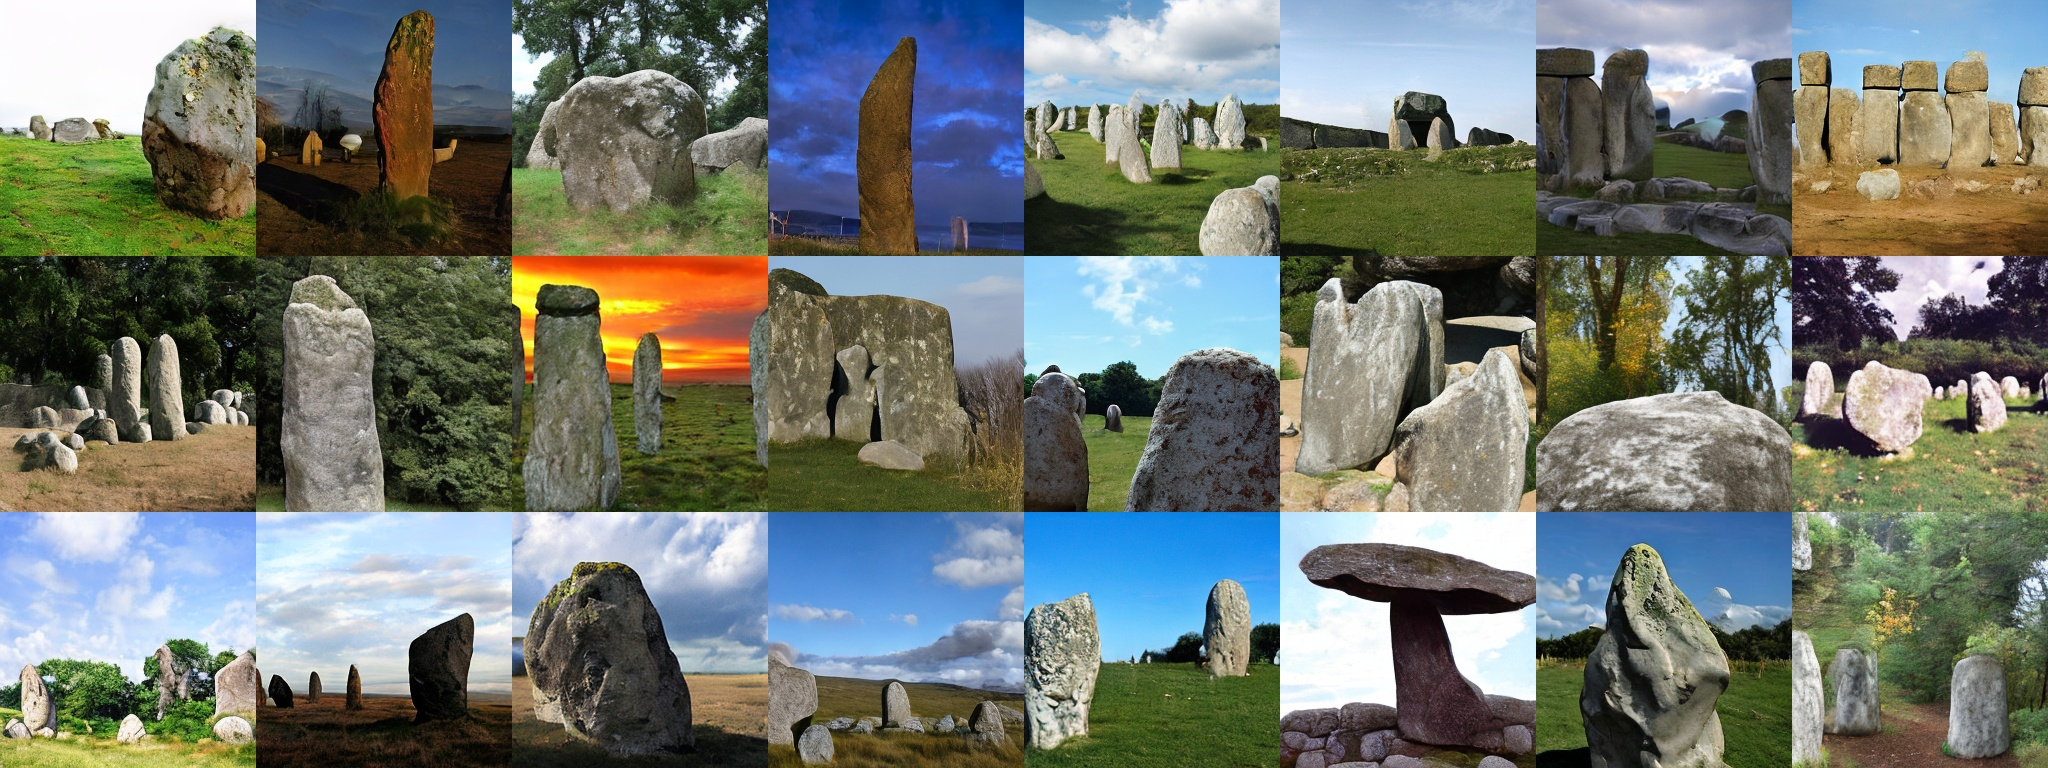
\includegraphics[width=\linewidth]{figures/imf_images/649.jpg}
    \end{minipage}\\[-0.2em]
    \centering\small Class 649: Megalith
    
    \caption{\textbf{Side-by-side comparison with improved MeanFlow (iMF)~\cite{geng2025improved} (page 3/5).} Uncurated samples from our method (left) and iMF (right) on \textbf{all} ImageNet classes visualized in the iMF paper. Both methods generate images with a single neural function evaluation (1-NFE). The iMF visualizations use CFG $\omega{=}6.0$ and interval $[t_\text{min}, t_\text{max}]{=}[0.2, 0.8]$, achieving FID 3.92 and IS 348.2 (DiT-XL/2). For fair comparison, we set the CFG scale to match the IS of iMF visualizations, which leads to FID 3.01 and IS 354.4 (at CFG=1.5) for our method (DiT-L/2).}
    \label{fig:comparison_imf_3}
\end{figure*}

\begin{figure*}[p]
    \centering
    % Header
    \begin{minipage}{0.48\textwidth}
        \centering{ours}
    \end{minipage}\hfill
    \begin{minipage}{0.48\textwidth}
        \centering{improved MeanFlow (iMF)}
    \end{minipage}\\[0.2em]
    
    % Class 698: Palace
    \begin{minipage}[b]{0.48\textwidth}
        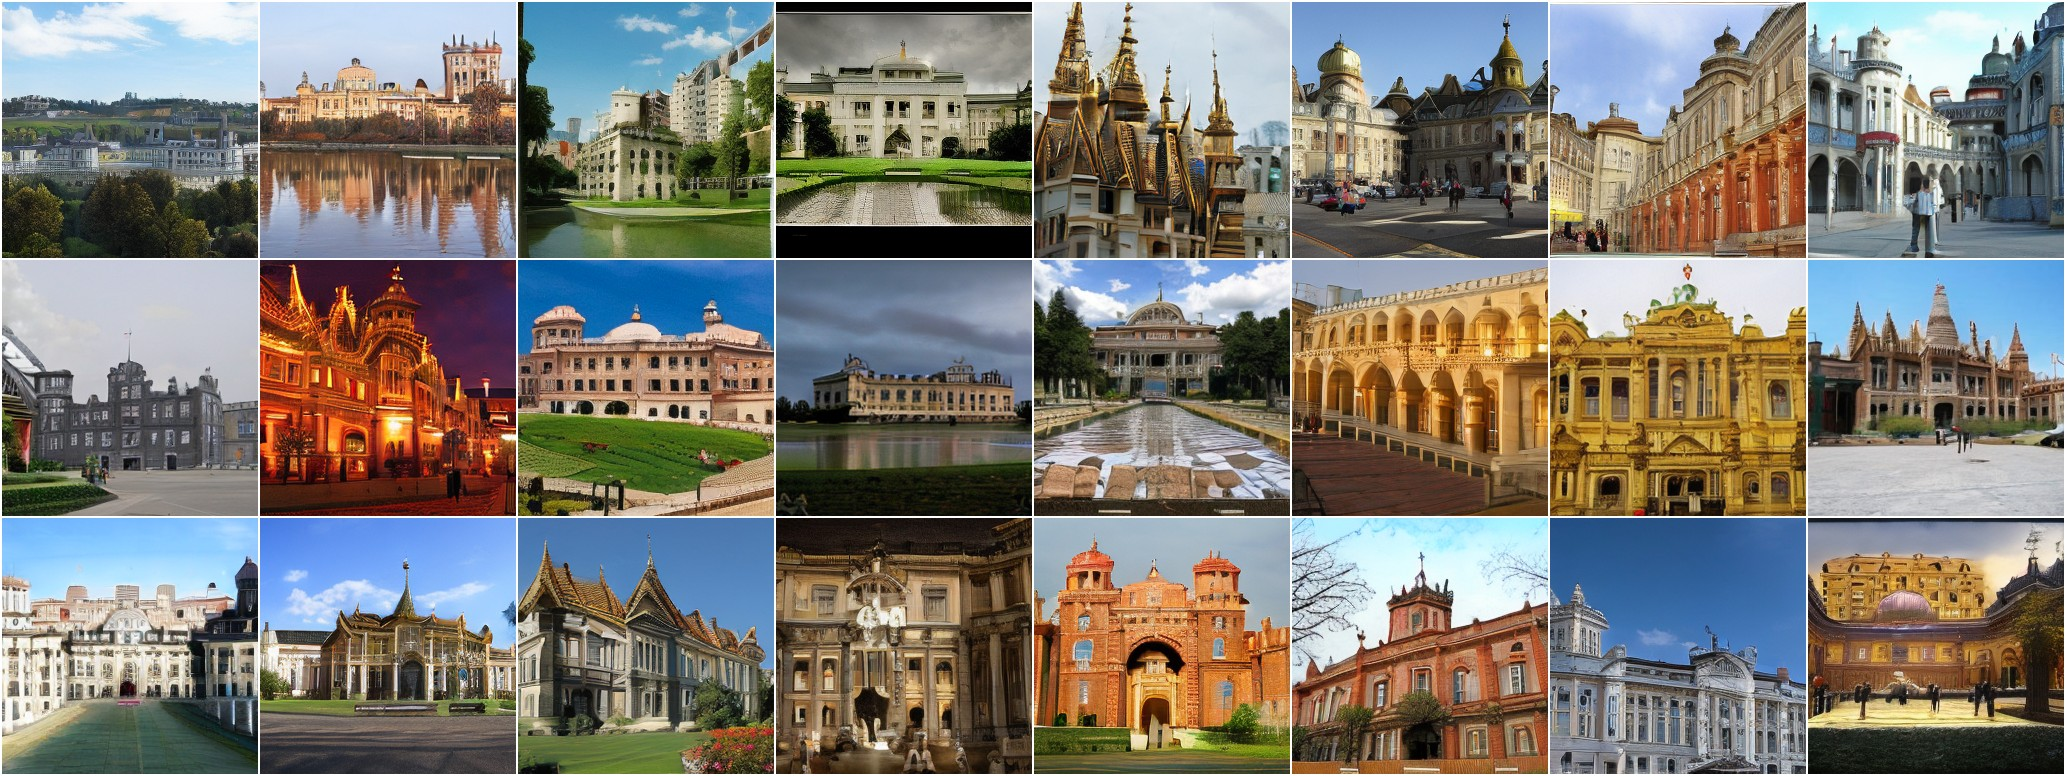
\includegraphics[width=\linewidth]{figures/imf_images/drift/classrank0105_class698_palace_score5.06.jpg}
    \end{minipage}\hfill
    \begin{minipage}[b]{0.48\textwidth}
        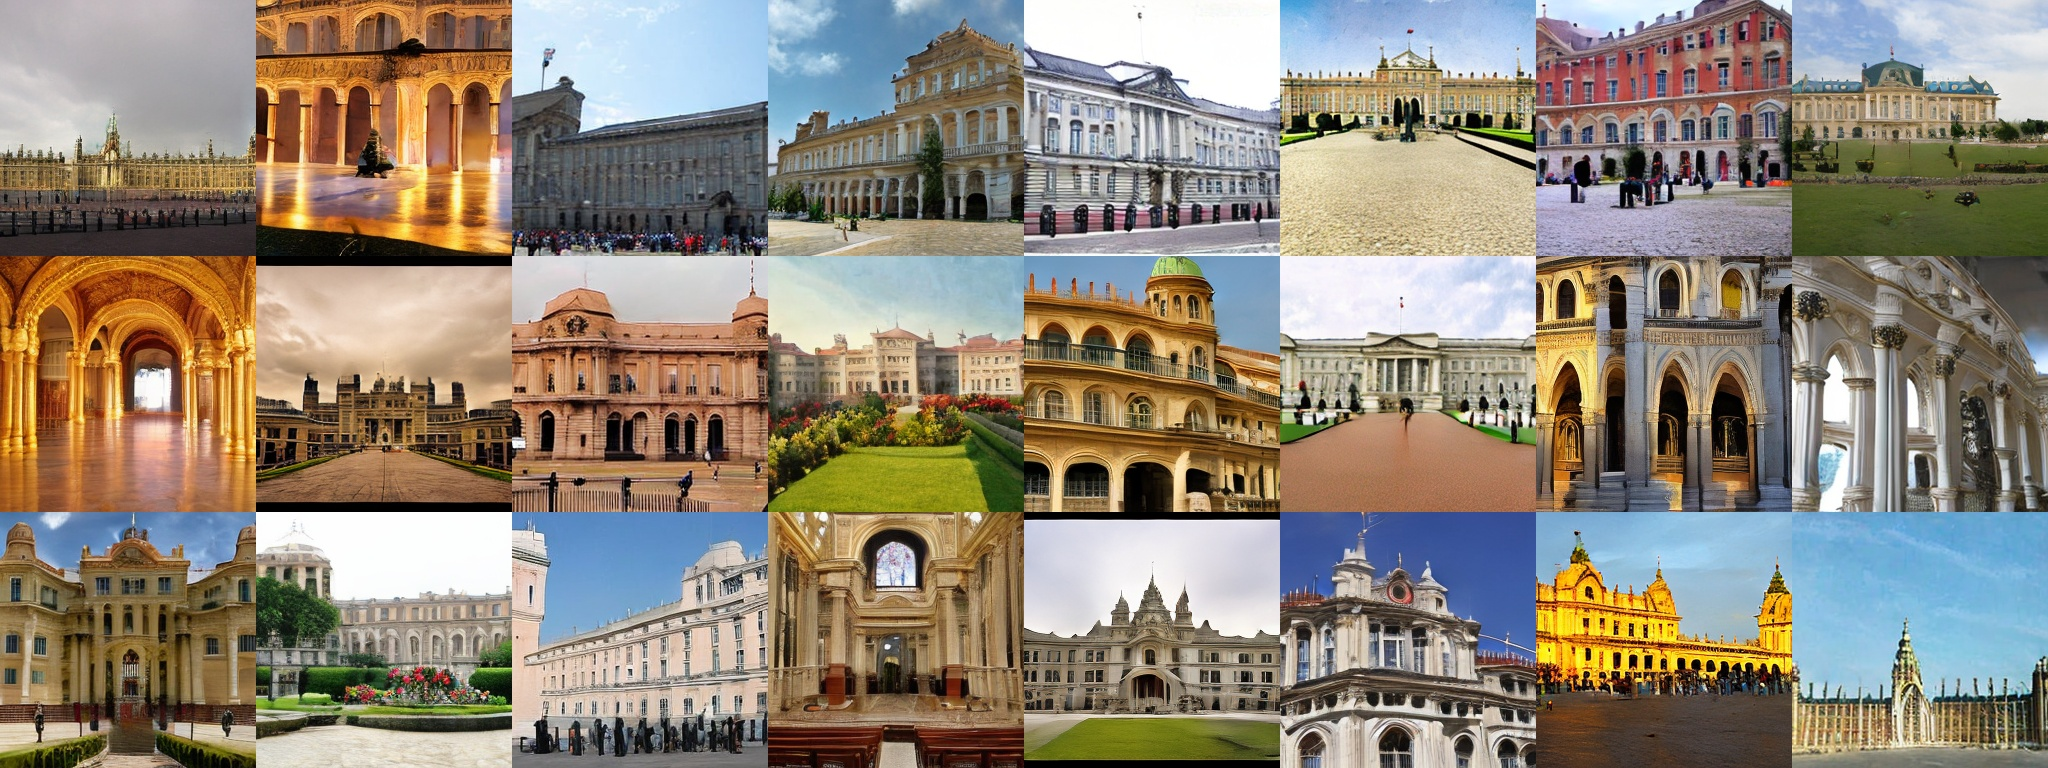
\includegraphics[width=\linewidth]{figures/imf_images/698.jpg}
    \end{minipage}\\[-0.2em]
    \centering\small Class 698: Palace\\[0.2em]
    
    % Class 738: Pot
    \begin{minipage}[b]{0.48\textwidth}
        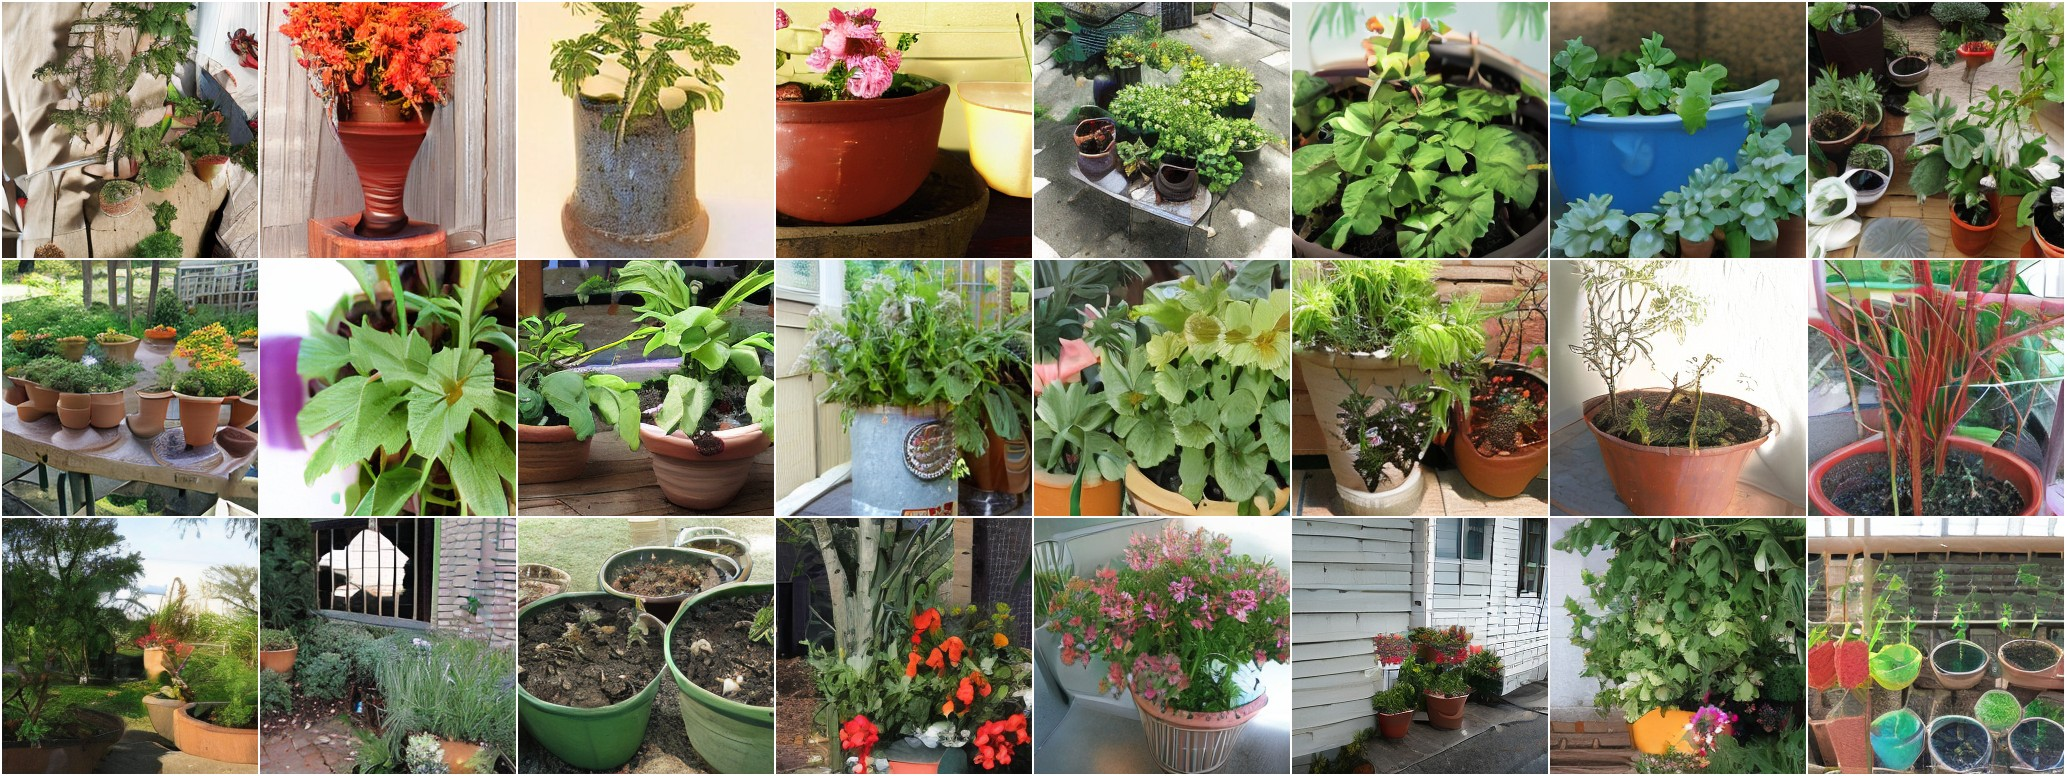
\includegraphics[width=\linewidth]{figures/imf_images/drift/classrank0643_class738_pot_score4.55.jpg}
    \end{minipage}\hfill
    \begin{minipage}[b]{0.48\textwidth}
        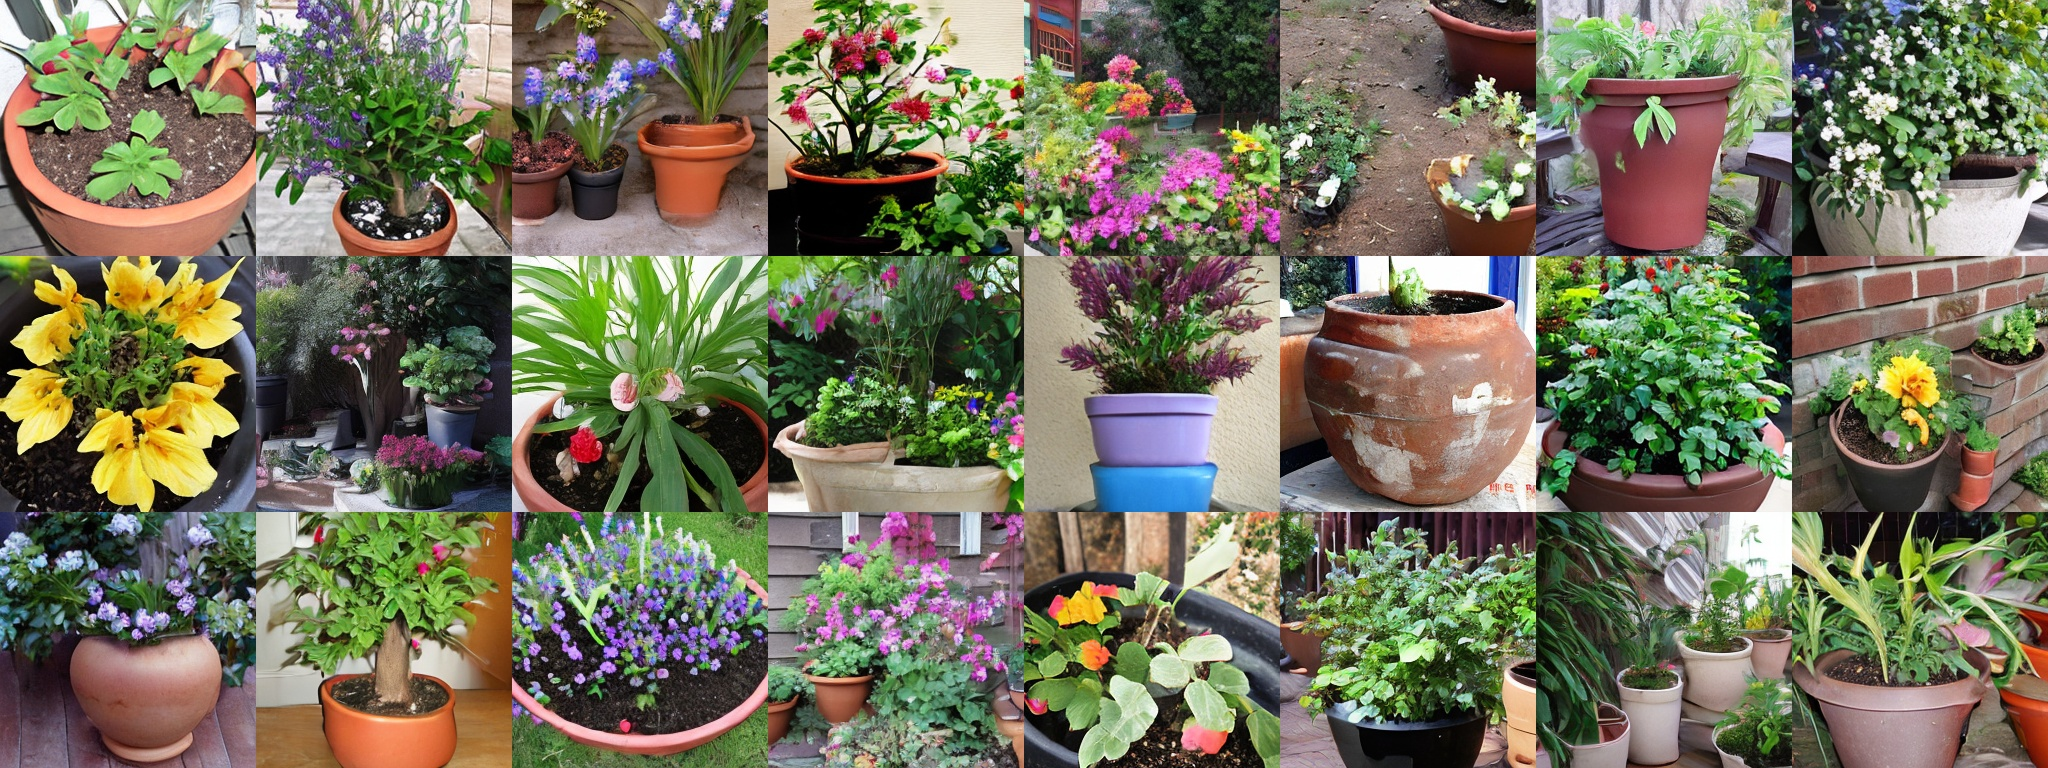
\includegraphics[width=\linewidth]{figures/imf_images/738.jpg}
    \end{minipage}\\[-0.2em]
    \centering\small Class 738: Pot\\[0.2em]
    
    % Class 963: Pizza
    \begin{minipage}[b]{0.48\textwidth}
        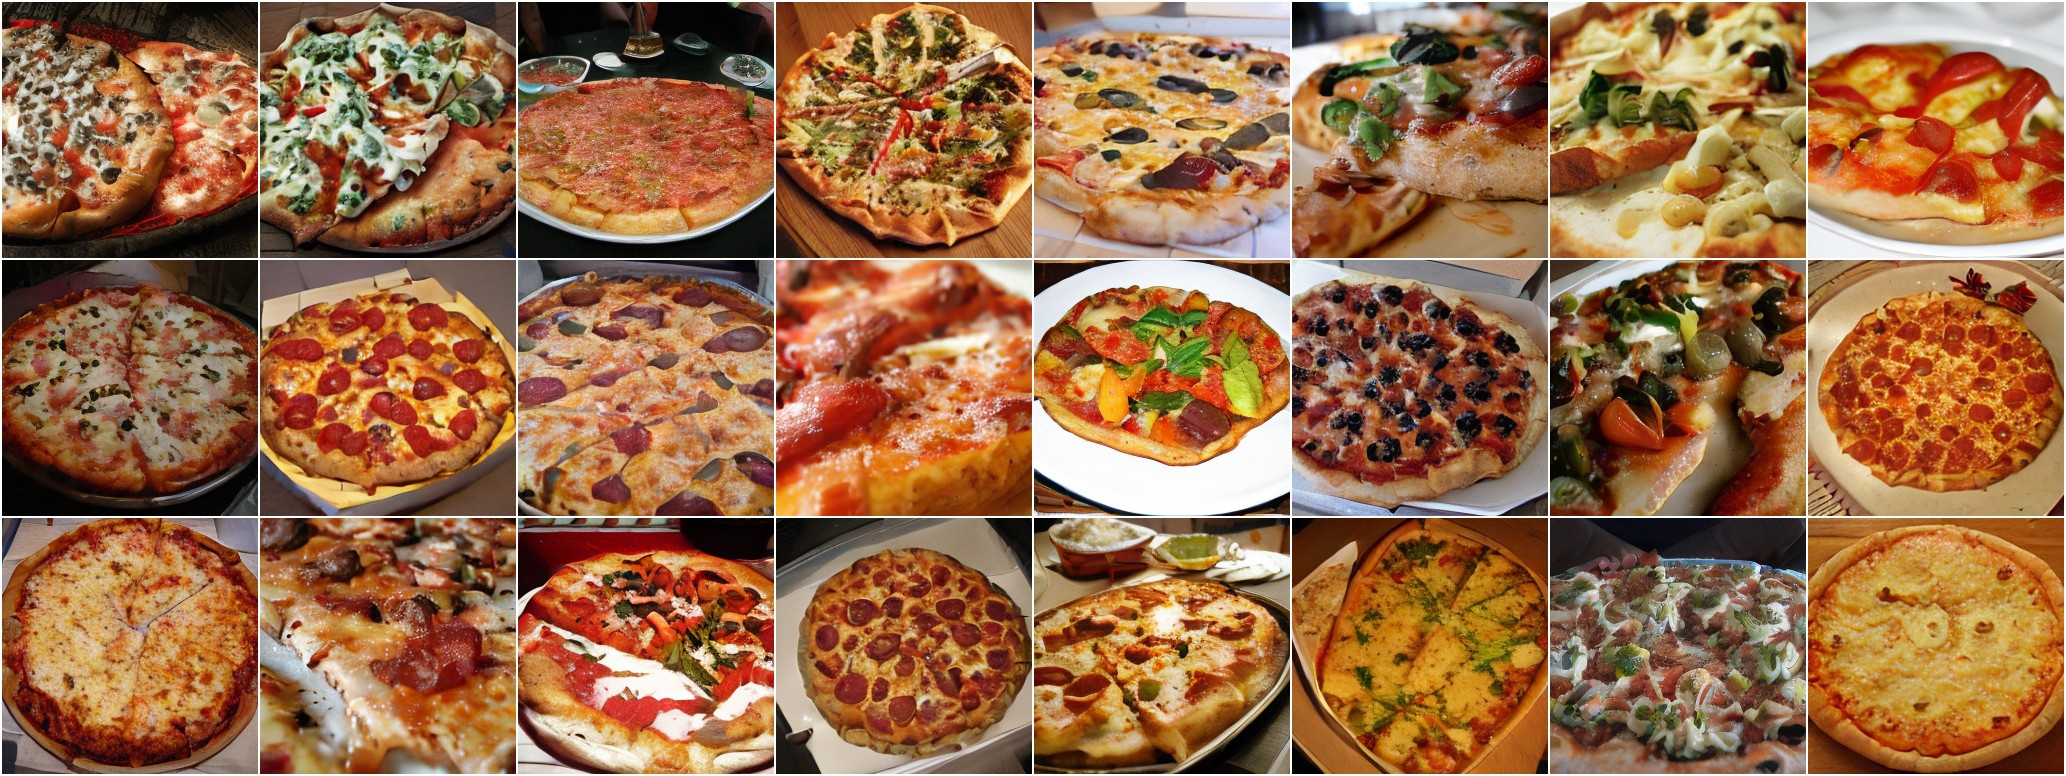
\includegraphics[width=\linewidth]{figures/imf_images/drift/classrank0306_class963_pizza_score4.80.jpg}
    \end{minipage}\hfill
    \begin{minipage}[b]{0.48\textwidth}
        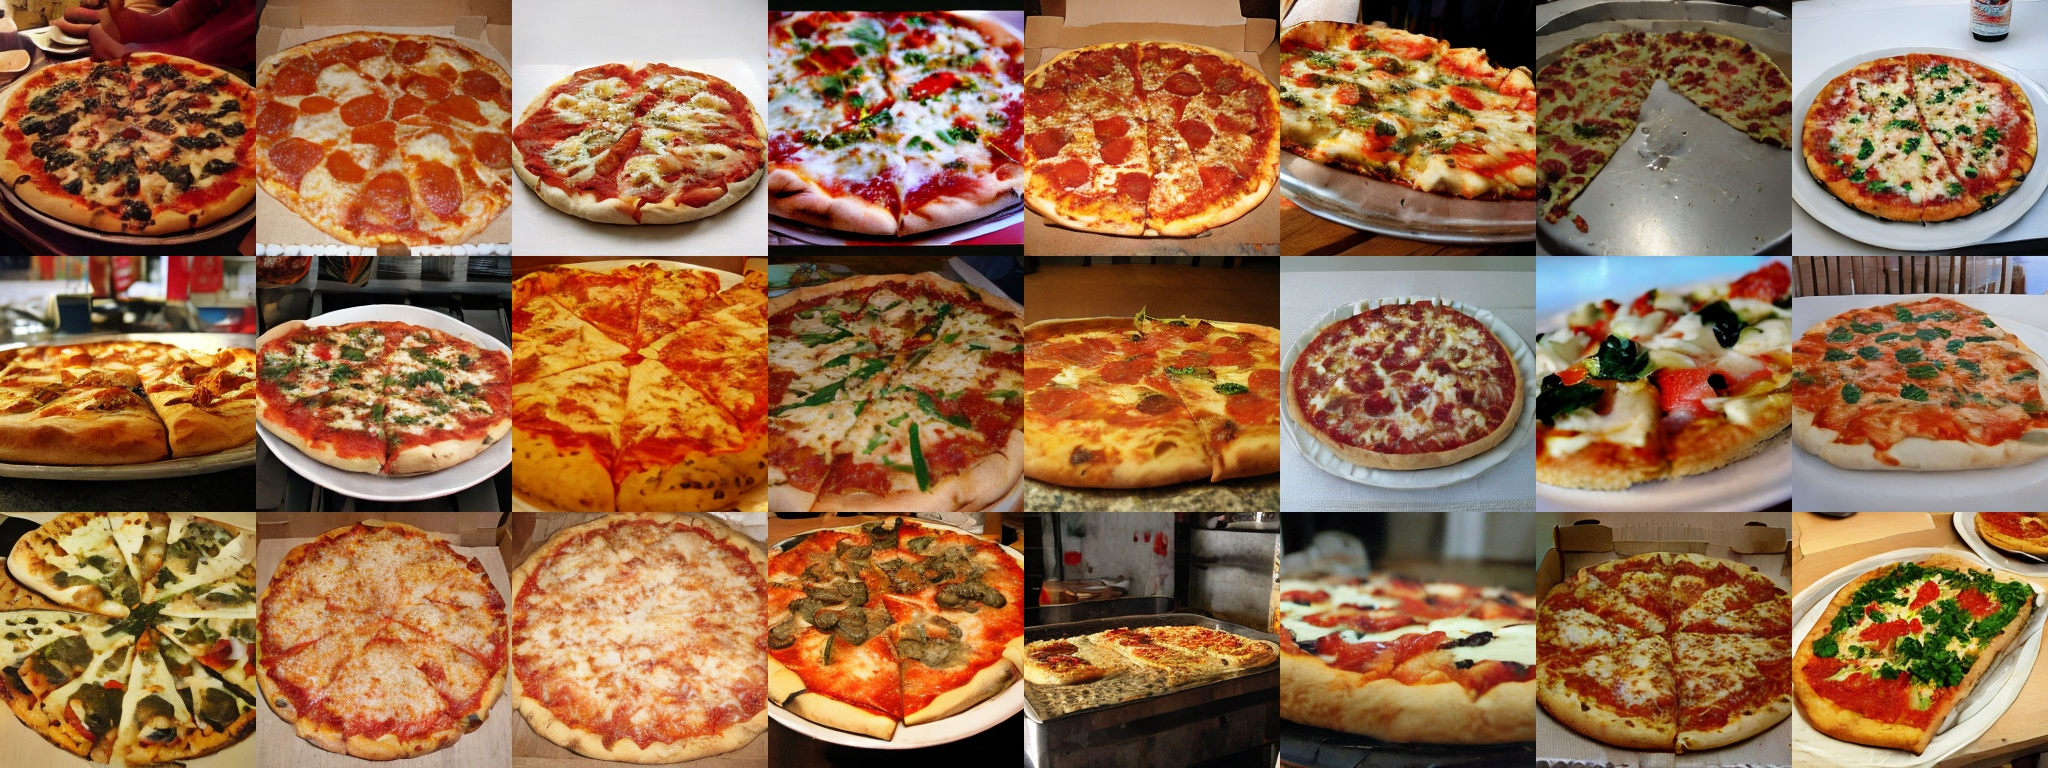
\includegraphics[width=\linewidth]{figures/imf_images/963.jpg}
    \end{minipage}\\[-0.2em]
    \centering\small Class 963: Pizza\\[0.2em]
    
    % Class 970: Alp
    \begin{minipage}[b]{0.48\textwidth}
        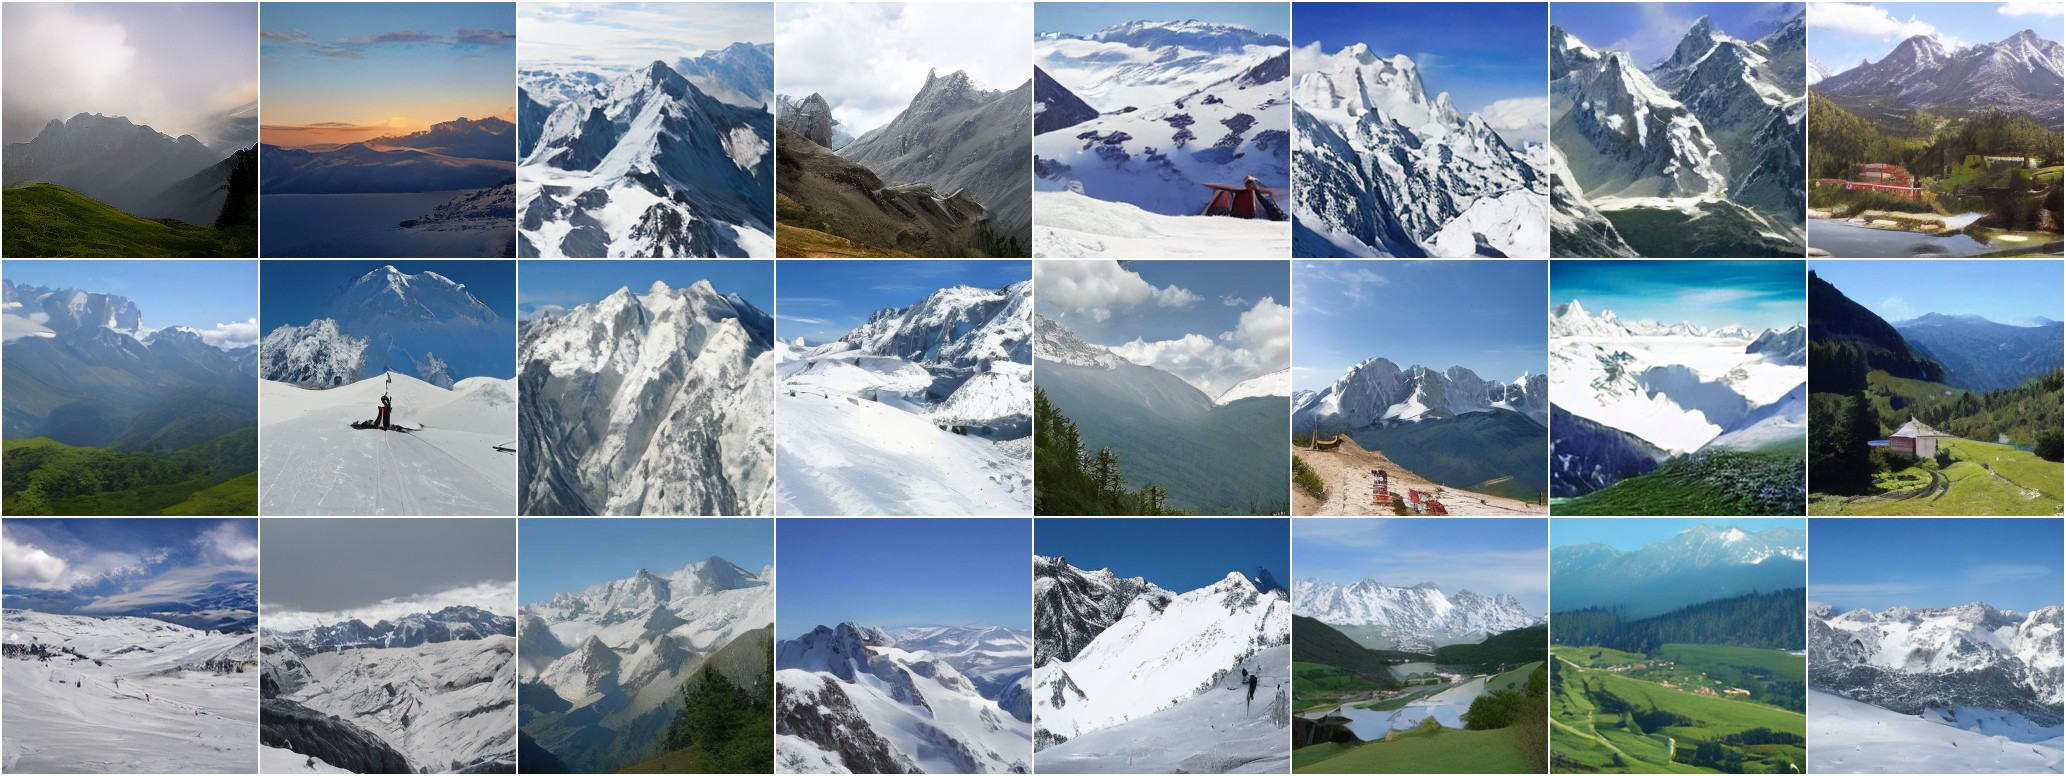
\includegraphics[width=\linewidth]{figures/imf_images/drift/classrank0027_class970_alp_score5.26.jpg}
    \end{minipage}\hfill
    \begin{minipage}[b]{0.48\textwidth}
        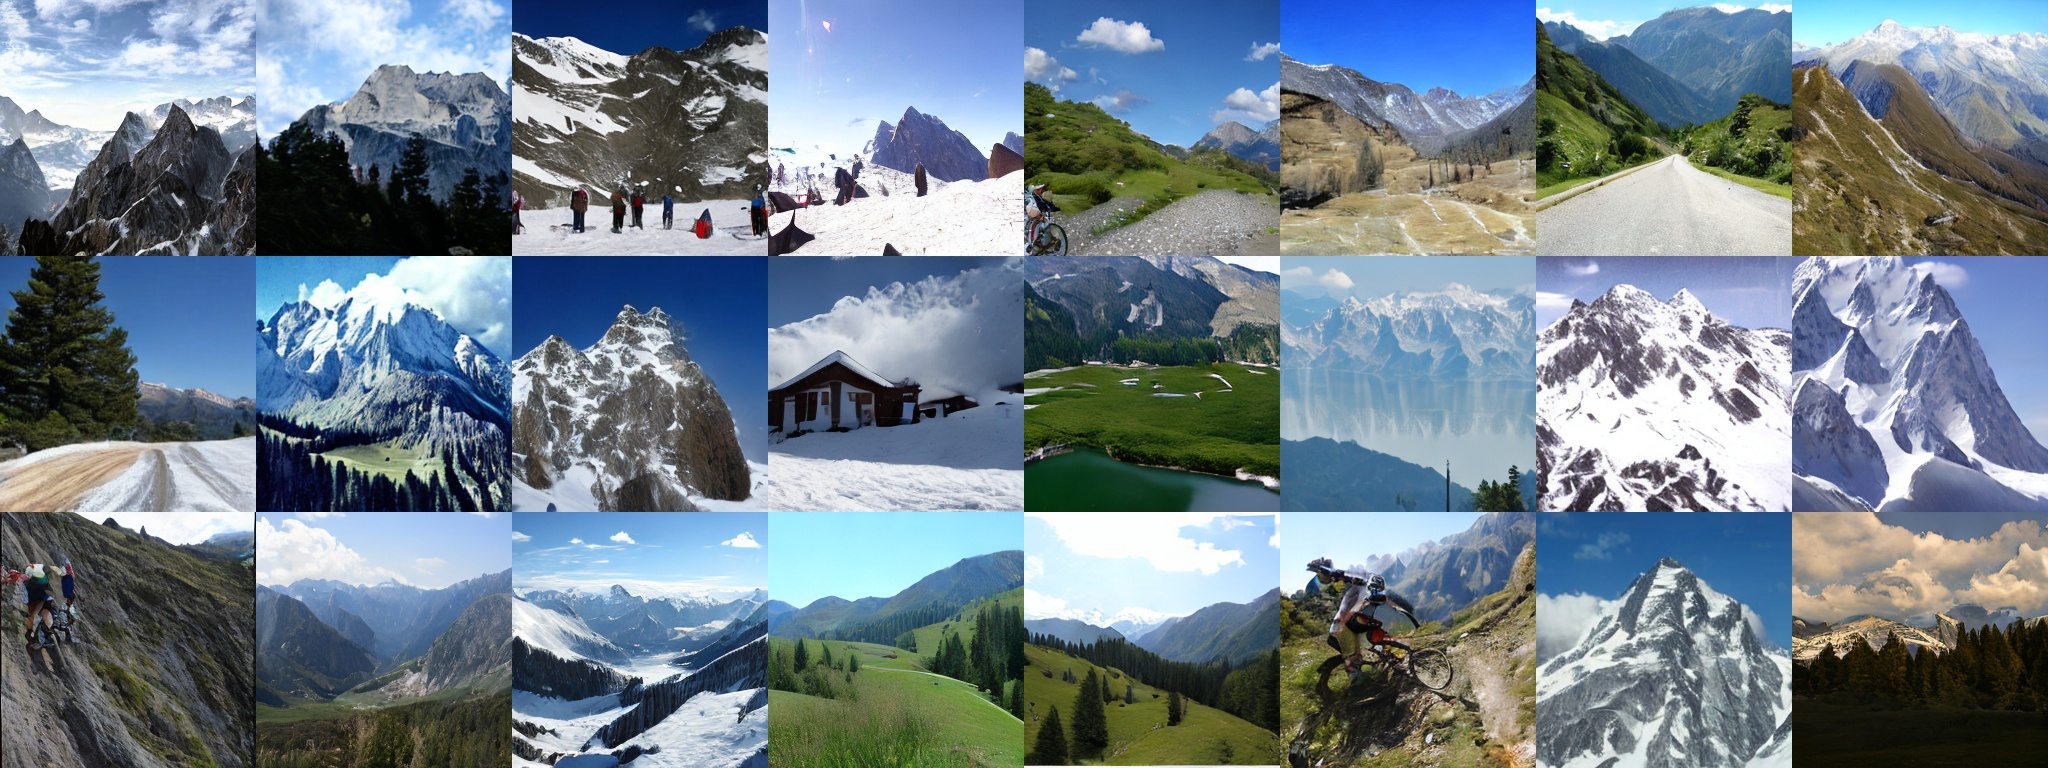
\includegraphics[width=\linewidth]{figures/imf_images/970.jpg}
    \end{minipage}\\[-0.2em]
    \centering\small Class 970: Alp\\[0.2em]
    
    % Class 973: Coral reef
    \begin{minipage}[b]{0.48\textwidth}
        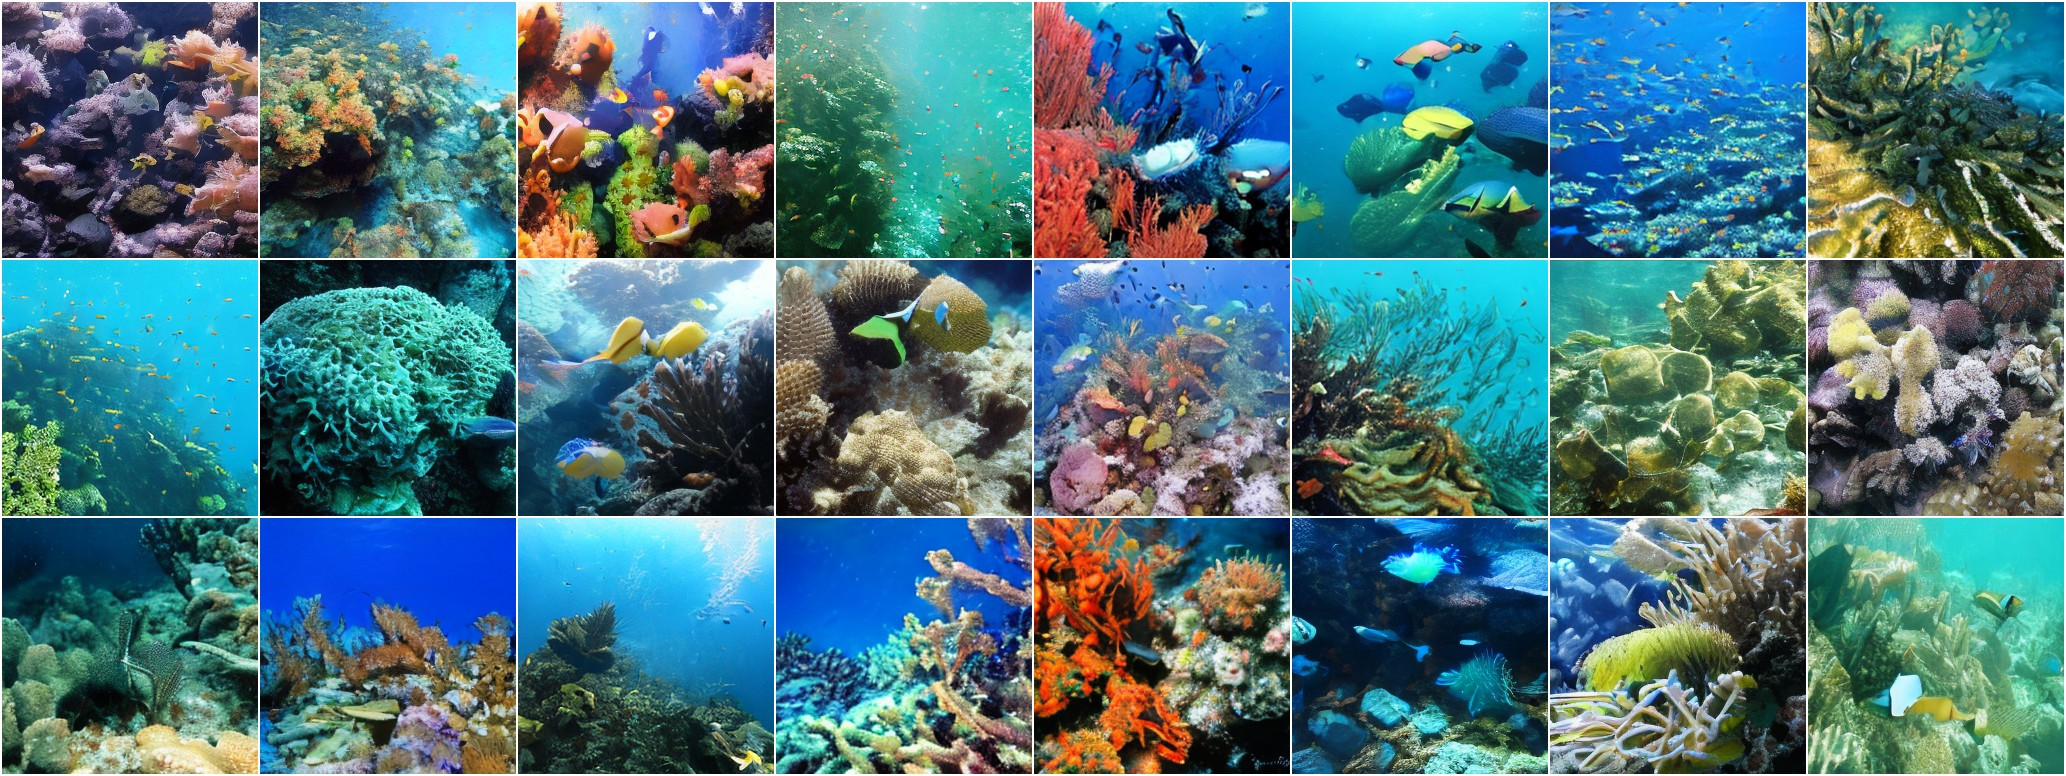
\includegraphics[width=\linewidth]{figures/imf_images/drift/classrank0180_class973_coral_reef_score4.95.jpg}
    \end{minipage}\hfill
    \begin{minipage}[b]{0.48\textwidth}
        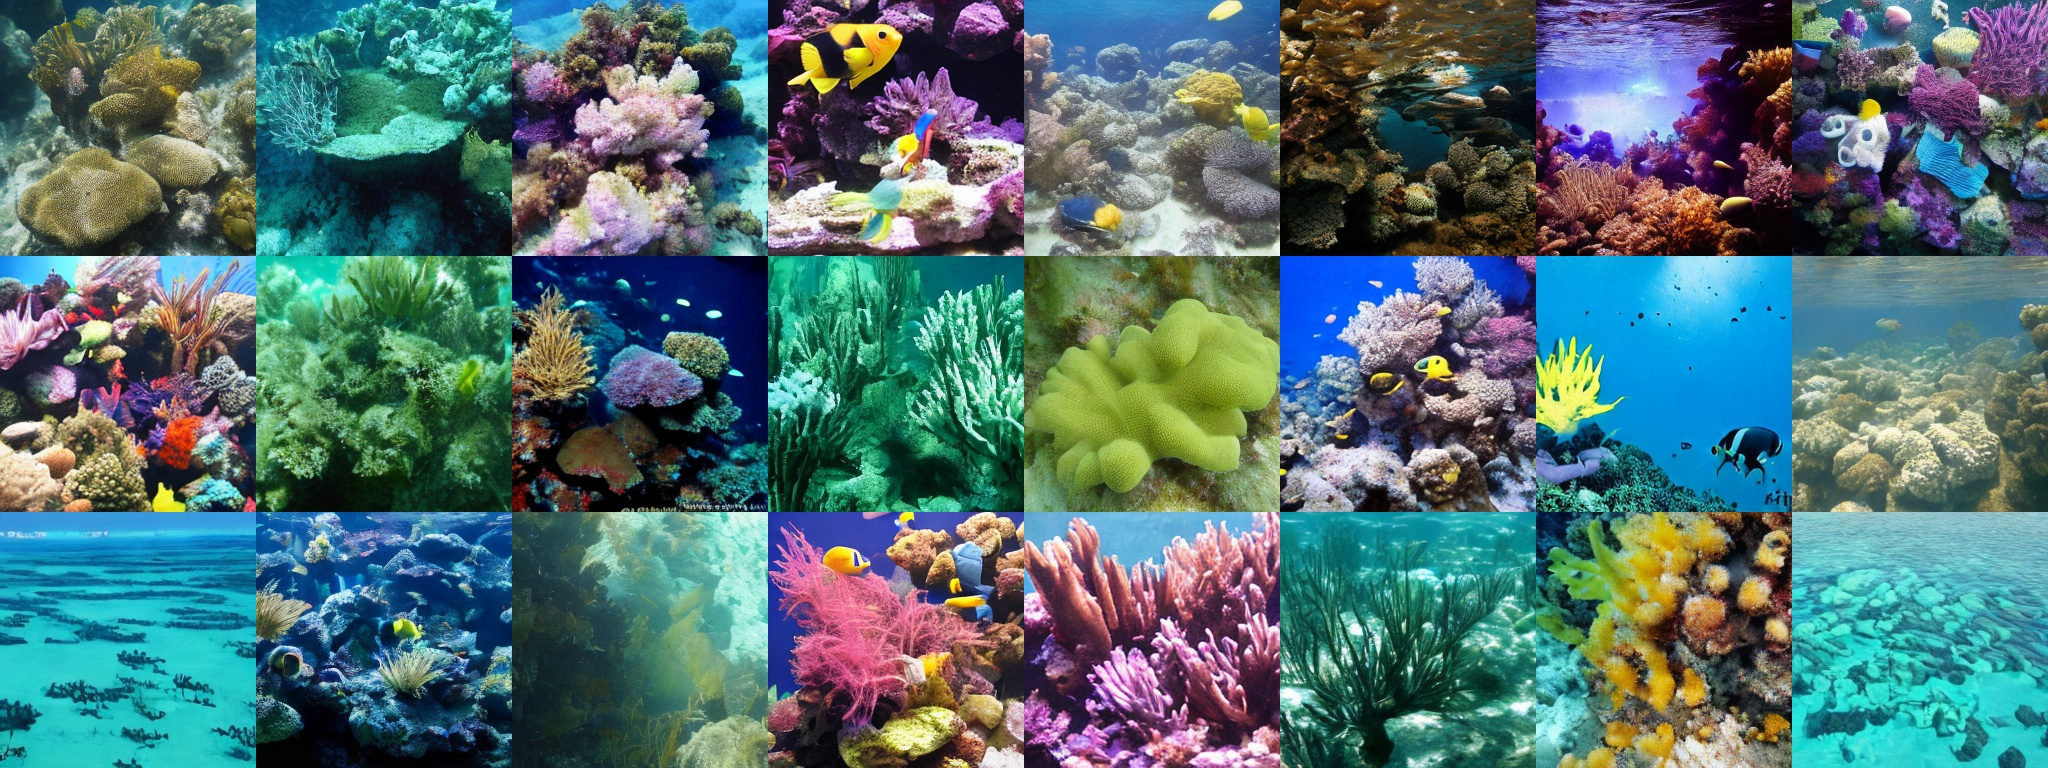
\includegraphics[width=\linewidth]{figures/imf_images/973.jpg}
    \end{minipage}\\[-0.2em]
    \centering\small Class 973: Coral reef
    
    \caption{\textbf{Side-by-side comparison with improved MeanFlow (iMF)~\cite{geng2025improved} (page 4/5).} Uncurated samples from our method (left) and iMF (right) on \textbf{all} ImageNet classes visualized in the iMF paper. Both methods generate images with a single neural function evaluation (1-NFE). The iMF visualizations use CFG $\omega{=}6.0$ and interval $[t_\text{min}, t_\text{max}]{=}[0.2, 0.8]$, achieving FID 3.92 and IS 348.2 (DiT-XL/2). For fair comparison, we set the CFG scale to match the IS of iMF visualizations, which leads to FID 3.01 and IS 354.4 (at CFG=1.5) for our method (DiT-L/2).}
    \label{fig:comparison_imf_4}
\end{figure*}

\begin{figure*}[p]
    \centering
    % Header
    \begin{minipage}{0.48\textwidth}
        \centering{ours}
    \end{minipage}\hfill
    \begin{minipage}{0.48\textwidth}
        \centering{improved MeanFlow (iMF)}
    \end{minipage}\\[0.2em]
    
    % Class 975: Lakeside
    \begin{minipage}[b]{0.48\textwidth}
        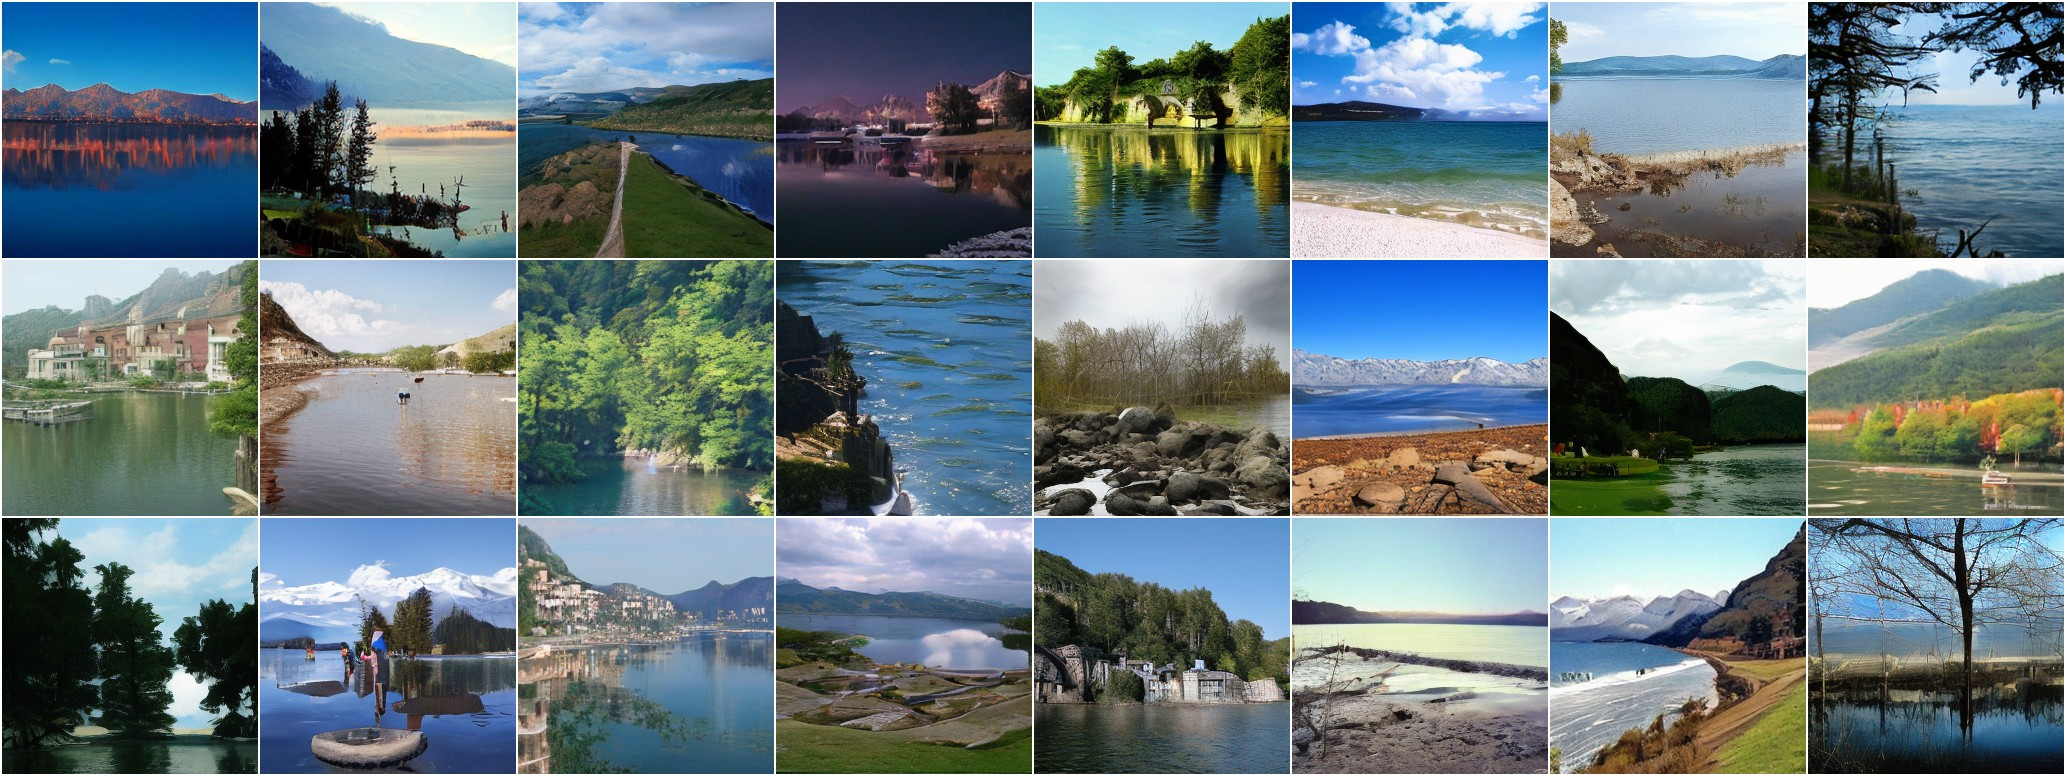
\includegraphics[width=\linewidth]{figures/imf_images/drift/classrank0111_class975_lakeside_score5.05.jpg}
    \end{minipage}\hfill
    \begin{minipage}[b]{0.48\textwidth}
        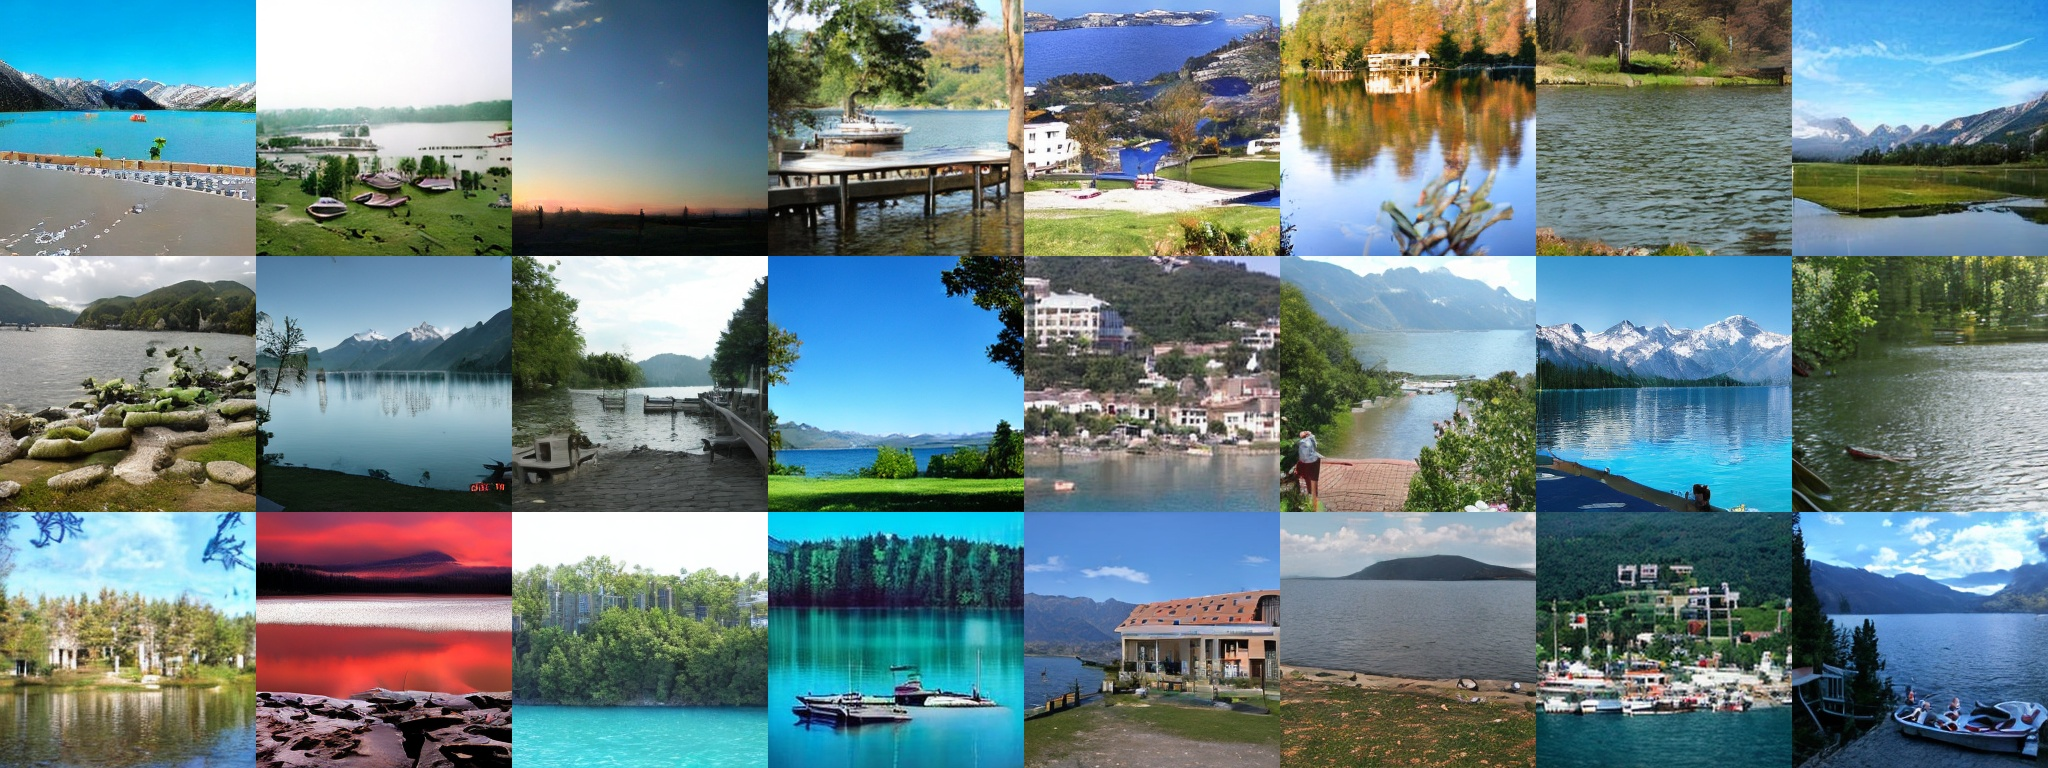
\includegraphics[width=\linewidth]{figures/imf_images/975.jpg}
    \end{minipage}\\[-0.2em]
    \centering\small Class 975: Lakeside\\[0.2em]
    
    % Class 976: Promontory
    \begin{minipage}[b]{0.48\textwidth}
        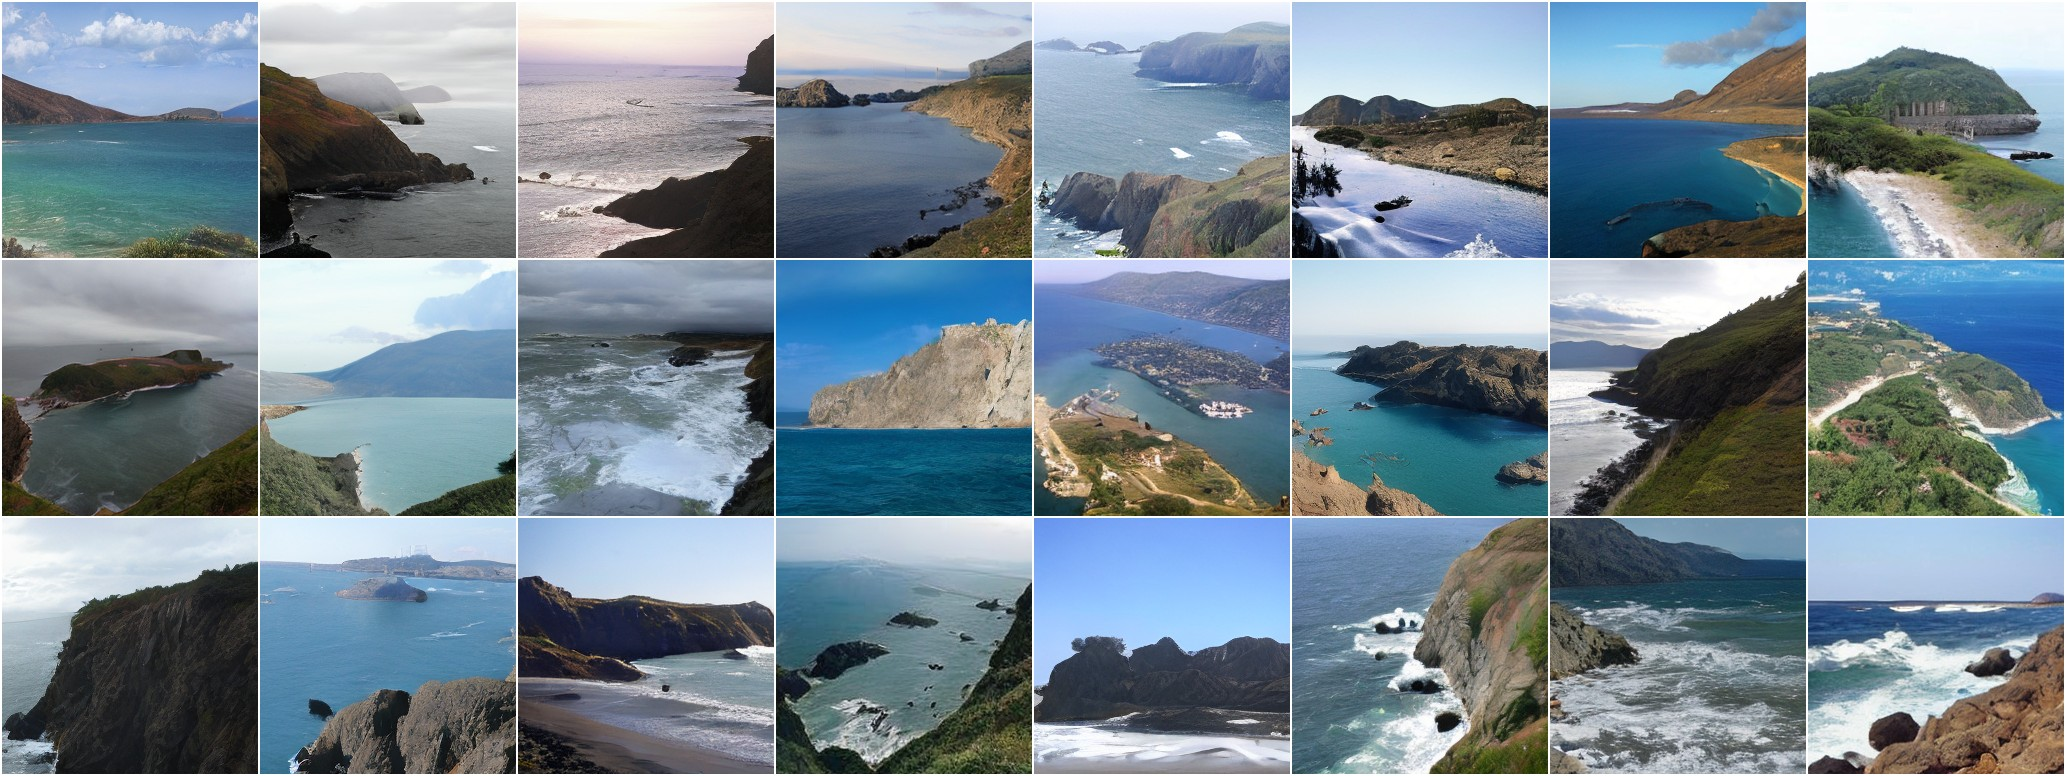
\includegraphics[width=\linewidth]{figures/imf_images/drift/classrank0185_class976_promontory_score4.94.jpg}
    \end{minipage}\hfill
    \begin{minipage}[b]{0.48\textwidth}
        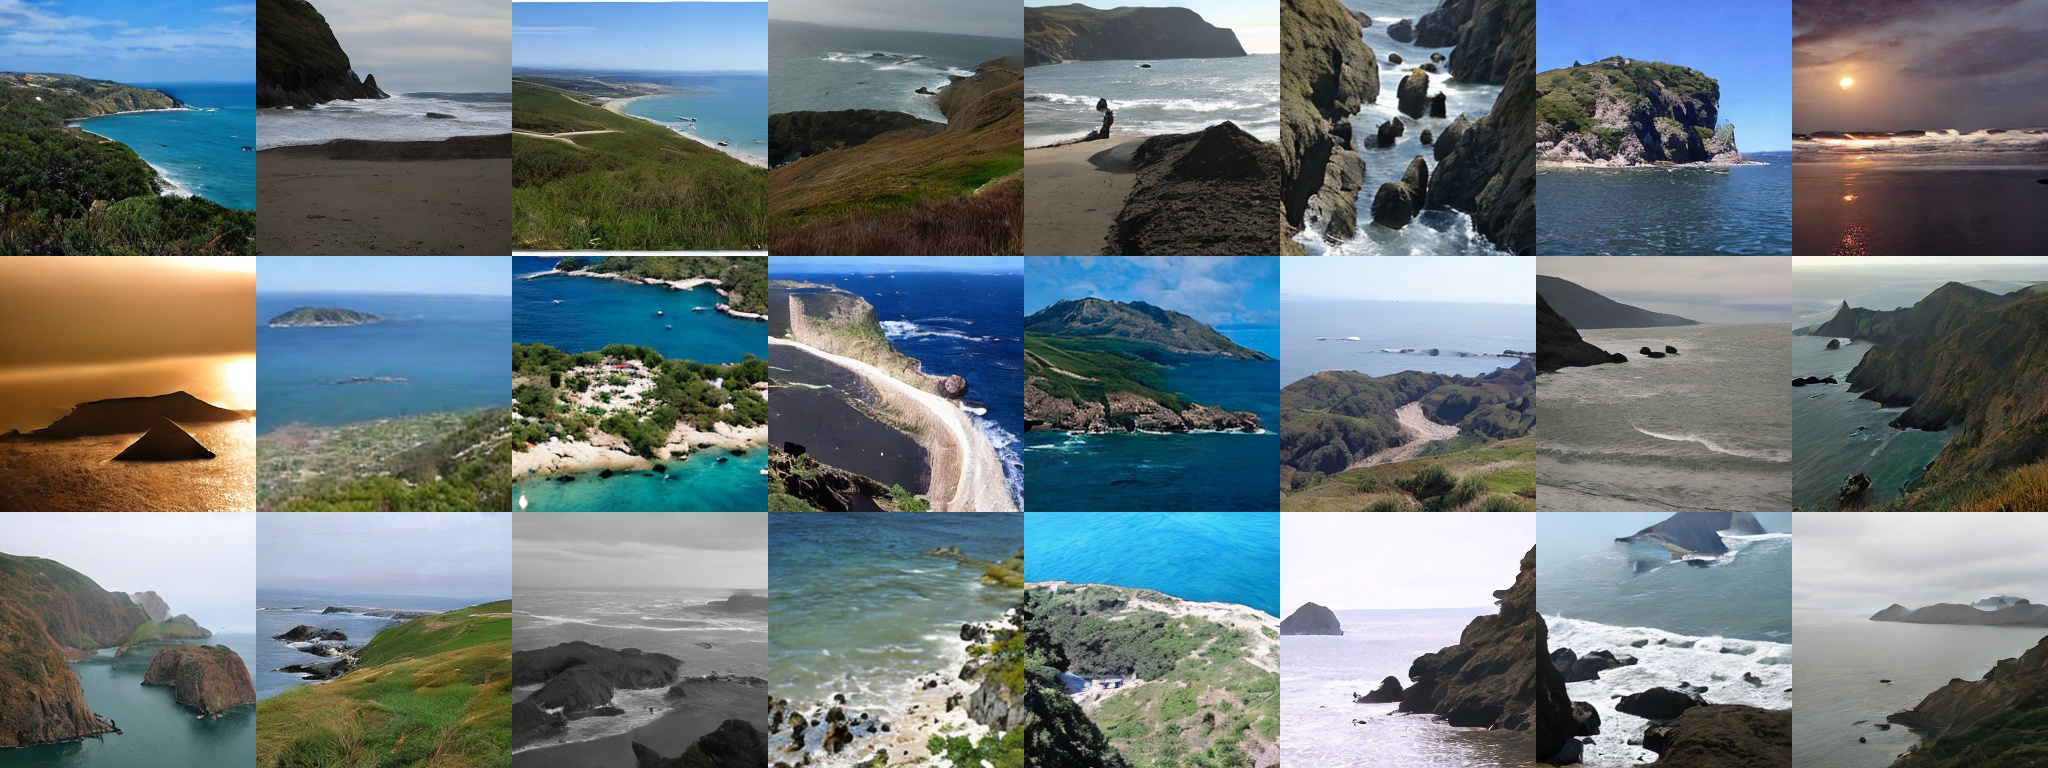
\includegraphics[width=\linewidth]{figures/imf_images/976.jpg}
    \end{minipage}\\[-0.2em]
    \centering\small Class 976: Promontory\\[0.2em]
    
    % Class 985: Daisy
    \begin{minipage}[b]{0.48\textwidth}
        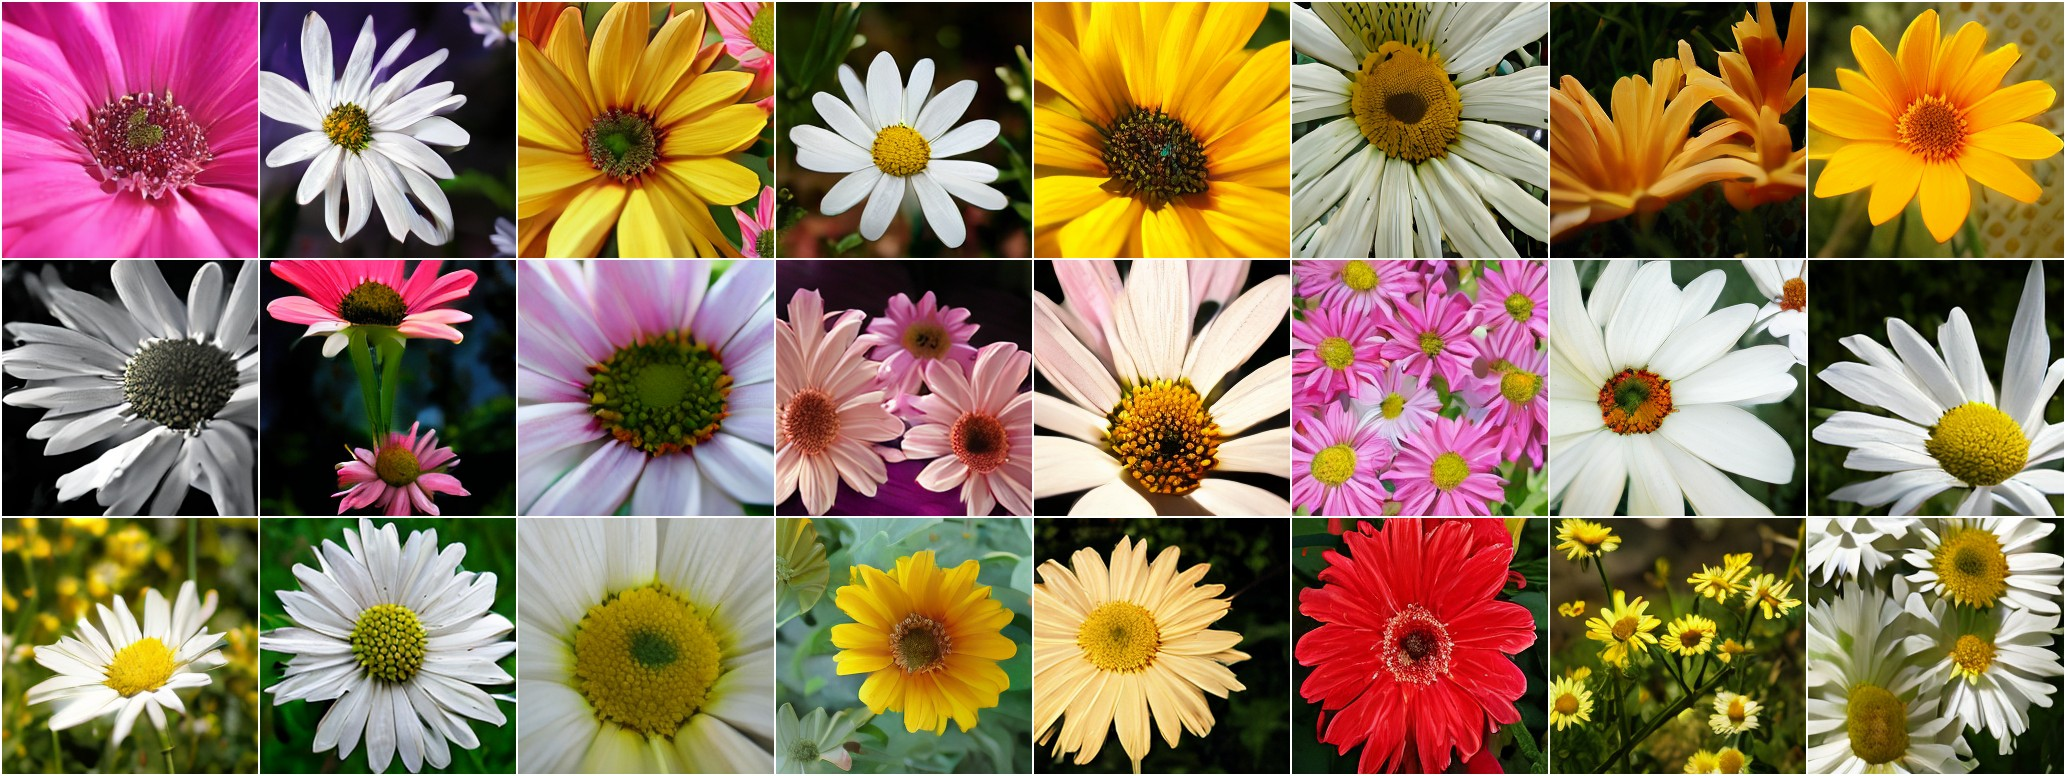
\includegraphics[width=\linewidth]{figures/imf_images/drift/classrank0131_class985_daisy_score5.01.jpg}
    \end{minipage}\hfill
    \begin{minipage}[b]{0.48\textwidth}
        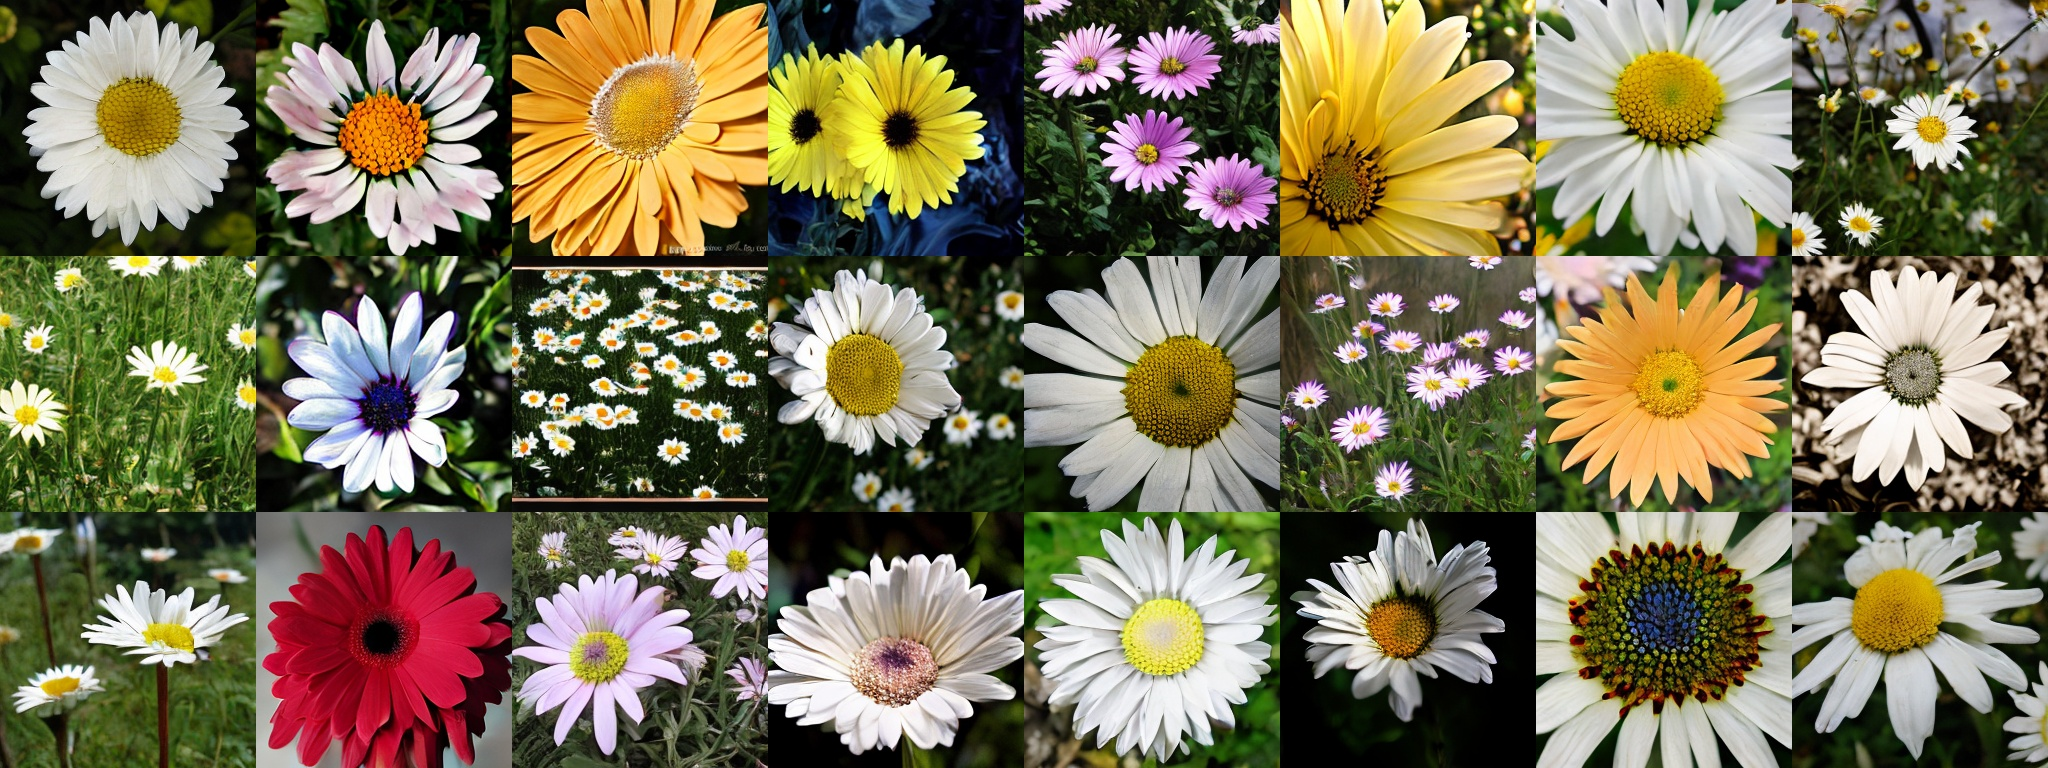
\includegraphics[width=\linewidth]{figures/imf_images/985.jpg}
    \end{minipage}\\[-0.2em]
    \centering\small Class 985: Daisy
    
    \caption{\textbf{Side-by-side comparison with improved MeanFlow (iMF)~\cite{geng2025improved} (page 5/5).} Uncurated samples from our method (left) and iMF (right) on \textbf{all} ImageNet classes visualized in the iMF paper. Both methods generate images with a single neural function evaluation (1-NFE). The iMF visualizations use CFG $\omega{=}6.0$ and interval $[t_\text{min}, t_\text{max}]{=}[0.2, 0.8]$, achieving FID 3.92 and IS 348.2 (DiT-XL/2). For fair comparison, we set the CFG scale to match the IS of iMF visualizations, which leads to FID 3.01 and IS 354.4 (at CFG=1.5) for our method (DiT-L/2).}
    \label{fig:comparison_imf_5}
\end{figure*}
